%============================================================
% MTH 112 Project - Hub File
% Updated 202504
%============================================================

\documentclass[11pt,twoside]{report}
\usepackage{tabularx}
\usepackage{tkz-euclide}
\usepackage{graphicx}
\usepackage{amssymb}
\usepackage{tasks}
\usepackage[standard,framed,thmmarks]{ntheorem}	% needed for theorems, examples
\usepackage{enumerate}
\usepackage{pstricks} % needed for many things, including fancy shading in theorems, examples
\usepackage{enumitem}
\usepackage{placeins} % enables \FloatBarrier, useful for positioning figures/tables more precisely.
\usepackage{calc} % calculations such as dividing textwidth/2
\usepackage{multicol}
\usepackage{framed}	% needed for putting boxes round theorems, examples	
\usepackage{needspace} % needed to keep examples looking good (with \hrule above and below)
\usepackage{fancyhdr} % headers and footersd
%\usepackage{nonfloat} % needed for putting figures in boxes- they don't float!
%\usepackage{refcheck} % useful for checking references
\usepackage{array}
\usepackage{tocloft}
\renewcommand\cftsecafterpnum{\vskip3pt}
\renewcommand\cftchapafterpnum{\vskip5pt}
\setlength{\cftbeforetoctitleskip}{0mm}
\setlength\cftaftertoctitleskip{20pt}
\setlength{\cftbeforechapskip}{4pt}
\usepackage{latexsym}
\usepackage{amscd}
\usepackage{multirow}
\usepackage{amsmath}
\usepackage{textcomp} % for cents symbol
\usepackage{lastpage}
\usepackage{setspace}
\usepackage{caption}
\usepackage{wasysym}
\pagestyle{fancy}
\setlength{\textwidth}{7.25in}			%for =>PDF, use 6.5in
\setlength{\textheight}{9.10in}		%for =>PDF, use 9.5in
\setlength{\oddsidemargin}{-0.375in}
\setlength{\evensidemargin}{-0.375in}
\setlength{\voffset}{-.75in}			%for=>PDF, use -0.75in
\setlength{\footskip}{15pt}
\usepackage[per-mode=symbol]{siunitx}
\usepackage[super]{nth} %nth added when appropriate
\usepackage{qrcode}
\usepackage{dirtytalk} %for quotations
\settasks{after-item-skip=2cm,after-skip=2cm} %for tasks instead of items
\setlength\columnsep{30pt} %space between columns
\newcolumntype{P}[1]{>{\centering\arraybackslash}p{#1}} %center content in cells of table
\usepackage[T1]{fontenc}
\usepackage{lmodern}
\usepackage{url}
\usepackage{mathtools}
\DeclarePairedDelimiter\abs{\lvert}{\rvert}%
\DeclarePairedDelimiter\norm{\lVert}{\rVert}%
\usepackage{harpoon}
% \usepackage{draftwatermark} %Turn on or off for Watermark DRAFT
% \SetWatermarkText{{\color{red!7}{DRAFT}}}
% \SetWatermarkScale{1}

% \ifpdf
  \usepackage{pdfcolmk}
% \fi
% % check if using xelatex rather than pdflatex
% \ifxetex
%   \usepackage{fontspec}
% \fi

\usepackage{pifont} % for dingbats
\providecommand{\HUGE}{\Huge} % if not using memoir
\newlength{\drop} % for my convenience
% specify the Webomints family
\newcommand*{\wb}[2]{\fontsize{#1}{#2}\usefont{U}{webo}{xl}{n}}
% select a (FontSite) font by its font family ID
\newcommand*{\FSfont}[1]{\fontencoding{T1}\fontfamily{#1}\selectfont}
% if you don?t have the FontSite fonts either \renewcommand*{\FSfont}[1]{}
% or use your own choice of family.
% select a (TeX Font) font by its font family ID
\newcommand*{\TXfont}[1]{\fontencoding{T1}\fontfamily{#1}\selectfont}
% Generic publisher?s logo
\newcommand*{\plogo}{\fbox{$\mathcal{PL}$}}
% Some shades
\definecolor{Dark}{gray}{0.2}
\definecolor{MedDark}{gray}{0.4}
\definecolor{Medium}{gray}{0.6}
\definecolor{Light}{gray}{0.8}
% Additional font series macros
\makeatletter
% light series
% e.g., kernel doc, section s: line 12 or thereabouts
\DeclareRobustCommand\ltseries
  {\not@math@alphabet\ltseries\relax
   \fontseries\ltdefault\selectfont}
% e.g., kernel doc, section t: line 32 or thereabouts
\newcommand{\ltdefault}{l}
% e.g., kernel doc, section v: line 19 or thereabouts
\DeclareTextFontCommand{\textlt}{\ltseries}
% heavy(bold) series
\DeclareRobustCommand\hbseries
  {\not@math@alphabet\hbseries\relax
   \fontseries\hbdefault\selectfont}
\newcommand{\hbdefault}{hb}
\DeclareTextFontCommand{\texthb}{\hbseries}
\makeatother

%==================================================
%  TITLE PAGE STUFF
%==================================================
% enumerate settings
\setlist{itemsep=6pt} %topsep=0.1em

%==================================================
%  PGF/TikZ + PGFPlots setup (consolidated)
%==================================================

% TikZ libraries (PGF already loaded earlier via \usepackage{tikz})
\usepackage{tikz}
\usetikzlibrary{
  backgrounds,
  arrows,
  arrows.meta,
  calc,
  calligraphy,
  decorations.fractals,
  decorations.footprints,
  decorations.pathreplacing,
  decorations.text,
  fadings,
  patterns,
  positioning,
  shadows,
  shapes,
  shapes.symbols
}


\tikzset{>=stealth}
\tikzset{tight background}

% PGFPlots
\usepackage{pgfplots}
\pgfplotsset{compat=1.14}
\usepgfplotslibrary{fillbetween}
\usepgfplotslibrary{polar}

\pgfplotsset{
  every axis/.append style={
    draw=black!75,
    width=7cm,
    height=7cm,
    xlabel={$x$},
    ylabel={$y$},
    axis x line=middle,
    axis y line=middle,
    line width=0.75pt,
    tick label style={font=\tiny},
    label style={font=\small},
    legend style={font=\tiny}
  }}

\pgfplotsset{framed/.style={axis background/.style={draw=black!75}}}

\usepackage{hyperref}
% \hypersetup{colorlinks=true,urlcolor=blue,linkcolor=black,breaklinks=true}%for color printing
\hypersetup{colorlinks=true,urlcolor=black,linkcolor=black,breaklinks=true} %for B&W printing
\usepackage{minitoc}
\usepackage{xcolor}
\usepackage[raggedrightboxes]{ragged2e}
%   My colors for screen/color printing
% \definecolor{first}{rgb}{0.08,0.08,0.8}     %blue
% \definecolor{second}{rgb}{0,.55,0.05}       %green
% \definecolor{third}{rgb}{0.54,0.27,0}       %orange
% \definecolor{fourth}{rgb}{0.9,0.1,0.9}      %pink
% \definecolor{fifth}{rgb}{0.6,0.08,.8}       %purple

%   My colors for BW printing
\definecolor{first}{rgb}{0,0,0}
\definecolor{second}{rgb}{0.125,0.125,0.125}
\definecolor{third}{rgb}{0.25,0.25,0.25}
\definecolor{fourth}{rgb}{0.375,0.375,0.375}
\definecolor{fifth}{rgb}{0.5,0.5,0.5}

% \newcommand{\cred}[0]{\color{red}}
% \newcommand{\corange}[0]{\color{orange}}
% \newcommand{\cgreen}[0]{\color{green}}
% \newcommand{\cblue}[0]{\color{blue}}
% \newcommand{\cpurple}[0]{\color{purple}}
% \newcommand{\cbrown}[0]{\color{brown}}
% \newcommand{\cgray}[0]{\color{gray}}

\setlength{\parindent}{0pt}
\date{}

% Prevent bold wasysym warnings in small sizes
\DeclareRobustCommand{\wasybf}{\mdseries}

% Common defaults
\theoremsymbol{}
\theoremseparator{:}
\shadecolor{blue}

% BREAK style: Prep / Exit / Activity / Exercise / Practice
\theoremstyle{break}
\theoremheaderfont{\bfseries}
\theorembodyfont{\normalfont\mdseries\upshape}
\theoremprework{\vspace{1mm}}

\newtheorem{myPrep}{Preparation}
\newtheorem{myExit}{Exit}
\newtheorem{myActivity}{Activity}
\newtheorem{myExercise}{Exercise}
\newtheorem{myPractice}{Practice}

% Definition
\theoremstyle{empty}
\theoremsymbol{}
\newtheorem{myDefinition}{Definition}

% NONUMBERBREAK style: Framed / Properties / Important Note
\theoremstyle{nonumberbreak}
\theoremheaderfont{\bfseries}
\theorembodyfont{\normalfont\mdseries\upshape}

% Framed thing (no separator)
\theoremseparator{}
\newframedtheorem{myFramed}{}

% Properties (tight spacing)
\theoremseparator{:}
\theoremprework{\vspace{-3mm}}
\theorempostwork{\vspace{-4mm}}
\newtheorem{myProperties}{Properties}

% Important Note (keep your tighter prework)
\theoremprework{\vspace{-0.1cm}}
\theorempostwork{}
\newtheorem{myNote}{Important Note}

% Shaded definition box
\def\theoremframecommand{%
  \psshadowbox[fillstyle=solid,fillcolor=yellow!30,linecolor=black]}
\newshadedtheorem{myshadedDefinition}{}

% Utility macros
\newcommand{\ph}{\phantom}
\newcommand{\ds}{\displaystyle}
\newcommand{\resetCounters}{
  \setcounter{myPrep}{0}
  \setcounter{myPractice}{0}
  \setcounter{myActivity}{0}
  \setcounter{myExit}{0}
  \setcounter{myExercise}{0}
}

\newcommand{\fakesubsection}[1]{%
  \par\refstepcounter{subsection} % Increase section counter
  \subsectionmark{#1} % Add section mark (header)
}

\newcommand{\fakesection}[1]{%
  \par\refstepcounter{section} % Increase section counter
  \sectionmark{#1} % Add section mark (header)
  \addcontentsline{toc}{section}{\protect\numberline{\thesection}#1}
}

\newcommand{\fakechapter}[1]{%
  \par\refstepcounter{chapter} % Increase section counter
  \chaptermark{#1} % Add section mark (header)
  \addcontentsline{toc}{chapter}{\protect\numberline{}#1}
}

\newcommand{\exitlikert}[1]{%
On a scale of 1 -- 5, how are you feeling with the concepts related to #1?\\
Place a mark on the scale below to indicate your overall comfort with the topics we saw in this section.
\begin{center}
 
\includegraphics[scale=0.05]{worried} \begin{tabular}{ccccc}
 &  &  &  & \\
\hline
\hspace{1mm}1\hspace{4mm}  & \hspace{4mm}2\hspace{4mm} & \hspace{4mm}3\hspace{4mm} & \hspace{4mm}4\hspace{4mm} & \hspace{4mm}5\hspace{1mm}
\end{tabular} 
\includegraphics[scale=0.05]{grin}
\end{center}
}

\newcommand{\defexample}{{\textit{Example}}:}

\newcommand{\textbook}[1]{ %
\vspace{0.5em}
{\bf Textbook Reference:} This relates to content in \S#1 of {\it Algebra and Trigonometry 2e}.\\[-4mm]}

\newcommand{\textbooks}[2]{ %
\vspace{0.5em}
{\bf Textbook Reference:} This relates to content in \S#1 and \S#2 of {\it Algebra and Trigonometry 2e}.\\[-4mm]}

\makeatletter
\renewcommand{\theHmyPractice}{\thechapter.\thesection.\arabic{myPractice}}
\renewcommand{\theHmyPrep}{\thechapter.\thesection.\arabic{myPrep}}
\renewcommand{\theHmyExit}{\thechapter.\thesection.\arabic{myExit}}
\renewcommand{\theHmyExercise}{\thechapter.\thesection.\arabic{myExercise}}
\renewcommand{\theHmyActivity}{\thechapter.\thesection.\arabic{myActivity}}
\makeatother

\newcommand{\vect}[2]{\left\langle #1,#2 \right\rangle}
\newcommand{\vectr}[1]{\vec{\textbf{#1}}}
\newcommand{\unitv}[1]{\hat{\textbf{#1}}}

\newcommand*{\titleRF}{\begingroup% Robert Frost, T&H p 149
\fontfamily{ptm}\selectfont 
%\setmainfont{Asana-Math} % FontSite Bergamo (Bembo)
\drop = 0.2\textheight
\centering
~
\vfill
\rule{0.7\textwidth}{0.8pt}\\[\baselineskip]
{\HUGE \bf MTH 112 Lab Manual \small v1.3 12/18/2025}\\[0.04\drop]
\rule{0.7\textwidth}{0.8pt}\\[\baselineskip]
%{\Large \plogo}\\[0.5\baselineskip]
%{\large\scshape year}\par
\vfill
\vfill
\vfill
{\large Prepared by \\
Portland Community College\\
Mathematics Department\\ }
\endgroup}

%==================================================

\begin{document}
\pagenumbering{roman}
\setlist[enumerate]{noitemsep,topsep=-10pt,itemsep=-5pt}

\fancyhf{}
\fancyfoot[LE,RO]{\scriptsize{ Page \thepage} }
\fancyfoot[RE,LO]{\scriptsize{ \leftmark }}
\fancyhead[LE,RO]{\scriptsize{ \rightmark }}
\fancyhead[RE,LO]{\scriptsize{ MTH 112 Lab Manual}}
\renewcommand{\headrulewidth}{0.4pt}
\fancyfootoffset[LE,LO]{0in}
\renewcommand{\footrulewidth}{0.4pt}

% ==================================================

\thispagestyle{empty}
\titleRF

\newpage

\dominitoc
\tableofcontents
\singlespacing
\thispagestyle{empty}

\newpage

\cleardoublepage
\pagenumbering{arabic}

\renewcommand{\labelenumi}{\alph{enumi})}
\renewcommand{\labelenumii}{\roman{enumii})}

% Front Matter
 %============================================================
% MTH 112 Project - Front Matter
% Chapter 0 - Front Matter
% Updated 202504
%============================================================

\setcounter{chapter}{-1} 
\chapter{Front Matter}  \label{chapter-frontmatter}

\section*{Colophon}
{\bf Project Lead} Ross Kouzes\\[0.5em]
{\bf Contributing Authors} Shane Horner, Ross Kouzes, Scot Leavitt\\[0.5em]
{\bf Additional Contributors} Amy Cakebread, Bethany Downs, Wendy Fresh, Dave Froemke, Peter Haberman, Shane Horner, Scot Leavitt, Emily Nelson, Kim Neuburger,Emily O’Sullivan,  Jeff Pettit, Dennis Reynolds, Rebecca Ross, Heiko Spoddeck, Greta Swanson, Stephanie Yurasits \\[0.5em]
\copyright 2025 Portland Community College\\[0.5em]
This work is licensed under the Creative Commons Attribution-Noncommercial-ShareAlike (CC BY-NC-SA) 4.0 International License. To view a copy of this license, visit \href{CreativeCommons.org}{https://creativecommons.org/licenses/by-nc-sa/4.0/}\\


\newpage
\vspace{0.75in}

This is the second part of the two part lab manual for MTH 111 and MTH 112 at Portland Community College. The first chapter is \say{Chapter 5} to align with \href{http://tiny.cc/111Z-Supplement}{the first portion of the lab manual}.

\vspace{0.5em}

This lab manual was designed with the intent of being used in the following manner.  In each section:

\setlist{itemsep=6pt}
\begin{itemize}
	\item Students will complete the Preparation Exercises before receiving instruction on the content.  Some instructors will have students do this before coming to class, while others might do it as a warmup in class.
	\item There will be some instructor-led presentation of the content.  This may be a formal class lecture, a discovery activity, a video lecture, or something else.
	\item Students will then engage in Practice Exercises in a group setting to reinforce their initial understanding of the foundational concepts.
	\item An instructor will then assign one or more group activities.  Because many of these activities are web-based and instructors can choose to use different activities, we have not included any of the possible activities in this document. 
	\item The Definitions are meant to provide a single location for all definitions and some key concepts.  Students can use this as a resource after having covered the topics in class.
	\item Students will complete some or all of the Exit Exercises, as decided by their instructor, to summarize their understanding of key concepts.
	\item In general, not every section of this lab manual will take the same amount of class time.  Some sections might be half-day topics, while others could be two-day topics.	
	\item Each instructor will identify for their class which exercises will be submitted as part of the course grade.
\end{itemize}
~

Course Resource Links:\\
{\it Algebra and Trigonometry 2e}:  \href{http://tiny.cc/111Z-Textbook}{http://tiny.cc/112Z-Textbook}\\
MTH 112 Supplement: \href{http://tiny.cc/111Z-Supplement}{http://tiny.cc/112Z-Supplement}

\newpage
~

% Ch7 in book
\setcounter{chapter}{4}
\chapter{The Unit Circle} \label{the-unit-circle}
\minitoc

\begin{center}
    \captionsetup{type=figure} \captionof{figure}{Unit Circle with Standard Values}
    \begin{tikzpicture}
      \begin{axis}[
          xmin=-1,xmax=1,
          ymin=-1,ymax=1,
              xtick={-1,1},
              ytick={-1,1},
              clip=false,
          ]
          \draw   (axis cs:0,0) circle [radius=1];
          \addplot[mark=*,color=first] coordinates{(1,0)} node[right] {\footnotesize$(1,0)$} node[below left] {\footnotesize$\theta=0$};

          \draw   [color=second,opacity=0.2](0,0)--(0.866,0.5);
          \addplot[mark=*,color=second] coordinates{(0.866,0.5)} node[right,rotate=30] {\footnotesize$\left(\frac{\sqrt3}{2},\frac{1}{2}\right)$} node[left,rotate=30] {\footnotesize$\theta=\frac{\pi}{6}$};
          \draw   [color=third,opacity=0.2](0,0)--(0.707,0.707);
          \addplot[mark=*,color=third] coordinates{(0.707,0.707)} node[left,rotate=45] {\footnotesize$\theta=\frac{\pi}{4}$} node[right,rotate=45] {\footnotesize$\left(\frac{\sqrt2}{2},\frac{\sqrt2}{2}\right)$};
          \draw   [color=fourth,opacity=0.2](0,0)--(0.5,0.866);
          \addplot[mark=*,color=fourth] coordinates{(0.5,0.866)} node[left,rotate=60] {\footnotesize$\theta=\frac{\pi}{3}$} node[right,rotate=60] {\footnotesize$\left(\frac{1}{2},\frac{\sqrt3}{2}\right)$};
          
          \draw   [color=fifth](0,0)--(0,1);
          \addplot[mark=*,color=fifth] coordinates{(0,1)} node[below right,rotate=-90] {\footnotesize$\theta=\frac{\pi}{2}$} node[left,rotate=-90] {\footnotesize$(0,1)$};

          \draw   [color=fourth,opacity=0.2](0,0)--(-0.5,0.866);
          \addplot[mark=*,color=fourth] coordinates{(-0.5,0.866)} node[right,rotate=-60] {\footnotesize$\theta=\frac{2\pi}{3}$} node[left,rotate=-60] {\footnotesize$\left(-\frac{1}{2},\frac{\sqrt3}{2}\right)$};
          \draw   [color=third,opacity=0.2](0,0)--(-0.707,0.707);
          \addplot[mark=*,color=third] coordinates{(-0.707,0.707)} node[right,rotate=-45] {\footnotesize$\theta=\frac{3\pi}{4}$} node[left,rotate=-45] {\footnotesize$\left(-\frac{\sqrt2}{2},\frac{\sqrt2}{2}\right)$};
          \draw   [color=second,opacity=0.2](0,0)--(-0.866,0.5);
          \addplot[mark=*,color=second] coordinates{(-0.866,0.5)} node[right,rotate=-30] {\footnotesize$\theta=\frac{5\pi}{6}$} node[left,rotate=-30] {\footnotesize$\left(-\frac{\sqrt3}{2},\frac{1}{2}\right)$};

          \addplot[mark=*,color=first] coordinates{(-1,0)} node[above right] {\footnotesize$\theta=\pi$} node[left] {\footnotesize$(-1,0)$};
          
          \draw   [color=second,opacity=0.2](0,0)--(-0.866,-0.5);
          \addplot[mark=*,color=second] coordinates{(-0.866,-0.5)} node[right,rotate=30] {\footnotesize$\theta=\frac{7\pi}{6}$} node[left,rotate=30] {\footnotesize$\left(-\frac{\sqrt3}{2},-\frac{1}{2}\right)$};
          \draw   [color=third,opacity=0.2](0,0)--(-0.707,-0.707);
          \addplot[mark=*,color=third] coordinates{(-0.707,-0.707)} node[right,rotate=45] {\footnotesize$\theta=\frac{5\pi}{4}$} node[left,rotate=45] {\footnotesize$\left(-\frac{\sqrt2}{2},-\frac{\sqrt2}{2}\right)$};
          \draw   [color=fourth,opacity=0.2](0,0)--(-0.5,-0.866);
          \addplot[mark=*,color=fourth] coordinates{(-0.5,-0.866)} node[right,rotate=60] {\footnotesize$\theta=\frac{4\pi}{3}$} node[left,rotate=60] {\footnotesize$\left(-\frac{1}{2},-\frac{\sqrt3}{2}\right)$};

          \addplot[mark=*,color=fifth] coordinates{(0,-1)} node[above left,rotate=-90] {\footnotesize$\theta=\frac{3\pi}{2}$} node[right,rotate=-90] {\footnotesize$\left(0,-1\right)$};
          
          \draw   [color=second,opacity=0.2](0,0)--(0.866,-0.5);
          \addplot[mark=*,color=second] coordinates{(0.866,-0.5)} node[left,rotate=-30] {\footnotesize$\theta=\frac{11\pi}{6}$} node[right,rotate=-30] {\footnotesize$\left(\frac{\sqrt3}{2},-\frac{1}{2}\right)$};
          \draw   [color=third,opacity=0.2](0,0)--(0.707,-0.707);
          \addplot[mark=*,color=third] coordinates{(0.707,-0.707)} node[left,rotate=-45] {\footnotesize$\theta=\frac{7\pi}{4}$} node[right,rotate=-45] {\footnotesize$\left(\frac{\sqrt2}{2},-\frac{\sqrt2}{2}\right)$};
          \draw   [color=fourth,opacity=0.2](0,0)--(0.5,-0.866);
          \addplot[mark=*,color=fourth] coordinates{(0.5,-0.866)} node[left,rotate=-60] {\footnotesize$\theta=\frac{5\pi}{3}$} node[right,rotate=-60] {\footnotesize$\left(\frac{1}{2},-\frac{\sqrt3}{2}\right)$};
      \end{axis}
    \end{tikzpicture}
  \end{center}

\resetCounters
%============================================================
% MTH 112 Project - Angles
% Updated 202504
%============================================================

\section{Angles} \label{section-angles}
In this section we will draw angles in standard position, convert between degrees and radians and degrees-minutes-seconds, find coterminal angles, and find the length of a circular arc.

\textbook{\href{https://openstax.org/books/algebra-and-trigonometry-2e/pages/7-1-angles}{7.1}}

\subsection*{Preparation Exercises} \label{preparation-exercises-section-angles}

Answer the following without using a calculator. These questions are intended to check the prerequisite skills needed to complete the rest of the lab.

\begin{multicols}{2}
	\begin{myPrep}
		Solve the equation $T=\frac{v}{w^2}$ for $w$.
	\end{myPrep}
	\vfill
	
	\begin{myPrep}
		Simplify the expression $80\cdot\frac{\pi}{180}$ without a calculator. Reduce to simplest form.
	\end{myPrep}
	\vfill
\end{multicols}
\vfill

\begin{myPrep}
In terms of time, how many minutes total are in 3 hours and 53 minutes?
\end{myPrep}
\vfill

\begin{myPrep}
	\begin{minipage}[t]{0.5\linewidth}
		Draw a line segment from the point $(5,-3)$ to the point $(-1,2)$. Find the distance between those two points using the Pythagorean Theorem. Leave your answer in exact form.
		\vfill
	\end{minipage}
	\begin{minipage}[t]{0.5\linewidth}
		\begin{center}\captionsetup{type=figure} \captionof{figure}{A grid to plot your points}
			\begin{tikzpicture}
				\begin{axis}[
					framed,
					xmin=-6,xmax=6,
					ymin=-6,ymax=6,
			       	xtick={-4,-2,2,4},
			       	minor xtick={-5,-3,-1,1,3,5},
			       	ytick={-4,-2,2,4},
			       	minor ytick={-5,-3,-1,1,3,5},
			       	grid=both
					]
				\end{axis}
			\end{tikzpicture}\label{fig:section-angles-myprep1}
		\end{center}
	\end{minipage}
\end{myPrep}
\vfill

%======================================================
\newpage
%======================================================

\subsection*{Practice Exercises} \label{practice-exercises-section-angles}

\begin{myPractice}
	Find an angle that is coterminal to $\ang{-40}$ and is between $\ang{360}$ and $\ang{720}$.
		% Solution: Since $\ang{-40}$ is in Quadrant IV, $\ang{40}$ below the $x$-axis, a coterminal angle would be $\ang{360}-\ang{40}=\ang{320}$. However, this isn't between $\ang{360}$ and $\ang{720}$, so we can add another $\ang{360}$ and we get $\ang{320}+\ang{360}=\ang{680}$. Another way to find this angle is just to subtract $\ang{40}$ from $\ang{720}$: $\ang{720}-\ang{40}=\ang{680}$.
		\vfill
\end{myPractice}

\begin{myPractice}
	Match the pairs of coterminal angles.
			\begin{multicols}{2}
				\begin{itemize}
					\item \ang{30}
					\item \ang{270}
					\item \ang{-220}
					\item \ang{-60}
					\item \ang{0}
					\item \ang{150}
					\columnbreak
					\item \ang{720}
					\item \ang{-90}
					\item \ang{390}
					\item \ang{510}
					\item \ang{-420}
					\item \ang{500}
				\end{itemize}
			\end{multicols}
\end{myPractice}

\begin{myPractice}
	Convert the angles.
			\begin{enumerate}
				\item Convert $\ang{28}$ to radians. Leave your answer as a fraction in terms of $\pi$.
				\vfill
				\item Convert $\frac{7\pi}{9}$ radians to degrees. Round to 6 digits behind the decimal place.
				\vfill

%======================================================
\newpage
%======================================================

				\item Convert $\ang{14;20;36}$ to a decimal measurement of degrees. 
				\vfill
				\item Convert $\ang{76.85}$ to degrees-minutes-seconds.
				\vfill
			\end{enumerate}
\end{myPractice}

\begin{myPractice}
	Use the formula $s=r\theta$ to find the missing values.
			\begin{enumerate}
				\item Find the arc length of on a circle of radius $6$ with an interior angle of $\frac{4\pi}{7}$.
				\vfill
				\item Find the interior angle of an arc length on a circle of radius $12$ with an arc length of $\frac{3\pi}{2}$.
				\vfill
				\item Find the arc length of on a circle of radius $10\pi$ with an interior angle of $\ang{20}$.
				\vfill
			\end{enumerate}
		\vfill
\end{myPractice}

%======================================================
\newpage
%======================================================

\subsection*{Definitions} \label{definitions-section-angles}
\begin{multicols}{2}
	\begin{myDefinition}[{Angle}]~\\[0.5mm]
		An \textbf{angle} is formed when two lines intersect at a point. We can measure the \say{size} of this angle in degrees or radians.
	\end{myDefinition}
	\begin{myDefinition}[{Ray}]~\\[0.5mm]
		A \textbf{ray} is a portion of a line that starts at a point and extends infinitely in one direction.
	\end{myDefinition}
	\begin{myDefinition}[{Degree}]~\\[0.5mm]
		A \textbf{degree} is an angle measurement equal to $\frac{1}{360}$ of a full rotation.
	\end{myDefinition}
	\begin{myDefinition}[{Right Angle}]~\\[0.5mm]
		 A \textbf{right angle} is an angle of $\ang{90}$.
	\end{myDefinition}
	\begin{myDefinition}[{Radian}]~\\[0.5mm]
			A \textbf{radian} is a unit of measurement of angle size, and 1 radian is defined to be the angle that is made when the arc length for that angle on a circle of radius 1 is equal to 1. \href{http://tiny.cc/radian-definition}{Check out this Desmos link} and click the "play" button on the slider for a visual representation of this concept. \qrcode[height=1cm]{http://tiny.cc/radian-definition}
	\end{myDefinition}

	\begin{center}
		\captionsetup{type=figure} \captionof{figure}{Standard Angles}
		\begin{tikzpicture}
			\begin{axis}[
					xmin=-1,xmax=1,
					ymin=-1,ymax=1,
		       		xtick={-1,1},
		       		ytick={-1,1},
		       		clip=false,
					]
					\draw 	(axis cs:0,0) circle [radius=1];
					\addplot[mark=*,color=first] coordinates{(1,0)} node[below left] {\footnotesize$\theta=0$};

					\draw   [color=second,opacity=0.2](0,0)--(0.866,0.5);
					\addplot[mark=*,color=second] coordinates{(0.866,0.5)} node[left,rotate=30] {\footnotesize$\theta=\frac{\pi}{6}$};
					\draw   [color=third,opacity=0.2](0,0)--(0.707,0.707);
					\addplot[mark=*,color=third] coordinates{(0.707,0.707)} node[left,rotate=45] {\footnotesize$\theta=\frac{\pi}{4}$};

					\draw   [color=fourth,opacity=0.2](0,0)--(0.5,0.866);
					\addplot[mark=*,color=fourth] coordinates{(0.5,0.866)} node[left,rotate=60] {\footnotesize$\theta=\frac{\pi}{3}$};

					\addplot[mark=*,color=fifth] coordinates{(0,1)}node[below right,rotate=-90] {\footnotesize$\theta=\frac{\pi}{2}$};

					\draw   [color=fourth,opacity=0.2](0,0)--(-0.5,0.866);
					\addplot[mark=*,color=fourth] coordinates{(-0.5,0.866)}node[right,rotate=-60] {\footnotesize$\theta=\frac{2\pi}{3}$};

					\draw   [color=third,opacity=0.2](0,0)--(-0.707,0.707);
					\addplot[mark=*,color=third] coordinates{(-0.707,0.707)}node[right,rotate=-45] {\footnotesize$\theta=\frac{3\pi}{4}$};

					\draw   [color=second,opacity=0.2](0,0)--(-0.866,0.5);
					\addplot[mark=*,color=second] coordinates{(-0.866,0.5)}node[right,rotate=-30] {\footnotesize$\theta=\frac{5\pi}{6}$};

					\addplot[mark=*,color=first] coordinates{(-1,0)} node[above right] {\footnotesize$\theta=\pi$};
					\draw   [color=second,opacity=0.2](0,0)--(-0.866,-0.5);
					\addplot[mark=*,color=second] coordinates{(-0.866,-0.5)} node[right,rotate=30] {\footnotesize$\theta=\frac{7\pi}{6}$};
					\draw   [color=third,opacity=0.2](0,0)--(-0.707,-0.707);
					\addplot[mark=*,color=third] coordinates{(-0.707,-0.707)} node[right,rotate=45] {\footnotesize$\theta=\frac{5\pi}{4}$};
					\draw   [color=fourth,opacity=0.2](0,0)--(-0.5,-0.866);
					\addplot[mark=*,color=fourth] coordinates{(-0.5,-0.866)} node[right,rotate=60] {\footnotesize$\theta=\frac{4\pi}{3}$};

					\addplot[mark=*,color=fifth] coordinates{(0,-1)} node[above left,rotate=-90] {\footnotesize$\theta=\frac{3\pi}{2}$};
					\draw   [color=second,opacity=0.2](0,0)--(0.866,-0.5);
					\addplot[mark=*,color=second] coordinates{(0.866,-0.5)} node[left,rotate=-30] {\footnotesize$\theta=\frac{11\pi}{6}$};
					\draw   [color=third,opacity=0.2](0,0)--(0.707,-0.707);
					\addplot[mark=*,color=third] coordinates{(0.707,-0.707)} node[left,rotate=-45] {\footnotesize$\theta=\frac{7\pi}{4}$};
					\draw   [color=fourth,opacity=0.2](0,0)--(0.5,-0.866);
					\addplot[mark=*,color=fourth] coordinates{(0.5,-0.866)} node[left,rotate=-60] {\footnotesize$\theta=\frac{5\pi}{3}$};
			\end{axis}
		\end{tikzpicture}
		\label{fig:Unit-circle-values-angles}
	\end{center}
% \end{multicols}

% \begin{multicols}{2}
	\begin{myDefinition}[{Initial and Terminal sides}]~\\[0.5mm]
		An angle is created by imagining two rays originating from the same point: the \textbf{initial side} of the angle is stationary and the \textbf{terminal side} is rotated around until the desired angle is created. Angles measured from initial to terminal side in a counter-clockwise direction are positive. Angles measured from initial to terminal side clockwise are negative.
	\end{myDefinition}
	\begin{myDefinition}[{Standard Position}]~\\[0.5mm]
		An angle is said to be in \textbf{standard position} if the initial and terminal sides of the angle meet at the origin and the initial side of the angle is along the positive $x$-axis.
	\end{myDefinition}
	\begin{myDefinition}[{Coterminal}]~\\[0.5mm]
		Two angles are \textbf{coterminal} if their initial and terminal sides align, but they differ by an integer number of full rotations. In standard position, this means that the two angles are \say{in the same place} are different by some integer multiple of $\ang{360}$ (or $2\pi$ radians).
	\end{myDefinition}
	\begin{myDefinition}[{Arc length}]~\\[0.5mm]
		An \textbf{arc length} is a distance along a part of the circumference of a circle. A formula for arc length is $s=r\theta$, where $s$ stands for arc length along a circle of radius $r$, with an interior angle $\theta$ centered at the center of the circle.
	\end{myDefinition}
	
	\begin{center}
		\captionsetup{type=figure} \captionof{figure}{Coterminal angles $\theta$ and $\alpha$}
		\begin{tikzpicture}
			\begin{axis}[
				% framed,
				xmin=-10,xmax=10,
				ymin=-10,ymax=10,
		       	xtick=\empty,
		       	% minor xtick={-5,5},
		       	ytick=\empty,
		       	% minor ytick={-5,5},
		       	% grid=both,
		       	clip=false
				]
				\draw 	(axis cs:0,0) circle [radius=10];
				
				\draw   [color=first, very thick](10,0)--(5,0)coordinate[label=below:\tiny{initial side}]--(0,0)--(-6,8) coordinate[label=above left:{$\theta$ and $\alpha$ are coterminal}];

				\draw 	(-3,4) node[below,color=third,rotate=-atan(4/3)] {\tiny{terminal side}};
				
				\addplot[variable=\t, domain=0:(atan(-4/3)+180), samples=50, color=first, very thick,-{latex}]({2*cos(t)}, {2*sin(t)});
				
				\draw 	(2,1) node[right,color=first] {$\theta$};
				
				% \addplot[variable=\t, domain=0:(atan(-4/3)+180), samples=50, color=second,very thick]({10*cos(t)}, {10*sin(t)});
				
				\draw[postaction={decorate},very thick,color=second,decoration={text along path,raise=5pt,text color=second,text={arc length for angle {$\theta$}},text align=center}] (-6,8) arc [start angle=atan(-4/3)+180,end angle=0,radius=10];
				
				\addplot[variable=\t, domain=(atan(-4/3)+180):360, samples=50, color=fourth,{latex}-]({2*cos(t)}, {2*sin(t)});
				
				\draw 	(-2,-1) node[left,color=fourth] {$\alpha$};
				\end{axis}
		\end{tikzpicture}
		\label{fig:angle-defs}
	\end{center}
\end{multicols}

%======================================================
\newpage
%======================================================

\subsection*{Exit Exercises} \label{exit-exercises-section-angles}

\begin{myExit} 
Explain why $\ang{-90}$ is not {\it the same} as $\ang{270}$.
\end{myExit}
\vfill

\begin{myExit} 
Convert $\ang{34;29;24}$ to decimal degrees.
\end{myExit}
\vfill
\vfill

\begin{myExit} 
	Convert the angle $\ang{144}$ to radians. Write you answer in exact form as a fraction with $\pi$ in it.
\end{myExit}
\vfill

\begin{myExit} 
	\begin{minipage}[t]{0.6\linewidth}
		How big of an arc length will an angle of $\frac{3\pi}{8}$ radians create on a circle of radius 6? Draw this angle and arc length on the circle of radius 6 provided.
	\end{minipage}
	\begin{minipage}[t]{0.4\linewidth}
		\begin{center}
			\captionsetup{type=figure} \captionof{figure}{A circle of radius 6}
			\begin{tikzpicture}
				\begin{axis}[
					framed,
					xmin=-8,xmax=8,
					ymin=-8,ymax=8,
	        		xtick={-6,-4,-2,2,4,6},
	        		ytick={-6,-4,-2,2,4,6},
	        		grid=both
					]
					\draw[thick,color=first] (0,0) circle (6);
				\end{axis}
			\end{tikzpicture}
		\end{center}
		\label{fig:section-angles-myexit-circle}
	\end{minipage}
\end{myExit}
\vfill
\exitlikert{angles}
\resetCounters
\newpage
~
%============================================================
% MTH 112 Project - Right Triangle Trigonometry
% Updated 202504
%============================================================
% Issue: Include nepal flag
% 2015 Constitution
% The Constitutional Assembly of Nepal adopted 16 November the Constitution of the Federal Democratic Republic of Nepal. In article 8 and Schedule 1 the flag was described.

% Constitution of the Federal Democratic Republic of Nepal
% 8. National flag
% (1) The national flag of Nepal, consists of two juxtaposed triangular figures with a crimson colored base and deep blue borders, there being a white emblem of the crescent moon with eight rays visible out of sixteen in the upper part and a white emblem of a twelve rayed sun in the lower part.
% (2) The method of drawing the flag and other particulars relating thereto shall be as set out in Schedule 1.

% Schedule 1 (Related with clause (2) of Article 8)
% Method of Making the National Flag of Nepal
% (A) Method of Making the shape inside the Border
% (1) On the lower portion of a crimson cloth draw a line AB of the required length from left to right.
% (2) From A draw a line AC perpendicular to AB making AC equal to AB plus one third AB. From AC mark off D making the line AD equal to line AB. Join BD.
% (3) From BD mark off E making BE equal to AB.
% (4) Touching E draw a line FG, starting from the point F on line AC, parallel to AB to the right hand-side. Mark off FG equal to AB.
% (5) Join CG.

% (B) Method of making the Moon
% (6) From AB mark off AH making AH equal to one-fourth of line AB and starting from H draw a line HI parallel to line AC touching line CG at point I.
% (7) Bisect CF at J and draw a line JK parallel to AB touching CG at point K.
% (8) Let L be the point where lines JK and HI cut one another.
% (9) Join JG.
% (10) Let M be the point where line JG and HI cut one another.
% (11) With center M and with a distance shortest from M to BD mark off N on the lower portion of line HI.
% (12) Touching M and starting from O, a point on AC, draw a line from left to right parallel to AB.
% (13) With center L and radius LN draw a semi-circle on the lower portion and let P and Q be the points where it touches the line OM respectively.
% (14) With the center M and radius MQ draw a semi-circle on the lower portion touching P and Q.
% (15) With center N and radius NM draw an arc touching PNQ at R and S. Join RS. Let T be the point where RS and HI cut one another.
% (16) With center T and radius TS draw a semi-circle on the upper portion of PNQ touching at two points.
% (17) With center T and radius TM draw an arc on the upper portion of PNQ touching at two points.
% (18) Eight equal and similar triangles of the moon are to be made in the space lying inside the semi-circle of No (16) and outside the arc of No (17) of his Schedule.

% (C) Method of Making the Sun
% (19) Bisect line AF at U, and draw a line UV parallel to AB line touching line BE at V.
% (20) With center W, the point where HI and UN cut one another and radius MN draw a circle.
% (21) With center W and radius LN draw a circle.
% (22) Twelve equal and similar triangles of the sun are to be made in the space enclosed by the circle of No (20) and No (21) with the two apexes of two triangles touching line HI.

% (D) Method of Making the Border
% (23) The width of the border will be equal to the width of TN. This will be of deep blue color and will be provided on all the sides of the flag. However, on the given angles of the flag the external angles will be equal to the internal angles.
% (24) The above mentioned border will be provided if the flag is to be used with a rope. On the other hand, if it is to be hoisted on a pole, the hole on the border on the side AC can be extended according to requirements.
% Explanation:- The lines HI, RS, FE, ED, JG, OQ, JK and UV are imaginary. Similarly, the external and internal circles of the sun and the other arcs except the crescent moon are imaginary. These are not shown on the flag.



\section{Right Triangle Trigonometry} \label{section-right-triangle-trigonometry}
In this section we will use right triangles to evaluate trigonometric functions, find function values for $\ang{30}$, $\ang{45}$, and $\ang{60}$, use all six trigonometric functions to find lengths inside right triangles, and use right-triangle trigonometry to solve applied problems.

\textbook{\href{https://openstax.org/books/algebra-and-trigonometry-2e/pages/7-2-right-triangle-trigonometry}{7.2}}

\subsection*{Preparation Exercises} \label{preparation-exercises-section-right-triangle-trigonometry}

Answer the following without using a calculator. These questions are intended to check the prerequisite skills needed to complete the rest of the lab.

\begin{myPrep}
	What does the word \say{adjacent} mean?
	\vfill
\end{myPrep}

\begin{myPrep}
	Fill in the table with the missing angle measurements.
			\begin{center}
			\renewcommand{\arraystretch}{1.5} 
				\begin{tabular}{|| c | P{1cm} | P{1cm} | P{1cm} | P{1cm} | P{1cm} | P{1cm} | P{1cm} | P{1cm} ||}
					\hline
					Angle (radians) & $\frac{\pi}{4}$ &  &  & $\frac{2\pi}{3}$ & $\frac{5\pi}{6}$ &  & $\pi$ &  \\
					\hline
					Angle (degrees) &  & $\ang{30}$ & $\ang{90}$ &  &  & $\ang{60}$ &  & $\ang{135}$ \\ 
					\hline
				\end{tabular}
			\end{center}
			\vfill
\end{myPrep}

\begin{myPrep}
	\parbox[t]{0.6\linewidth}{
					Recall that \say{similar triangles} are two triangles with equal angle measurements, but not necessarily equal side lengths. The ratio of any two corresponding sides of the triangles will be equal, which means that $\frac{A_1}{b_1}=\frac{A_2}{b_2}=\frac{A_3}{b_3}$.
					}
						\raisebox{-\height}{
						\begin{tikzpicture}[scale=0.3]
							\draw   (0,0)--(1.5,0) coordinate[label=below:$b_1$]--
        							(3,0)--(3,2) coordinate[label=right:$b_2$]--
        							(3,4)--(1.5,2) coordinate[label=above left:$b_3$]--cycle;
        					
        					\draw   (5,0)--(8,0) coordinate[label=below:$A_1$]--
        							(11,0)--(11,4) coordinate[label=right:$A_2$]--
        							(11,8)--(8,4) coordinate[label=above left:$A_3$]--cycle;
        					
        					\draw   (2.5,0)--(2.5,.5)--(3,.5)--(3,0)--cycle;
        					\draw  	(11,0)--(11,.5)--(10.5,.5)--(10.5,0)--cycle;
						\end{tikzpicture}
						}

				\parbox[t]{0.6\linewidth}{
					Using the similar triangles equations, solve for the missing sides. Drawing may not be drawn to scale.
					}
						\raisebox{-\height}{
						\begin{tikzpicture}[scale=0.4]
							\draw   (0,0)--(1.5,0) coordinate[label=below:$6$]--
        							(3,0)--(3,2) coordinate[label=right:$y$]--
        							(3,4)--(1.5,2) coordinate[label=above left:$8$]--cycle;
        					\draw   (4,0)--(7,0) coordinate[label=below:$9$]--
        							(10,0)--(10,4) coordinate[label=right:$Y$]--
        							(10,8)--(7,4) coordinate[label=above left:$Z$]--cycle;
        					\draw   (2.5,0)--(2.5,.5)--(3,.5)--(3,0)--cycle;
        					\draw  	(10,0)--(10,.5)--(9.5,.5)--(9.5,0)--cycle;
						\end{tikzpicture}
						}
\end{myPrep}
\vfill

%======================================================
\newpage
%======================================================

\subsection*{Practice Exercises} \label{practice-exercises-section-right-triangle-trigonometry}

\begin{myPractice}
	Decide which values match without a calculator using \say{SOHCAHTOA} and \say{CHOSHACAO}. The triangles are not shown to scale.
		\begin{enumerate}
			\begin{multicols}{2}
				\item Which of the values will be the same as $\sin(\ang{40})$?
					\begin{itemize}
						\item $\sin(\ang{50})$
						\item $\cos(\ang{50})$
						\item $\tan(\ang{40})$
						\item $\cos(\ang{40})$
					\end{itemize}
				\columnbreak
					\begin{center}\captionsetup{type=figure} \captionof{figure}{A right triangle}
						\begin{tikzpicture}[thin] \label{section-right-triangle-trig-example-triangle}
							\coordinate (O) at (0,0);
							\coordinate (A) at (2,0);
							\coordinate (B) at (0,3);
							\draw (O)--(A)--(B)--cycle;
							\footnotesize
							\tkzLabelSegment[below=2pt](O,A){$a$}
							\tkzLabelSegment[left=2pt](O,B){$b$}
							\tkzLabelSegment[above=2pt, rotate=-atan(3/2)](A,B){$c$}
							\tkzMarkRightAngle[size=0.5](A,O,B)
							\tkzMarkAngle[size=0.9cm](B,A,O)
							\tkzLabelAngle[pos = 0.6](B,A,O){$\ang{50}$}
							\tkzMarkAngle[size=0.7cm](O,B,A)
							% \tkzLabelAngle[pos = 0.5](O,B,A){$\beta$}
						\end{tikzpicture}
					\end{center}
				\end{multicols}

			\begin{multicols}{2}
				\item Which of the values will be the same as $\tan(\ang{20})$?
					\begin{itemize}
						\item $\cot(\ang{20})$
						\item $\tan(\ang{70})$
						\item $\cot(\ang{70})$
						\item $\cos(\ang{70})$
					\end{itemize}
				\columnbreak
					\begin{center}\captionsetup{type=figure} \captionof{figure}{A right triangle}
						\begin{tikzpicture}[thin] \label{section-right-triangle-trig-example-triangle2}
							\coordinate (O) at (0,0);
							\coordinate (A) at (5,0);
							\coordinate (B) at (0,2);
							\draw (O)--(A)--(B)--cycle;
							\footnotesize
							\tkzLabelSegment[below=2pt](O,A){$x$}
							\tkzLabelSegment[left=2pt](O,B){$y$}
							\tkzLabelSegment[above=2pt, rotate=-atan(2/5)](A,B){$z$}
							\tkzMarkRightAngle[size=0.5](A,O,B)
							\tkzMarkAngle[size=1.3cm](B,A,O)
							\tkzLabelAngle[pos = 1](B,A,O){$\ang{20}$}
							\tkzMarkAngle[size=0.7cm](O,B,A)
							% \tkzLabelAngle[pos = 0.5](O,B,A){$\beta$}
						\end{tikzpicture}
					\end{center}
				\end{multicols}
		\end{enumerate}
\end{myPractice}

\begin{myPractice}
	\begin{multicols}{2}
		For the triangle shown in Figure \ref{section-right-triangle-trig-example-triangle-solving2}, find $a$, $c$, and $\alpha$. You can use a calculator to help get an approximation, accurate to 4 digits behind the decimal place.
		\columnbreak
		\begin{center}\captionsetup{type=figure}\captionof{figure}{A right triangle}
			\begin{tikzpicture}[thin] \label{section-right-triangle-trig-example-triangle-solving2}
				\coordinate (O) at (0,0);
				\coordinate (A) at (7,0);
				\coordinate (B) at (0,3);
				\draw (O)--(A)--(B)--cycle;
				\footnotesize
				\tkzLabelSegment[below=2pt](O,A){$a$}
				\tkzLabelSegment[left=2pt](O,B){$28\text{m}$}
				\tkzLabelSegment[above right=2pt](A,B){$c$}
				\tkzMarkRightAngle[size=0.5](A,O,B)
				\tkzMarkAngle[size=0.8cm](B,A,O)
				\tkzLabelAngle[pos = 0.6](B,A,O){$\alpha$}
				\tkzMarkAngle[size=0.7cm](O,B,A)
				\tkzLabelAngle[pos = 0.5](O,B,A){$\ang{58}$}
			\end{tikzpicture}
		\end{center}
	\end{multicols}
\end{myPractice}
\vfill
\vfill

%======================================================
\newpage
%======================================================

\begin{myPractice}
	On a backpacking trip in the Wallowa Mountains of northeastern Oregon, Megan and Emily were marveling at the height of an enormous Ponderosa Pine. Ross said, \say{we can calculate it's height pretty easily just by knowing that \say{a pace} is $3\text{ft}$ and the distance from the tip of my thumb to the tip of my pinkie is $9$ inches}. Ross paced away from the tree on level ground $30$ paces. Help the three hikers measure the height of the tree two different ways.
	\begin{enumerate}
		\begin{multicols}{2}
			\item Ross finds a stick and measures it to be about $6\text{ft}$ tall. He lays down on the ground and asks Emily to hold the stick vertically on the ground at a certain point where the tip of the stick lines up with the tip of the tree from his point of view. That distance on the ground was $4\text{ft}$ from Ross's viewing position, as shown in Figure \ref{figure-right-triangle-trig-practice-tree-1}. Set up similar triangles to estimate the height of the tree. Drawing not to scale.
			\begin{center}
				\begin{tikzpicture}
					\begin{axis}[
						axis x line=none,
						axis y line=none,
						xlabel=none,
						ylabel=none,
						xmin=-5,xmax=110,
						ymin=-5,ymax=140,
						clip=false,
						]	
							\node   [inner sep=0pt] (Ponderosa) at (88,67) {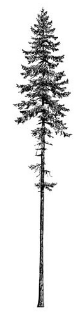
\includegraphics[width=.069\textwidth]{Ponderosalookalike.png}};
							\draw   [color=second,thin](0,0)--(90,0)--(90,135)--cycle;
							\draw   [color=second,thin](83,0)--(83,8)--(90,8);
							\draw   [thin,color=third](0,-10)--(0,-15)--(90,-15)--(90,-10);
							\draw   [color=third](45,-15) coordinate[label=below:$90$ft];

							\draw   [thin,color=first](5.4,0)--(5.4,3)--(8,3);
							\draw   [thin,color=fourth](0,-1)--(0,-2)--(8,-2)--(8,-1);
							\draw   [color=fourth](4,-1) coordinate[label=below:\tiny{$4$ft}];

        					\draw   [very thick,color=first](8,0)--(8,12);
        					\draw   [thin,color=first](10,1)--(11,1)--(11,12)--(10,12);
							\draw   [color=first](10,7) coordinate[label=right:\footnotesize{$6$ft stick}];
					\end{axis}
				\end{tikzpicture}
			\end{center}\captionsetup{type=figure}\captionof{figure}{A tree in the woods}\label{figure-right-triangle-trig-practice-tree-1}
		\end{multicols}
		\vfill

		\begin{multicols}{2}
			\item Ross then took out his phone and used the inclinometer app on to measure the angle to to top of the tree, to be about $\ang{55}$. In this scenario, Ross still $30$ paces away from the tree, and was standing to measure the height: the phone was $5\text{ft}$ above the ground, as shown in Figure \ref{figure-right-triangle-trig-practice-tree-2}. Use right-triangle trigonometry to estimate the height of the tree. Drawing not to scale.
			\begin{center}
				\begin{tikzpicture}
					\begin{axis}[
						axis x line=none,
						axis y line=none,
						xlabel=none,
						ylabel=none,
						xmin=-5,xmax=110,
						ymin=-5,ymax=140,
						clip=false,
						]
							\node   [inner sep=0pt] (Ponderosa) at (88,67) {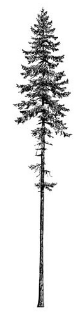
\includegraphics[width=.069\textwidth]{Ponderosalookalike.png}};
							\draw   [thin,color=second](0,0)--(90,0)--(90,135)--(0,10)--cycle;
							\draw   [color=second,thin](83,0)--(83,8)--(90,8);
							\draw   [color=first](-1,5) coordinate[label=left:\footnotesize{$5$ft}];
        					\draw   [thin,color=first](-2,0)--(-3,0)--(-3,10)--(-2,10);
							\draw   [color=third](45,-10) coordinate[label=below:$90$ft];
							\draw   [thin,color=third](0,-5)--(0,-10)--(90,-10)--(90,-5);
							\draw   [color=fourth](10,16)coordinate[label=right:\footnotesize$\ang{55}$];
							\draw   [thin,dashed,color=fourth] (90,10)--(0,10);
        					\addplot[variable=\t, domain=0:55, samples=50,very thin, color=fourth]({8*cos(t)}, {8*sin(t)+10});  
					\end{axis}
				\end{tikzpicture}
			\end{center}\captionsetup{type=figure}\captionof{figure}{A tree in the woods}\label{figure-right-triangle-trig-practice-tree-2}
		\end{multicols}
		\vfill
	\end{enumerate}
\end{myPractice}

%======================================================
\newpage
%======================================================

\subsection*{Definitions} \label{definitions-section-right-triangle-trig}

Consider the triangle shown in Figure \ref{section-right-triangle-trig-definitions}.
		\begin{center}
			\begin{tikzpicture}[thin]
				\coordinate (O) at (0,0);
				\coordinate (A) at (5,0);
				\coordinate (B) at (5,3);
				\draw (O)--(A)--(B)--cycle;
				\footnotesize
				\tkzLabelSegment[below=2pt](O,A){Adjacent}
				\tkzLabelSegment[above=2pt,rotate=atan(3/5)](O,B){Hypotenuse}
				\tkzLabelSegment[above=2pt,rotate=-90](A,B){Opposite}

				\tkzMarkRightAngle[size=0.5](O,A,B)
				% \tkzMarkAngle[size=0.8cm](O,B,A)
				% \tkzLabelAngle[pos = 0.6](O,B,A)
				\tkzMarkAngle[size=0.9cm](A,O,B)
				\tkzLabelAngle[pos = 0.7](A,O,B){$\theta$}
			\end{tikzpicture}\captionsetup{type=figure}\captionof{figure}{A right triangle}\label{section-right-triangle-trig-definitions}
		\end{center}

\begin{myDefinition}[{SOHCAHTOA}]~\\[0.5mm]
	\say{SOHCAHTOA} stands for 
	\begin{itemize}
		\item \textbf{S}ine is \textbf{O}pposite over \textbf{H}ypotenuse
		\item \textbf{C}osine is \textbf{A}djacent over \textbf{H}ypotenuse
		\item \textbf{T}angent is \textbf{O}pposite over \textbf{A}djacent
	\end{itemize}

	These mean the following:

	\begin{itemize}
		\begin{multicols}{3}
			\item  $\sin(\theta)=\frac{\text{Opposite}}{\text{Hypotenuse}}$
			\item  $\cos(\theta)=\frac{\text{Adjacent}}{\text{Hypotenuse}}$
			\item  $\tan(\theta)=\frac{\text{Opposite}}{\text{Adjacent}}$
		\end{multicols}
	\end{itemize}
\end{myDefinition}

\vfill
\begin{myDefinition}[{CHOSHACAO}]~\\[0.5mm]
	\label{CHOSHACAO}
	\say{CHOSHACAO} stands for 
	\begin{itemize}
		\item \textbf{C}osecant is \textbf{H}ypotenuse over \textbf{O}pposite
		\item \textbf{S}ecant is \textbf{H}ypotenuse over \textbf{A}djacent
		\item \textbf{C}otangent is \textbf{A}djacent over \textbf{O}pposite
	\end{itemize}

	These mean the following:

	\begin{itemize}
		\begin{multicols}{3}
			\item  $\csc(\theta)=\frac{\text{Hypotenuse}}{\text{Opposite}}$
			\item  $\sec(\theta)=\frac{\text{Hypotenuse}}{\text{Adjacent}}$
			\item  $\cot(\theta)=\frac{\text{Adjacent}}{\text{Opposite}}$
		\end{multicols}
	\end{itemize}
\end{myDefinition}
\vfill
%======================================================
\newpage
%======================================================

\subsection*{Exit Exercises} \label{exit-exercises-section-right-triangle-trigonometry}

\begin{myExit}
Use the triangle in Figure \ref{figure-right-triangle-trig-exit-triangle} to answer the questions below.
	\begin{center}
		\begin{tikzpicture}[thin]
		%36, 77, 85
			\coordinate (O) at (0,0);
			\coordinate (A) at (3,0);
			\coordinate (B) at (0,2);
			\draw (O)--(A)--(B)--cycle;
			\footnotesize
			\tkzLabelSegment[below=2pt](O,A){$77\text{cm}$}
			\tkzLabelSegment[above=2pt,rotate=90](O,B){$36\text{cm}$}
			\tkzLabelSegment[above=2pt,rotate=-atan(2/3)](A,B){$85\text{cm}$}
			\tkzMarkRightAngle[size=0.5](A,O,B)
			\tkzMarkAngle[size=0.8cm](B,A,O)
			\tkzLabelAngle[pos = 0.6](B,A,O){$\phi$}
			\tkzMarkAngle[size=0.7cm](O,B,A)
			\tkzLabelAngle[pos = 0.5](O,B,A){$\theta$}
		\end{tikzpicture}
	\end{center}\captionsetup{type=figure} \captionof{figure}{A right triangle}\label{figure-right-triangle-trig-exit-triangle}
	\begin{enumerate}[label=(\roman*)]
		\begin{multicols}{3}
			\item Find the value of $\cos(\theta)$.
			\item Find the value of $\tan(\phi)$.
			\item Find the value of $\csc(\theta)$.
		\end{multicols}
	\end{enumerate}
\end{myExit}
\vfill

\begin{myExit}
	Shown in Figure \ref{figure-right-triangle-trig-exit-triangle-SOHCAHTOA} is a triangle with side $b=11$, angle $B=\ang{22}$, and angle $C=\ang{90}$. Find the length of the side $a$.
		\begin{center}
			\begin{tikzpicture}[thin] 
				\coordinate (O) at (0,0);
				\coordinate (A) at (5,0);
				\coordinate (B) at (0,3);
				\draw (O)--(A)--(B)--cycle;
				\footnotesize
				\tkzLabelSegment[below=2pt](O,A){$a$}
				\tkzLabelSegment[left=2pt](O,B){$11$}
				\tkzLabelSegment[above right=2pt](A,B){$c$}
				\tkzMarkRightAngle[size=0.5](A,O,B)
				\tkzMarkAngle[size=1.2cm](B,A,O)
				\tkzLabelAngle[pos = 0.6, left](B,A,O){\footnotesize$\ang{22}$}
				\tkzMarkAngle[size=0.7cm](O,B,A)
				\tkzLabelAngle[pos = 0.5](O,B,A){$A$}
			\end{tikzpicture}
		\end{center}\captionsetup{type=figure}\captionof{figure}{A right triangle}\label{figure-right-triangle-trig-exit-triangle-SOHCAHTOA}
\end{myExit}
\vfill
\exitlikert{right triangle trigonometry}
\resetCounters
\newpage
~
%============================================================
% MTH 112 Project - Unit Circle
% Updated 202504
%============================================================

\section{The Unit Circle} \label{section-unit-circle}
In this section we will find function values for the sine and cosine of $\ang{30}$, $\ang{45}$, and $\ang{60}$, identify the domain and range of sine and cosine functions, find reference angles, and use reference angles to evaluate trigonometric functions.

\textbook{\href{https://openstax.org/books/algebra-and-trigonometry-2e/pages/7-3-unit-circle}{7.3}}

\subsection*{Preparation Exercises} \label{preparation-exercises-section-unit-circle}
Answer the following without using a calculator. These questions are intended to check the prerequisite skills needed to complete the rest of the lab.
%28, 45, 53

\begin{myPrep}
	For a right triangle with side $a=\frac{1}{2}$ and hypotenuse $c=1$, find the missing side, $b$, using the Pythagorean Theorem.
\end{myPrep}
\vfill

\begin{myPrep}
	Which quadrant are the following angles in?
		\begin{enumerate}[label=(\roman*)]
			\begin{multicols}{4}
				\item $\frac{3\pi}{4}$
				\vspace{1cm}
				\item $\frac{4\pi}{3}$
				\item $\frac{11\pi}{6}$
				\vspace{1cm}
				\item $\frac{\pi}{3}$
				\item $-\frac{\pi}{6}$
				\vspace{1cm}
				\item $-\frac{2\pi}{3}$
				\item $-\frac{7\pi}{6}$
				\vspace{1cm}
				\item $\frac{5\pi}{6}$
			\end{multicols}
		\end{enumerate}
\end{myPrep}
\vfill

\begin{myPrep}
	Simplify $2\pi-\frac{2\pi}{3}$ without a calculator.
\end{myPrep}
\vfill

\begin{myPrep}
	Count from $0$ to $2\pi$ by multiples of $\frac{\pi}{12}$, and then reduce those fractions. Here's how to start out: $\frac{0\pi}{12}$, $\frac{\pi}{12}$, $\frac{2\pi}{12}$, $\frac{3\pi}{12}$, \ldots
\end{myPrep}
\vfill

%======================================================
\newpage
%======================================================

\subsection*{Practice Exercises} \label{practice-exercises-section-unit-circle}

\begin{myPractice}
	\begin{enumerate}
		\item If $\cos(\theta)=\frac{1}{5}$ and $\sin(\theta)=-\frac{2\sqrt{5}}{5}$, which quadrant must $\theta$ be in?
		\vfill
		\item If $\cos(\phi)=-\frac{2}{3}$ and $\sin(\phi)=\frac{\sqrt{5}}{3}$, which quadrant must $\phi$ be in?
		\vfill
	\end{enumerate}
\end{myPractice}

\begin{myPractice}
	Which of the standard angles between $0$ and $2\pi$ on the unit circle do the following $x$ and $y$ coordinates go with?
	\begin{enumerate}
		\begin{multicols}{3}
		\item $\left(\frac{1}{2},\frac{\sqrt3}{2}\right)$
		\vfill
		\item $\left(-\frac{\sqrt2}{2},\frac{\sqrt2}{2}\right)$
		\vfill
		\item $\left(\frac{\sqrt3}{2},-\frac{1}{2}\right)$
		\vfill
		\end{multicols}
	\end{enumerate}
\end{myPractice}
\vfill

\begin{myPractice}
	Find the reference angles for the given angles.
	\begin{multicols}{4}
		\begin{enumerate}
			\item $\ang{340}$
			\vfill
			\item $\ang{440}$
			\vfill
			\item $\frac{8\pi}{3}$
			\vfill
			\item $\frac{9\pi}{7}$
			\vfill
		\end{enumerate}
	\end{multicols}
\end{myPractice}
\vfill

%======================================================
\newpage
%======================================================

\begin{myPractice}
	\begin{enumerate}
		\item If $\cos(\theta)=\frac{1}{5}$ and $0\le\theta\le\frac{\pi}{2}$, find the value of $\sin(\theta)$.
		\vfill
		\item If $\sin(\alpha)=-\frac{3}{7}$ and $\pi\le\alpha\le\frac{3\pi}{2}$, find the value of $\cos(\alpha)$.
		\vfill
		\item If $\cos(\beta)=-\frac{3}{4}$ and $\frac{\pi}{2}\le\beta\le\pi$, find the value of $\sin(\beta)$.
		\vfill
	\end{enumerate}
\end{myPractice}

\begin{myPractice}
	Evaluate the expressions without a calculator by first finding and using the reference angles for the angles shown. 
	\begin{multicols}{2}
		\begin{enumerate}
			\item $\sin(\frac{3\pi}{2})$
			\vspace{2cm}
			\item $\sin(\frac{7\pi}{3})$
			\vfill
			\item $\cos(\frac{11\pi}{4})$
			\vspace{2cm}
			\item $\cos(\frac{15\pi}{6})$
			\vfill
		\end{enumerate}
	\end{multicols}
\end{myPractice}
\vfill

%======================================================
\newpage
%======================================================
\subsection*{Definitions} \label{definitions-section-unit-circle}

\begin{multicols}{2}
	\begin{myDefinition}[{The Unit Circle}]~\\[0.5mm]
		A \textbf{unit circle} is a circle with radius 1.
	\end{myDefinition}
	\begin{myDefinition}[{Cosine of an Angle}]~\\[0.5mm]
		The \textbf{cosine of an angle}, $\theta$, is equal to the $x$-value at that angle on a unit circle.
	\end{myDefinition}
	\begin{myDefinition}[{Sine of and Angle}]~\\[0.5mm]
		The \textbf{sine of an angle}, $\theta$, is equal to the $y$-value at that angle on a unit circle.
	\end{myDefinition}
	\columnbreak
	\begin{center}
		\captionsetup{type=figure} \captionof{figure}{Unit Circle}
		\begin{tikzpicture}
				\begin{axis}[
						framed,
						xmin=-1.2,xmax=1.2,
						ymin=-1.2,ymax=1.2,
		        		xtick={-1,1},
		        		% minor xtick={-0.8,-0.6,...,0.8},
		        		ytick={-1,1},
		        		% minor ytick={-0.8,-0.6,...,0.8},
		        		% grid=both
						]
						\draw 	(axis cs:0,0) circle [radius=1];
						\addplot[mark=*,color=second] coordinates{(0.6,0.8)};
						\draw   [color=second](0,0)--(0.3,0.4) coordinate[label=above left:{$1$}]--(0.6,0.8) coordinate[label=above right:{$(x,y)$}];
						\addplot[variable=\t, domain=0:atan(4/3), samples=50,very thin, color=third]({.2*cos(t)}, {.2*sin(t)});
						\draw 	(0.2,0.1) node[right,color=third] {$\theta$};
						\draw   [color=fourth,very thick](0,0)--(0.3,0) coordinate[label=below:{\footnotesize$\cos(\theta)$}]--(0.6,0);
						\draw   [color=first,very thick](0.6,0)--(0.6,0.8);
						\draw 	(0.6,0.3) node[above,color=first,rotate=-90] {\footnotesize$\sin(\theta)$};
				\end{axis}
				\end{tikzpicture}\label{fig:unit-circle}
		\end{center}
\end{multicols}

\begin{myDefinition}[{The Pythagorean Identity}]~\\[0.5mm]
	The \textbf{Pythagorean Identity} is the relationship between sine and cosine values, $\sin^2(\theta)+\cos^2(\theta)=1$, relating to the Pythagorean Theorem on Figure \ref{fig:unit-circle}.
\end{myDefinition}

\begin{multicols}{2}
	\begin{myDefinition}[{Reference Angle}]~\\[0.5mm]
		A \textbf{reference angle}, $\alpha$, to an angle $\theta$, is the acute (or right) positive angle between the $x$-axis to the angle $\theta$, as shown in Figure \ref{fig:reference-angles}.
	\end{myDefinition}
	\columnbreak

	\begin{center}
		\captionsetup{type=figure} \captionof{figure}{Reference Angles}
		\begin{tikzpicture}
			\begin{axis}[
				framed,
				xmin=-1.2,xmax=1.2,
				ymin=-1.2,ymax=1.2,
		        xtick={-2,2},
		        % minor xtick={-0.8,-0.6,...,0.8},
		        ytick={-2,2},
		        % minor ytick={-0.8,-0.6,...,0.8},
		        grid=both
				]
				\draw 	(axis cs:0,0) circle [radius=1];
				\draw   [color=first](0,0)--(-0.6,0.8);
				\addplot[variable=\t, domain=0:(atan(-4/3)+180), samples=50, color=second,->,thin]({.2*cos(t)}, {.2*sin(t)});
				\draw 	(0.1,0.3) node[right,color=second] {$\theta$};
				\addplot[variable=\t, domain=(atan(-4/3)+180):180, samples=50, color=fourth,->,thin]({.2*cos(t)}, {.2*sin(t)});
				\draw 	(-0.2,0.1) node[left,color=fourth] {$\alpha$};
			\end{axis}
		\end{tikzpicture}
		\label{fig:reference-angles}
	\end{center}
\end{multicols}

% %======================================================
% \newpage
% %======================================================

% \subsection*{Activities} \label{activities-section-unit-circle}

% Below are some activities relating to this section. Your instructor can tell you which they would like you to try


% \begin{myActivity}
% In this Activity, we will look at this type of thing. Build the unit circle.
% 	\begin{enumerate}
% 		\item Start with a 45/45/90 triangle and find the values.
% 		\item Do an equilateral triangle.
% 		\item Now fill in the values for QI.
% 		\item Now fill in the symmetrical values.
% 	\vfill
% 	\end{enumerate}
% \end{myActivity}

% \begin{myActivity}
% Memorizing the unit circle
% 	\begin{enumerate}
% 		\item Fingers method
% 		\item 4 3 2 1 method
% 	\vfill
% 	\end{enumerate}
% \end{myActivity}

%======================================================
\newpage
%======================================================

	\begin{center}
		\captionsetup{type=figure} \captionof{figure}{Unit Circle with Standard Values}
		\begin{tikzpicture}
			\begin{axis}[
					xmin=-1,xmax=1,
					ymin=-1,ymax=1,
		       		xtick={-1,1},
		       		ytick={-1,1},
		       		clip=false,
					]
					\draw 	(axis cs:0,0) circle [radius=1];
					\addplot[mark=*,color=first] coordinates{(1,0)} node[right] {\footnotesize$(1,0)$} node[below left] {\footnotesize$\theta=0$};

					\draw   [color=second,opacity=0.2](0,0)--(0.866,0.5);
					\addplot[mark=*,color=second] coordinates{(0.866,0.5)} node[right,rotate=30] {\footnotesize$\left(\frac{\sqrt3}{2},\frac{1}{2}\right)$} node[left,rotate=30] {\footnotesize$\theta=\frac{\pi}{6}$};
					\draw   [color=third,opacity=0.2](0,0)--(0.707,0.707);
					\addplot[mark=*,color=third] coordinates{(0.707,0.707)} node[left,rotate=45] {\footnotesize$\theta=\frac{\pi}{4}$} node[right,rotate=45] {\footnotesize$\left(\frac{\sqrt2}{2},\frac{\sqrt2}{2}\right)$};
					\draw   [color=fourth,opacity=0.2](0,0)--(0.5,0.866);
					\addplot[mark=*,color=fourth] coordinates{(0.5,0.866)} node[left,rotate=60] {\footnotesize$\theta=\frac{\pi}{3}$} node[right,rotate=60] {\footnotesize$\left(\frac{1}{2},\frac{\sqrt3}{2}\right)$};

					% \draw   [color=fifth](0,0)--(0,1);
					\addplot[mark=*,color=fifth] coordinates{(0,1)} node[below right,rotate=-90] {\footnotesize$\theta=\frac{\pi}{2}$} node[left,rotate=-90] {\footnotesize$(0,1)$};

					\draw   [color=fourth,opacity=0.2](0,0)--(-0.5,0.866);
					\addplot[mark=*,color=fourth] coordinates{(-0.5,0.866)} node[right,rotate=-60] {\footnotesize$\theta=\frac{2\pi}{3}$} node[left,rotate=-60] {\footnotesize$\left(-\frac{1}{2},\frac{\sqrt3}{2}\right)$};
					\draw   [color=third,opacity=0.2](0,0)--(-0.707,0.707);
					\addplot[mark=*,color=third] coordinates{(-0.707,0.707)} node[right,rotate=-45] {\footnotesize$\theta=\frac{3\pi}{4}$} node[left,rotate=-45] {\footnotesize$\left(-\frac{\sqrt2}{2},\frac{\sqrt2}{2}\right)$};
					\draw   [color=second,opacity=0.2](0,0)--(-0.866,0.5);
					\addplot[mark=*,color=second] coordinates{(-0.866,0.5)} node[right,rotate=-30] {\footnotesize$\theta=\frac{5\pi}{6}$} node[left,rotate=-30] {\footnotesize$\left(-\frac{\sqrt3}{2},\frac{1}{2}\right)$};

					% \draw   [color=first](0,0)--(-1,0);
					\addplot[mark=*,color=first] coordinates{(-1,0)} node[above right] {\footnotesize$\theta=\pi$} node[left] {\footnotesize$(-1,0)$};

					\draw   [color=second,opacity=0.2](0,0)--(-0.866,-0.5);
					\addplot[mark=*,color=second] coordinates{(-0.866,-0.5)} node[right,rotate=30] {\footnotesize$\theta=\frac{7\pi}{6}$} node[left,rotate=30] {\footnotesize$\left(-\frac{\sqrt3}{2},-\frac{1}{2}\right)$};
					\draw   [color=third,opacity=0.2](0,0)--(-0.707,-0.707);
					\addplot[mark=*,color=third] coordinates{(-0.707,-0.707)} node[right,rotate=45] {\footnotesize$\theta=\frac{5\pi}{4}$} node[left,rotate=45] {\footnotesize$\left(-\frac{\sqrt2}{2},-\frac{\sqrt2}{2}\right)$};
					\draw   [color=fourth,opacity=0.2](0,0)--(-0.5,-0.866);
					\addplot[mark=*,color=fourth] coordinates{(-0.5,-0.866)} node[right,rotate=60] {\footnotesize$\theta=\frac{4\pi}{3}$} node[left,rotate=60] {\footnotesize$\left(-\frac{1}{2},-\frac{\sqrt3}{2}\right)$};

					% \draw   [color=second,opacity=0.2](0,0)--(0,-1);
					\addplot[mark=*,color=fifth] coordinates{(0,-1)} node[above left,rotate=-90] {\footnotesize$\theta=\frac{3\pi}{2}$} node[right,rotate=-90] {\footnotesize$\left(0,-1\right)$};

					\draw   [color=second,opacity=0.2](0,0)--(0.866,-0.5);
					\addplot[mark=*,color=second] coordinates{(0.866,-0.5)} node[left,rotate=-30] {\footnotesize$\theta=\frac{11\pi}{6}$} node[right,rotate=-30] {\footnotesize$\left(\frac{\sqrt3}{2},-\frac{1}{2}\right)$};
					\draw   [color=third,opacity=0.2](0,0)--(0.707,-0.707);
					\addplot[mark=*,color=third] coordinates{(0.707,-0.707)} node[left,rotate=-45] {\footnotesize$\theta=\frac{7\pi}{4}$} node[right,rotate=-45] {\footnotesize$\left(\frac{\sqrt2}{2},-\frac{\sqrt2}{2}\right)$};
					\draw   [color=fourth,opacity=0.2](0,0)--(0.5,-0.866);
					\addplot[mark=*,color=fourth] coordinates{(0.5,-0.866)} node[left,rotate=-60] {\footnotesize$\theta=\frac{5\pi}{3}$} node[right,rotate=-60] {\footnotesize$\left(\frac{1}{2},-\frac{\sqrt3}{2}\right)$};
			\end{axis}
		\end{tikzpicture}
		\label{fig:Unit-circle-values}
	\end{center}

\subsection*{Exit Exercises} \label{exit-exercises-section-unit-circle}

\begin{myExit}
		Which angle, $\theta$, between $0$ and $2\pi$ has a sine value of $-\frac{\sqrt3}{2}$ and a cosine value of $\frac{1}{2}$?
\end{myExit}
\vfill

\begin{myExit}
		What is the reference angle for $\frac{7\pi}{6}$?
\end{myExit}
\vfill

\begin{myExit}
		Evaluate $\sin(\frac{11\pi}{3})$ without a calculator.
\end{myExit}
\vfill

\begin{myExit}
		If $\sin(\theta)=-\frac{1}{4}$ and $\pi\le\theta\le\frac{3\pi}{2}$, find the value of $\cos(\theta)$.
\end{myExit}
\vfill
\vfill
\exitlikert{the unit circle}
\newpage
~
\resetCounters
%============================================================
% MTH 112 Project - Other Trig Functions
% Updated 202504
%============================================================

\section{Other Trigonometric Functions} \label{section-other-trigonometric-functions}
In this section, we will find exact values of the trigonometric functions secant, cosecant, tangent, and cotangent of $\frac{\pi}{3}$, $\frac{\pi}{4}$, and $\frac{\pi}{6}$, use reference angles to evaluate the trigonometric functions secant, tangent, and cotangent, use properties of even and odd trigonometric functions, recognize and use fundamental identities, and evaluate trigonometric functions with a calculator.

\textbook{\href{https://openstax.org/books/algebra-and-trigonometry-2e/pages/7-4-the-other-trigonometric-functions}{7.4}}

\subsection*{Preparation Exercises} \label{preparation-exercises-section-other-trigonometric-functions}

Answer the following without using a calculator. These questions are intended to check the prerequisite skills needed to complete the rest of the lab.

\begin{myPrep}
	What did \say{CHOSHACAO} stand for back in Exercise \ref{CHOSHACAO} from Section \ref{section-right-triangle-trigonometry}?
\end{myPrep}
\vfill

\begin{myPrep}
	What is the value of $\sin\left(\frac{\pi}{3}\right)$?
\end{myPrep}
\vfill

\begin{myPrep}
	Find the value of $\cos\left(\frac{11\pi}{4}\right)$ using your memorized unit circle values and a reference angle.
\end{myPrep}
\vfill

\begin{myPrep}
	Find the value of $\sin\left(-\frac{2\pi}{3}\right)$ using your memorized unit circle values and a reference angle.
\end{myPrep}
\vfill

\begin{myPrep}
	Explain what makes a function an \say{odd function}? %ISSUE: reference odd and even functions from 111Z.
\end{myPrep}
\vfill

%======================================================
\newpage
%======================================================

\subsection*{Practice Exercises} \label{practice-exercises-section-other-trigonometric-functions}


\begin{myPractice}
	Find all six trigonometric function values given the coordinates of the point at an angle $\gamma$ on a unit circle.
	\begin{multicols}{2}
		\begin{center}
			\captionsetup{type=figure} \captionof{figure}{A point on a unit circle at an angle $\gamma$}
			\begin{tikzpicture}
				\begin{axis}[
					% framed,
					xmin=-1.2,xmax=1.2,
					ymin=-1.2,ymax=1.2,
			       	xtick={-1,1},
			       	ytick={-1,1},
			       	clip=false,
					]
						\draw 	(axis cs:0,0) circle [radius=1];
						\addplot[mark=*,color=first] coordinates{(-0.866,0.5)};
						\draw 	(-0.866,0.5) node[above left,color=first] {\scriptsize{$\left(-\frac{\sqrt{3}}{2},\frac{1}{2}\right)$}};
						\addplot[variable=\t, domain=0:150, samples=50, color=third]({.2*cos(t)}, {.2*sin(t)});
						\draw 	(0.1,0.1) node[above right,color=third] {$\gamma$};
						\draw   [color=fourth,very thick,mark=*](0,0)--(-0.866,0.5);
				\end{axis}
			\end{tikzpicture}\label{fig:exercise-other-trig-functions-from-point}
		\end{center}
		\columnbreak
		\begin{enumerate}
			\item $\sin(\gamma)$
			\vfill
			\item $\cos(\gamma)$
			\vfill
			\item $\csc(\gamma)$
			\vfill
			\item $\sec(\gamma)$
			\vfill
			\item $\tan(\gamma)$
			\vfill
			\item $\cot(\gamma)$
			\vfill
		\end{enumerate}
	\end{multicols}
\end{myPractice}

\begin{myPractice}
	Find all six trigonometric function values at the angle $\frac{\pi}{3}$ using your memorized values for the $\sin\left(\frac{\pi}{3}\right)$ and $\cos\left(\frac{\pi}{3}\right)$.
	\begin{enumerate}
		\begin{multicols}{2}
			\item $\sin\left(\frac{\pi}{3}\right)$
			\vspace{.5cm}
			\item $\cos\left(\frac{\pi}{3}\right)$
			\vspace{.5cm}
			\item $\csc\left(\frac{\pi}{3}\right)$
			\vfill
			\item $\sec\left(\frac{\pi}{3}\right)$
			\vspace{.5cm}
			\item $\tan\left(\frac{\pi}{3}\right)$
			\vspace{.5cm}
			\item $\cot\left(\frac{\pi}{3}\right)$
			\vfill
		\end{multicols}
	\end{enumerate}
\end{myPractice}

\begin{myPractice}
	Find the trigonometric function values given the right triangle with lengths shown in Figure \ref{fig:section-other-trig-functions-practice}.
	\begin{multicols}{2}
		\begin{center}
		\captionsetup{type=figure} \captionof{figure}{A right triangle}
			\begin{tikzpicture}[thin,scale=0.5]
				\coordinate (O) at (3.30275,5.00917);
				\coordinate (B) at (0,0);
				\coordinate (A) at (10.9,0);
				\draw (O)--(A)--(B)--cycle;
				\footnotesize
				\tkzLabelSegment[above=2pt,rotate=-atan(5.00917/7.5972)](O,A){$91\text{cm}$}
				\tkzLabelSegment[above=2pt,rotate=atan(5.00917/3.30275)](O,B){$60\text{cm}$}
				\tkzLabelSegment[below=2pt](A,B){$109\text{cm}$}
				\tkzMarkRightAngle[size=0.5](A,O,B)
				\tkzMarkAngle[size=0.8cm](A,B,O)
				\tkzLabelAngle[pos = 1,right](A,B,O){$\theta$}
			\end{tikzpicture}\label{fig:section-other-trig-functions-practice}
		\end{center}
		\columnbreak
		\begin{enumerate}
			\item $\sin(\theta)$
			\vspace{.5cm}
			\item $\csc(\theta)$
			\vspace{.5cm}
			\item $\sec(\theta)$
			\vspace{.5cm}
			\item $\cot(\theta)$
			\vspace{.5cm}
		\end{enumerate}
	\end{multicols}
\end{myPractice}

%======================================================
\newpage
%======================================================

\begin{myPractice}
	Fill in a table of all 6 trig values for the standard angles on the unit circle.
	\begin{center}
		\renewcommand{\arraystretch}{2} 
		\begin{tabular}{|| c | P{1.5cm} | P{1.5cm} | P{1.5cm} | P{1.5cm} | P{1.5cm} ||}
			\hline
			$\theta$ & $0$ & $\frac{5\pi}{6}$ & $\frac{\pi}{4}$ & $\frac{4\pi}{3}$ & $\frac{\pi}{2}$ \\
			\hline
			$\sin(\theta)$ & & & & &\\ 
			\hline
			$\cos(\theta)$ & & & & &\\ 
			\hline
			$\csc(\theta)$ & & & & &\\ 
			\hline
			$\sec(\theta)$ & & & & &\\ 
			\hline
			$\tan(\theta)$ & & & & &\\ 
			\hline
			$\cot(\theta)$ & & & & &\\ 
			\hline
		\end{tabular}
	\end{center}
\end{myPractice}

% \begin{myPractice}
% 	Fill in a table of all 6 trig values for the standard angles on the unit circle using knowledge of reference angles.
% 	\begin{center}
% 		\renewcommand{\arraystretch}{1.5} 
% 		\begin{tabular}{|| c | P{1cm} | P{1cm} | P{1cm} | P{1cm} | P{1cm} ||}
% 			\hline
% 			$\theta$ & $\pi$ & $\frac{5\pi}{6}$ & $\frac{7\pi}{4}$ & $\frac{4\pi}{3}$ & $\frac{3\pi}{2}$ \\
% 			\hline
% 			$\sin(\theta)$ & & & & &\\ 
% 			\hline
% 			$\cos(\theta)$ & & & & &\\ 
% 			\hline
% 			$\csc(\theta)$ & & & & &\\ 
% 			\hline
% 			$\sec(\theta)$ & & & & &\\ 
% 			\hline
% 			$\tan(\theta)$ & & & & &\\ 
% 			\hline
% 			$\cot(\theta)$ & & & & &\\ 
% 			\hline
% 		\end{tabular}
% 	\end{center}
% \end{myPractice}

\begin{myPractice}
	Use the fact that $\sin(x)$, $\tan(x)$, $\cot(x)$, and $\csc(x)$ are odd and $\cos(x)$ and $\sec(x)$ are even to fill in the following values.
	\begin{enumerate}
		\begin{multicols}{2}
			\item $\sin\left(-\frac{2\pi}{3}\right)$
			\vspace{2cm}
			\item $\tan\left(-\frac{2\pi}{3}\right)$
			\vspace{2cm}
			\item $\cot\left(-\frac{2\pi}{3}\right)$
			\item $\csc\left(-\frac{2\pi}{3}\right)$
			\vspace{2cm}
			\item $\cos\left(-\frac{2\pi}{3}\right)$
			\vspace{2cm}
			\item $\sec\left(-\frac{2\pi}{3}\right)$
		\end{multicols}
	\end{enumerate}
\end{myPractice}
\vfill

%======================================================
\newpage
%======================================================

\begin{myPractice}
	Find the other trigonometric values for the angle shown in each part.
	\begin{enumerate} 
		\item $\sec(\psi)=-\frac{7}{2}$ and $\frac{\pi}{2}\le\psi\le\pi$.
		\vfill
		\item $\cot(\zeta)=-\frac{6}{5}$ and $\frac{3\pi}{2}\le\zeta\le2\pi$.
		\vfill
	\end{enumerate}
\end{myPractice}

%======================================================
\newpage
%======================================================

\subsection*{Definitions} \label{def-other-trigonometric-functions}

\begin{multicols}{2}
	\begin{myDefinition}[{The \say{Other} Trigonometric Functions}]~\\[0.5mm]
		For a right triangle with with angle $\theta$, the \say{\textbf{other trigonometric functions}} can be found by the following definitions as in Figure \ref{fig:other-trig-functions}. Visit \href{http://tiny.cc/six-trig-functions}{this interactive Desmos graph} to see the six trigonometric lengths in action. \qrcode[height=1cm]{http://tiny.cc/six-trig-functions}
		\begin{itemize}
				\item $\tan(\theta)=\frac{\sin(\theta)}{\cos(\theta)}$
				\item $\cot(\theta)=\frac{\cos(\theta)}{\sin(\theta)}$
				\item $\sec(\theta)=\frac{1}{\cos(\theta)}$
				\item $\csc(\theta)=\frac{1}{\sin(\theta)}$
		\end{itemize}
	\end{myDefinition}

	\begin{center}
		\captionsetup{type=figure} \captionof{figure}{Other trigonometric function definitions}
		\begin{tikzpicture}
			\begin{axis}[
				framed,
				xmin=-1.1,xmax=1.8,
				ymin=-1.1,ymax=1.8,
		       	xtick={-1,1},
		       	ytick={-1,1},
				]
					\draw 	(axis cs:0,0) circle [radius=1];
					\addplot[mark=*,color=first] coordinates{(0.6,0.8)(0,0)(0.6,0)};
					\addplot[mark=*,color=first] coordinates{(1.67,0)(0,1.25)};
					\draw   [color=first, very thick](0,0)--(0.6,0.8);
					\draw 	(0.3,0.4) node[above,color=first,rotate=53.13] {\scriptsize{$r=1$}};
					\addplot[variable=\t, domain=0:atan(4/3), samples=50,very thin, color=third]({.2*cos(t)}, {.2*sin(t)});
					\draw 	(0.25,0.07) node[left,color=third] {\tiny$\theta$};
					\draw   [color=fourth,very thick](0,0)--(0.6,0);
					\draw 	[decorate, pen colour={fourth}, decoration = {calligraphic brace, mirror, amplitude=3pt}] (0,0)--(0.6,0) node[pos=0.5,below,color=fourth] {\scriptsize$\cos(\theta)$};
					\draw   [color=second, very thick](0.6,0)--(0.6,0.8);
					\draw 	(0.6,0.3) node[above,color=second,rotate=-90] {\scriptsize$\sin(\theta)$};
					\draw   [color=third, very thick](5/3,0)--(0.6,0.8);
					\draw 	[decorate, pen colour={third}, decoration = {calligraphic brace, amplitude=5pt, mirror}] (1.76,.1)--(0.7,0.9) node[pos=0.5,above,color=third,rotate=-36.87] {\scriptsize$\tan(\theta)$};
					\draw   [color=fourth, very thick](0.6,0.8)--(0,1.25);
					\draw 	[decorate, pen colour={fourth}, decoration = {calligraphic brace, amplitude=5pt, mirror}] (0.7,0.9)--(0.1,1.35) node[pos=0.5,above,color=fourth,rotate=-36.87] {\scriptsize$\cot(\theta)$};
					\draw   [color=fifth, very thick,dashed](5/3,0)--(0,0);
					\draw 	[decorate, pen colour={fifth}, decoration = {calligraphic brace, mirror, amplitude=5pt, aspect=0.4}] (0,-0.2) --  (1.67,-0.2) node[pos=0.4,below,color=fifth] {\scriptsize$\sec(\theta)$};
					\draw   [color=second, very thick](0,0)--(0,1.25);
					\draw 	[decorate, pen colour={second}, decoration = {calligraphic brace, amplitude=5pt}] (-0.1,0) --  (-0.1,1.25) node[pos=0.5,above,color=second,rotate=90] {\scriptsize$\csc(\theta)$};
			\end{axis}
		\end{tikzpicture}
		\label{fig:other-trig-functions}
	\end{center}
\end{multicols}

\vfill

\begin{multicols}{2}
	\begin{myDefinition}[{CHOSHACAO}]~\\[0.5mm]
		For a right triangle with hypotenuse $h$, and sides $x$, and $y$, as in Figure \ref{fig:other-trig-functions-CHOSHACAO}, tangent is still \say{opposite over adjacent}, as you saw in \hyperref[section-right-triangle-trigonometry]{the section about right-triangle trigonometry} and the \say{other trigonometric function values} can be found with \say{\textbf{CHOSHACAO}}. 
		\begin{itemize}
			\item $\tan(\theta)=\frac{y}{x}=\frac{\text{Opposite}}{\text{Adjacent}}$
			\item $\cot(\theta)=\frac{x}{y}=\frac{\text{Adjacent}}{\text{Opposite}}$
			\item $\sec(\theta)=\frac{h}{x}=\frac{\text{Hypotenuse}}{\text{Adjacent}}$
			\item $\csc(\theta)=\frac{h}{y}=\frac{\text{Hypotenuse}}{\text{Opposite}}$
		\end{itemize}
		\columnbreak

		\begin{center}
		\captionsetup{type=figure} \captionof{figure}{A right triangle}
			\begin{tikzpicture}[thin, scale=2]
				\coordinate (O) at (0,0);
				\coordinate (A) at (3,0);
				\coordinate (B) at (0,2);
				\draw (O)--(A)--(B)--cycle;
				\footnotesize
				\tkzLabelSegment[below=2pt](O,A){$x$\text{, Adjacent}}
				\tkzLabelSegment[above=2pt, rotate=90](O,B){$y$\text{, Opposite}}
				\tkzLabelSegment[above=2pt, rotate=-atan(2/3)](A,B){$h$\text{, Hypotenuse}}
				\tkzMarkRightAngle[size=0.5](A,O,B)
				\tkzMarkAngle[size=0.8cm](B,A,O)
				\tkzLabelAngle[pos = 0.6](B,A,O){\large$\theta$}
			\end{tikzpicture}
			\label{fig:other-trig-functions-CHOSHACAO}
		\end{center}
	\end{myDefinition}
\end{multicols}

\vfill

\begin{multicols}{2}
	\begin{myDefinition}[{Even and Odd Trigonometric Functions}]~\\[0.5mm]
		Recall that even functions are symmetrical about the $y$-axis, which makes 
		$f(x)=f(-x)$, and odd functions are symmetrical about the origin, which makes $-f(x)=f(-x)$. All of the trigonometric functions are either even or odd. Here's a list:
		\columnbreak
		\begin{itemize}
			\item $\sin(-x)=-\sin(x)$, so $\sin(x)$ is odd.
			\item $\tan(-x)=-\tan(x)$, so $\tan(x)$ is odd.
			\item $\cot(-x)=-\cot(x)$, so $\cot(x)$ is odd.
			\item $\csc(-x)=-\csc(x)$, so $\csc(x)$ is odd.
			\item $\cos(-x)=\cos(x)$, so $\cos(x)$ is even.
			\item $\sec(-x)=\sec(x)$, so $\sec(x)$ is even.
		\end{itemize}
	\end{myDefinition}
\end{multicols}

\vfill

\begin{multicols}{2}
	\begin{myDefinition}[{Other Pythagorean identities}]~\\[0.5mm]
		You already know that $\sin^2(\theta)+\cos^2(\theta)=1$, and that this is called the \textbf{Pythagorean Identity}. There are two other Pythagorean relationships which you can see Figure \ref{fig:other-pythag-identities}, which is a trimmed-down version of Figure \ref{fig:other-trig-functions}. 
		\begin{itemize}
			\item $\tan^2(\theta)+1=\sec^2(\theta)$
			\item $\cot^2(\theta)+1=\csc^2(\theta)$
		\end{itemize}
	\end{myDefinition}
	\columnbreak
	\begin{center}
		\captionsetup{type=figure} \captionof{figure}{Other Pythagorean Identities}
		\begin{tikzpicture}
			\begin{axis}[
				framed,
				xmin=-1.1,xmax=1.8,
				ymin=-1.1,ymax=1.8,
		       	xtick={-1,1},
		       	ytick={-1,1},
				]
					\draw 	(axis cs:0,0) circle [radius=1];
					\addplot[mark=*,color=first,mark size=1pt] coordinates{(0.6,0.8)(0,0)};
					\addplot[mark=*,color=first,mark size=1pt] coordinates{(1.67,0)(0,1.25)};

					\draw   [thin,color=fourth](0.7,0.725)--(0.622,0.621)--(0.522,0.696);
					\draw   [thin,color=second](0.5,0.875)--(0.422,0.771)--(0.522,0.696); %these are kludgy ways of getting right angle markers but the markrightangle command doesn't work within an axis environment.

					\draw   [color=first, very thick](0,0)--(0.6,0.8);
					\draw 	(0.3,0.4) node[above,color=first,rotate=53.13] {\footnotesize{$r=1$}};
					\addplot[variable=\t, domain=0:atan(4/3), samples=50,very thin, color=first]({.2*cos(t)}, {.2*sin(t)});
					\draw 	(0.15,0.1) node[right,color=first] {\footnotesize$\theta$};

					\draw   [color=fourth, very thick](5/3,0)--(0.6,0.8);
					\draw 	[decorate, pen colour={fourth}, decoration = {calligraphic brace, amplitude=5pt, mirror}] (1.76,.1)--(0.7,0.9) node[pos=0.5,above,color=fourth,rotate=-36.87] {\footnotesize$\tan(\theta)$};
					\draw   [color=fourth, very thick](5/3,0)--(0,0);
					\draw 	[decorate, pen colour={fourth}, decoration = {calligraphic brace, mirror, amplitude=5pt, aspect=0.4}] (0,-0.1) --  (1.67,-0.1) node[pos=0.4,below,color=fourth] {\footnotesize$\sec(\theta)$};

					\draw   [color=second, very thick](0.6,0.8)--(0,1.25);
					\draw 	[decorate, pen colour={second}, decoration = {calligraphic brace, amplitude=5pt, mirror}] (0.7,0.9)--(0.1,1.35) node[pos=0.5,above,color=second,rotate=-36.87] {\footnotesize$\cot(\theta)$};
					\draw   [color=second, very thick](0,0)--(0,1.25);
					\draw   [color=second, thin](0.6,0.8)--(0,1.25);
					\draw 	[decorate, pen colour={second}, decoration = {calligraphic brace, amplitude=5pt}] (-0.1,0) --  (-0.1,1.25) node[pos=0.5,above,color=second,rotate=90] {\footnotesize$\csc(\theta)$};
			\end{axis}
		\end{tikzpicture}
		\label{fig:other-pythag-identities}
	\end{center}
\end{multicols}

\vfill

\begin{multicols}{2}
	\begin{myDefinition}[{Periods of trigonometric functions}]~\\[0.5mm]
		The \textbf{period} of a function is the length of the shortest $x$-interval over which a function completes one full cycle. This can be thought of as the shortest distance that a graph can be shifted left or right before completely aligning with the original graph. Mathematically, this would be that the period, $P$, of a repeating function $f$ is the smallest value such that $f(x+P)=f(x)$, for any value of $x$.
		\columnbreak
		\begin{itemize}
			\item The period of $\sin(x)$, $\csc(x)$, $\cos(x)$, and $\sec(x)$ is $2\pi$.
			\item The period of $\tan(x)$ and $\cot(x)$ is $\pi$.
		\end{itemize}
	\end{myDefinition}
\end{multicols}

\vfill

%======================================================
\newpage
%======================================================

\subsection*{Exit Exercises} \label{exit-exercises-section-other-trigonometric-functions}

\begin{myExit}
	Evaluate $\sec\left(\frac{-3\pi}{4}\right)$.
\end{myExit}
\vfill

\begin{myExit}
	If $\cot(\alpha)=-\frac{2}{7}$ and $\frac{\pi}{2}\le\alpha\le\pi$, find the value of $\tan(\alpha)$ and $\sec(\alpha)$.
\end{myExit}
\vfill
\vfill

\begin{myExit}
	Find the trigonometric values given the right triangle with lengths shown.
	\begin{multicols}{2}
		\begin{center}
		%33, 56, 65
		\captionsetup{type=figure} \captionof{figure}{A right triangle}
			\begin{tikzpicture}[thin,scale=0.8]
				\coordinate (A) at (5.6,0);
				\coordinate (O) at (0,0);
				\coordinate (B) at (0,3.3);
				\draw (A)--(O)--(B)--cycle;
				\footnotesize
				\tkzLabelSegment[above=2pt,rotate=-atan(3.3/5.6)](B,A){$65\text{cm}$}
				\tkzLabelSegment[above=2pt,rotate=90](O,B){$33\text{cm}$}
				\tkzLabelSegment[below=2pt](O,A){$56\text{cm}$}
				\tkzMarkRightAngle[size=0.5](A,O,B)
				\tkzMarkAngle[size=1cm](O,B,A)
				\tkzLabelAngle[pos=0.6](O,B,A){$\beta$}
			\end{tikzpicture}
		\end{center}
		\columnbreak
		\begin{enumerate}
			\item $\csc(\beta)$
			\vspace{2cm}
			\item $\cot(\beta)$
			\vspace{2cm}
			\item $\cos(\beta)$
			\vspace{2cm}
		\end{enumerate}
	\end{multicols}
\end{myExit}
\vfill

\exitlikert{the \say{other} trigonometric functions}
% \resetCounters
% %============================================================
% MTH 112 Project - Angles
% Updated 202504
%============================================================

\section{The Unit Circle Supplemental Questions} \label{supplement-unit-circle}
In this section, you can practice answering some extra questions about the topics in this chapter.

\subsection*{Practice Exercises} \label{practice-exercises-supplement}

\begin{myPractice}
	Explain why exactly $2\pi$ radians measure the full angle inside a circle.
	\vfill
\end{myPractice}

\begin{myPractice}
	\begin{multicols}{2}
		Use \say{SOHCAHTOA} and \say {CHOSHACAO} to find the following values for the triangle in Figure \ref{supplement-section-right-triangle-trig-example-triangle}.
		\columnbreak
		\begin{center}\captionsetup{type=figure} \captionof{figure}{A right triangle}
			\begin{tikzpicture}[thin] \label{supplement-section-right-triangle-trig-example-triangle}
				\coordinate (O) at (0,0);
				\coordinate (A) at (3,0);
				\coordinate (B) at (0,2);
				\draw (O)--(A)--(B)--cycle;
				\footnotesize
				\tkzLabelSegment[below=2pt](O,A){$72\text{cm}$}
				\tkzLabelSegment[above=2pt,rotate=90](O,B){$65\text{cm}$}
				\tkzLabelSegment[above=2pt, rotate=-atan(2/3)](A,B){$97\text{cm}$}
				\tkzMarkRightAngle[size=0.5](A,O,B)
				\tkzMarkAngle[size=0.8cm](B,A,O)
				\tkzLabelAngle[pos = 0.6](B,A,O){$\alpha$}
				\tkzMarkAngle[size=0.7cm](O,B,A)
				\tkzLabelAngle[pos = 0.5](O,B,A){$\beta$}
			\end{tikzpicture}
		\end{center}
	\end{multicols}
	\begin{multicols}{4}
		\begin{enumerate}
			\item $\sin(\alpha)$
			\vspace{2cm}
			\item $\cos(\alpha)$
			\vspace{2cm}
			\item $\tan(\alpha)$
			\vspace{2cm}
			\item $\sin(\beta)$
			\vspace{2cm}
			\item $\cos(\beta)$
			\vspace{2cm}
			\item $\tan(\beta)$
			\vspace{2cm}
			\item $\csc(\alpha)$
			\vspace{2cm}
			\item $\sec(\alpha)$
			\vspace{2cm}
			\item $\cot(\alpha)$
			\vspace{2cm}
			\item $\csc(\beta)$
			\vspace{2cm}
			\item $\sec(\beta)$
			\vspace{2cm}
			\item $\cot(\beta)$
			\vspace{2cm}
		\end{enumerate}
	\end{multicols}
\end{myPractice}


% Ch8 in book
\chapter{Periodic Functions} \label{periodic-functions}
\minitoc
\resetCounters
%============================================================
% MTH 112 Project - Graphs of sin and cos
% Updated 202504
%============================================================

\section{Graphs of Sine and Cosine Functions} \label{section-graphs-of-sin-and-cos}
In this section, we will graph transformations of $y=\sin(x)$ and $y=\cos(x)$ and examine phase shifts of sine and cosine curves.

\textbook{\href{https://openstax.org/books/algebra-and-trigonometry-2e/pages/8-1-graphs-of-the-sine-and-cosine-functions}{8.1}}

\subsection*{Preparation Exercises} \label{preparation-exercises-section-graphs-of-sin-and-cos}

Answer the following without using a calculator. These questions are intended to check the prerequisite skills needed to complete the rest of the lab.

\begin{myPrep}
	\begin{enumerate}
		\item What is the period of the sine function? Of the cosine function?
		\vspace{1cm}
		\item What is the range of the sine function? Of the cosine function?
		\vspace{1cm}
	\end{enumerate}
\end{myPrep}

% \begin{myPrep}
% 	How would you describe in words the order of transformations applied to the graph of $y=g(x)$ to get a graph of $y=5g(2(x-3))+4$?
% \end{myPrep}
% \vfill

\begin{myPrep}
	Imagine a function $y=h(x)$, with some points given in the table below. Fill in the table to show how the points are transformed for the given function values.
		\begin{center}
			\renewcommand{\arraystretch}{1.5} 
			\begin{tabular}{|| c | P{1.5cm} | P{1.5cm} | P{1.5cm} | P{1.5cm} | P{1.5cm} ||}
				\hline
				Points on $y=h(x)$ & $(0,0)$ & $(1,1)$ & $(-1,-1)$ & $(-3,2)$ & $(2,-3)$\\
				\hline\hline
				Points on $y=3h(x)$ & & & & &\\ 
				\hline
				Points on $y=3h(2x)$ & & & & &\\ 
				\hline
				Points on $y=3h(2(x-1))$ & & & & &\\ 
				\hline
				Points on $y=3h(2(x-1))+4$ & & & & &\\ 
				\hline
			\end{tabular}
		\end{center}
\end{myPrep}
\vfill

\begin{myPrep}
\raggedcolumns
	\begin{multicols}{2}
		Make the following graphs on Figure \ref{fig:transformation-sin-cos-prep} given the graph of $f$ shown in Figure \ref{fig:transformation-sin-cos-prep}.
		\begin{enumerate}
			\item Make a graph of $y=-2f(x)-3$.
			\vspace{1cm}
			\item Make a graph of $y=-3f(2(x+1))-1$.
			\vspace{1cm}
		\end{enumerate}
\vfill
		\columnbreak
		\begin{center}\captionsetup{type=figure}\captionof{figure}{$y=f(x)$}
			\begin{tikzpicture}
				\begin{axis}[
					framed,
					grid=both,
					xmin=-8,xmax=8,
					ymin=-8,ymax=8,
					xtick={-6,-4,...,6},
					minor xtick={-7,-6,...,7},
					ytick={-6,-4,...,6},
					minor ytick={-7,-6,...,7},
					]
					\addplot[first,line width=1.5pt,samples=4]expression[domain=-4:-2]{-1};
					\addplot[first,line width=1.5pt,samples=4]expression[domain=-2:0]{1.5*x+2};
					\addplot[first,line width=1.5pt,samples=4]expression[domain=0:2]{2};
					\addplot[first,line width=1.5pt,samples=4]expression[domain=2:4]{-x+4};
					\addplot[first,smooth,mark=*,line width=1pt,fill=first,only marks]coordinates{(-4,-1) (-2,-1) (0,2) (2,2) (4,0)};
				\end{axis}
				\end{tikzpicture}
				\label{fig:transformation-sin-cos-prep}
			\end{center}
	\end{multicols}
\end{myPrep}
\vfill

%======================================================
\newpage
%======================================================

\subsection*{Practice Exercises} \label{practice-exercises-section-graphs-of-sin-and-cos}


\begin{myPractice}
	Make a graph of $y=\sin(x)$ by plotting the points that you know from the table. You need to know that $\frac{\sqrt{2}}{2}\approx0.71$ and $\frac{\sqrt{3}}{2}\approx0.87$.
	\begin{center}
		\renewcommand{\arraystretch}{1.5} 
		\begin{tabular}{|| c | c | c | c | c | c | c | c | c | c | c | c | c | c | c | c | c | c ||}
			\hline
			$\theta$ & $0$ & $\frac{\pi}{6}$ & $\frac{\pi}{4}$ & $\frac{\pi}{3}$ & $\frac{\pi}{2}$ & $\frac{2\pi}{3}$ & $\frac{3\pi}{4}$ & $\frac{5\pi}{6}$ & $\pi$ & $\frac{7\pi}{6}$ & $\frac{5\pi}{4}$ & $\frac{4\pi}{3}$ & $\frac{3\pi}{2}$ & $\frac{5\pi}{3}$ & $\frac{7\pi}{4}$ & $\frac{11\pi}{6}$ & $2\pi$\\
			\hline
			$\sin(\theta)$ & $0$ & $\frac{1}{2}$ & $\frac{\sqrt{2}}{2}$ & $\frac{\sqrt{3}}{2}$ & $1$ & $\frac{\sqrt{3}}{2}$ & $\frac{\sqrt{2}}{2}$ & $\frac{1}{2}$ & $0$ & $-\frac{1}{2}$ & $-\frac{\sqrt{2}}{2}$ & $-\frac{\sqrt{3}}{2}$ & $-1$ & $-\frac{\sqrt{3}}{2}$ & $-\frac{\sqrt{2}}{2}$ & $-\frac{1}{2}$ & $0$\\ 
			\hline
		\end{tabular}
		\captionsetup{type=figure}\captionof{figure}{$y=\sin(\theta)$}
		\begin{tikzpicture}
			\begin{axis}[
				framed,
				grid=both,
				width=19cm,
				height=5cm,
				xlabel={$\theta$},
				xmin=-0.785398,xmax=7.06858,
				ymin=-1.2,ymax=1.2,
				xtick={0.5235987756,0.785398,1.047197551,1.570796,2.094395102,2.3561945,2.617993878,3.1415927,3.665191429,3.9269908,4.188790205,4.712389,5.235987756,5.4977871,5.759586532,6.28318},
				xticklabels={$\frac{\pi}{6}$,$\frac{\pi}{4}$,$\frac{\pi}{3}$,$\frac{\pi}{2}$,$\frac{2\pi}{3}$,$\frac{3\pi}{4}$,$\frac{5\pi}{6}$,$\pi$,$\frac{7\pi}{6}$,$\frac{5\pi}{4}$,$\frac{4\pi}{3}$,$\frac{3\pi}{2}$,$\frac{5\pi}{3}$,$\frac{7\pi}{4}$,$\frac{11\pi}{6}$,$2\pi$},
				ytick={-1,-0.87,-0.71,-0.5,0.5,0.71,0.87,1},
				]
				% \addplot[first,line width=1.5pt,samples=100,<->]expression[domain=-0.785398:7.06858]{sin(180*x/pi)};
			\end{axis}
		\end{tikzpicture}\label{fig:graph-sin-points}
	\end{center}
\end{myPractice}

\begin{myPractice}
	Comparing to $y=\sin(x)$...
	\begin{enumerate}
		\item What is the phase shift for the function $2\sin\left(3x-\pi\right)+4$? Interpret this as a fraction of a period shift.
		\vspace{1cm}
		\item What is the horizontal shift for the function $2\sin\left(3x-\pi\right)+4$?
		\vspace{1cm}
		% \item What is the phase shift for the function $3\cos\left(5x+\frac{3\pi}{5}\right)-1$? Interpret this as a fraction of a period shift.
		% \vfill
		% \item What is the horizontal shift for the function $3\cos\left(5x+\frac{3\pi}{5}\right)-1$? 
		% \vfill
	\end{enumerate}
\end{myPractice}

\begin{myPractice}
	\begin{multicols}{2}
		For the graph of $G$ shown in Figure \ref{fig:period-midline-amplitude-exercise}, answer the following questions.
		\begin{center}\captionsetup{type=figure}\captionof{figure}{$y=G(x)$}
			\begin{tikzpicture}
				\begin{axis}[
					framed,
					xmin=-7,xmax=7,
					ymin=-7,ymax=7,
					xtick={-6,-5,...,6},
					ytick={-6,-5,...,6},
					grid=both,
					]
					\addplot[first,line width=1.5pt,samples=100,<->]expression[domain=-7:7]{5*cos(180*2/5*(x-2))+1};
				\end{axis}
			\end{tikzpicture}\label{fig:period-midline-amplitude-exercise}
		\end{center}
		\columnbreak
		\begin{enumerate}
			\item What is the range of $G$?
			\vfill
			\item What is the midline, $y=D$, of $G$?
			\vfill
			\item What is the amplitude, $A$ of $G$?
			\vfill
			\item What is the period, $P$, of $G$?
			\vfill
			\item What is the value of $B$ for $G$?
			\vfill

%======================================================
\newpage
%======================================================

		Still considering the graph of $G$ shown in Figure \ref{fig:period-midline-amplitude-exercise}...
			\vspace{0.5cm}
			\item If we think of $G$ as a transformation of $\sin(x)$, how much of a horizontal shift would have happened to create $G$?
			\vspace{1cm}
			\item Write a formula for $G$ as a transformation of $\sin(x)$, $G(x)=A\sin(B(x-C))+D$.
			\vspace{1cm}
			\item If we think of $G$ as a transformation of $\cos(x)$, how much of a horizontal shift would have happened to create $G$?
			\vspace{1cm}
			\item Write a formula for $G$ as a transformation of $\cos(x)$, $G(x)=A\cos(B(x-C))+D$.
			\vspace{1cm}
		\end{enumerate}
	\end{multicols}
\end{myPractice}
\vfill

\begin{myPractice}
	Answer the questions about the function $T(x)=3\sin\left(\frac{\pi}{3}(x+1)\right)-5$.
	\begin{enumerate}
		\begin{multicols}{2}
			\item What is the midline of the function $T$?
			\vspace{1cm}
			\item What is the amplitude, $A$, of the function $T$?
			\vspace{1cm}
			\item What is the range of the function $T$?
			\vspace{1cm}
			\item What is the value of $B$ for the function $T$?
			\vspace{1cm}
			\item What is the period, $P$, of the function $T$?
			\vspace{1cm}
			\item What does the \say{$x+1$} portion of the function do as a transformation of $\sin(x)$?
			\vspace{1cm}
			\item Make a graph of $T$ onto Figure \ref{fig:graph-sin-transformation} with the what you know about the shape of $\sin(x)$ and the information that you gained in the above parts. Check your result on a calculator {\it after} you've tried everything by hand.
			\vfill
			\begin{center}\captionsetup{type=figure}\captionof{figure}{Sketch a graph of $y=T(x)$}
				\begin{tikzpicture}
					\begin{axis}[
						framed,
						xmin=-7,xmax=7,
						ymin=-9,ymax=5,
						xtick={-6,-5,...,6},
						ytick={-8,-7,...,4},
						grid=both,
						]
						% \addplot[first,line width=1.5pt,samples=100]expression[domain=-7:7]{3*sin(60*(x+1))-5};
					\end{axis}
				\end{tikzpicture}\label{fig:graph-sin-transformation}
			\end{center}
		\end{multicols}
	\end{enumerate}
\end{myPractice}
\vfill

%======================================================
\newpage
%======================================================

\subsection*{Definitions}\label{definitions-section-graphs-of-sin-and-cos}

\begin{myDefinition}[{Even/Odd Function Properties of Sine and Cosine}]~\\[0.5mm]
Sine is an odd function, which means that it is symmetrical over the origin. Cosine is an even function, which means that it is symmetrical over the $y$-axis. %ISSUE: ref this.
\end{myDefinition}

\begin{myDefinition}[{Period}]~\\[0.5mm]
	\begin{minipage}{0.9\textwidth}
		The \textbf{period} of a function is the smallest number, $P$, such that a horizontal shift of $P$ units results in a graph that perfectly overlaps the graph of the original function. Try \href{http://tiny.cc/period-definition}{this Desmos link} to see a visual on the topic. 
	\end{minipage}
	\begin{minipage}{0.1\textwidth}
		\hfill \qrcode[height=1cm]{http://tiny.cc/period-definition}
	\end{minipage}
\end{myDefinition}

\begin{myDefinition}[{Midline}]~\\[0.5mm]
The \textbf{midline} of a periodic function is the horizontal line, $y=D$, that is exactly halfway between the highest and lowest $y$-values on the graph. You can find this equation by averaging the highest and lowest $y$-values on the graph with the formula $y=\frac{\text{highest $y$-value }+\text{ lowest $y$-value}}{2}$.
\end{myDefinition}

\begin{myDefinition}[{Amplitude}]~\\[0.5mm]
The \textbf{amplitude} of a periodic function is the vertical distance from the midline to the highest $y$-value on the graph or the vertical distance from the midline to the lowest $y$-value on the graph. You can find this distance with the formula $|A|=\frac{\text{highest $y$-value }-\text{ lowest $y$-value}}{2}$.
\end{myDefinition}

\begin{myDefinition}[{Sinusoidal Function}]~\\[0.5mm]
A \textbf{sinusoidal function} is a transformation of a sine or cosine function. Sinusoidal functions have the form $f(x)=A\sin(B(x-C))+D$ or $f(x)=A\cos(B(x-C))+D$.
\end{myDefinition}

\begin{myDefinition}[{Phase Shift}]~\\[0.5mm]
The \textbf{phase shift} of a periodic function represents the fraction of a period that the graph has been shifted from the base function. You can find the phase shift of a sinusoidal function ($f(x)=A\sin(B(x-C))+D$ or $f(x)=A\cos(B(x-C))+D$) by evaluating $\frac{BC}{2\pi}$. Please note that this definition is different from the one that the book gives, but is consistent with most other physics, engineering, and technical mathematics texts. The book defines the \textbf{phase shift} to be the same as the horizontal shift, for which we already have a name.
\end{myDefinition}

\begin{myDefinition}[{Horizontal Shift}]~\\[0.5mm]
A sinusoidal function, $f(x)=A\sin(B(x-C))+D$ or $f(x)=A\cos(B(x-C))+D$, is \textbf{horizontally shifted} $C$ units from the base function position.
\end{myDefinition}

\begin{myDefinition}[Relationship between the B-value and the Period]~\\[0.5mm]
The B value of a sinusoidal function, $f(x)=A\sin(B(x-C))+D$ or $f(x)=A\cos(B(x-C))+D$, has a relationship with the period, $P$, of the function. Since the period is a positive number, we will use absolute values on $B$, since $B$ might be negative. That relationship is that $|B|=\frac{2\pi}{P}$, which is the same as saying $P=\frac{2\pi}{|B|}$. 
\end{myDefinition}

%======================================================
\newpage
%======================================================

\subsection*{Exit Exercises} \label{exit-exercises-section-graphs-of-sin-and-cos}
\begin{myExit}
Consider the function $W(x)=5\sin\left(\frac{4\pi}{5}(x-1)\right)+3$.
	\begin{enumerate}
		\begin{multicols}{2}
			\item What is the period of the function $W(x)$?
			\vfill
			\item What is the midline of the function $W(x)$?
			\vfill
			\item What is the amplitude of the function $W(x)$?
			\vfill
			\item By hand, make a graph of the function $W(x)$ using the information above onto Figure \ref{fig:sketch-exit}.
			\columnbreak
			\begin{center}\captionsetup{type=figure}\captionof{figure}{Sketch a graph of $y=W(x)$}
				\begin{tikzpicture}
					\begin{axis}[
						framed,
						xmin=-2,xmax=6,
						ymin=-5,ymax=10,
						xtick={-1,0,...,5},
						ytick={-4,-3,...,9},
						grid=both,
						]
						% \addplot[first,line width=1.5pt,samples=100]expression[domain=-2:6,<->]{5*sin(144*(x-1))+3};
					\end{axis}
				\end{tikzpicture}\label{fig:sketch-exit}
			\end{center}
		\end{multicols}
		\vfill
	\end{enumerate}
\end{myExit}
\begin{myExit}
	Find two possible formulas, one using sine and the other using cosine, for the graph shown in Figure \ref{fig:sinusoidal-exit}.
			\begin{center}\captionsetup{type=figure}\captionof{figure}{A Graph of $y=H(\theta)$}
				\begin{tikzpicture}
					\begin{axis}[
						framed,
						width=10cm,
						height=5cm,
						xlabel={$\theta$},
						xmin=-1,xmax=20,
						ymin=-8,ymax=2,
						xtick={1,2,...,19},
						ytick={-7,-6,...,1},
						grid=both,
						]
						\addplot[first,line width=1pt,samples=100]expression[domain=-1:20,<->]{4*sin(18*(x-2))-3};
						\addplot [first,only marks] coordinates {(7,1)(17,-7)};
					\end{axis}
				\end{tikzpicture}\label{fig:sinusoidal-exit}
			\end{center}
			\vfill
\end{myExit}
\exitlikert{the graphs of sine and cosine}
\resetCounters
\newpage
~
%============================================================
% MTH 112 Project - Graphs of other trig functions
% Updated 202504
%============================================================

\section{Graphs of Other Trigonometric Functions} \label{section-graphs-of-other-trig-functions}
In this section, we will discuss the graphs of tangent, cosecant, and secant and their domains.

\textbook{\href{https://openstax.org/books/algebra-and-trigonometry-2e/pages/8-2-graphs-of-the-other-trigonometric-functions}{8.2}}

\subsection*{Preparation Exercises} \label{preparation-exercises-section-graphs-of-other-trig-functions}

Answer the following without using a calculator. These questions are intended to check the prerequisite skills needed to complete the rest of the lab.

\begin{myPrep}
	Evaluate $\tan\left(\frac{2\pi}{3}\right)$ using the definition of tangent: $\tan(\theta)=\frac{\sin(\theta)}{\cos(\theta)}$.
\end{myPrep}
\vfill

\begin{myPrep}
	Evaluate $\csc\left(-\frac{5\pi}{6}\right)$ using the definition of cosecant: $\csc(\theta)=\frac{1}{\sin(\theta)}$.
\end{myPrep}
\vfill

\begin{myPrep}
	Which of the six trigonometric functions (sine, cosine, tangent, cosecant, secant, and cotangent) are odd functions?
\end{myPrep}
\vfill

\begin{myPrep}
	What is the domain of the sine function? What is the domain of the cosine functions?
\end{myPrep}
\vfill

\begin{myPrep}
	Which values of $\theta$ make it so that $\sin(\theta)$ is $0$? Hint: there are infinitely many answers.
\end{myPrep}
\vfill

%======================================================
\newpage
%======================================================

\subsection*{Practice Exercises} \label{practice-exercises-section-graphs-of-other-trig-functions}



\begin{minipage}{0.9\textwidth}
		Recall that for a right triangle with with angle $\theta$, the \say{other trigonometric functions} can be found by the following definitions. Visit \href{http://tiny.cc/six-trig-functions}{this interactive Desmos graph} to see the six trigonometric lengths in action.
	\end{minipage}
	\begin{minipage}{0.1\textwidth}
		\hfill \qrcode[height=1cm]{http://tiny.cc/six-trig-functions}
	\end{minipage}


	\begin{itemize}
		\begin{multicols}{4}
			\item $\tan(\theta)=\frac{\sin(\theta)}{\cos(\theta)}$
			\item $\cot(\theta)=\frac{\cos(\theta)}{\sin(\theta)}$
			\item $\sec(\theta)=\frac{1}{\cos(\theta)}$
			\item $\csc(\theta)=\frac{1}{\sin(\theta)}$
		\end{multicols}
	\end{itemize}

\begin{myPractice}
	\begin{enumerate}
		\item The cosecant function, $\csc(\theta)=\frac{1}{\sin(\theta)}$, would be undefined when $\sin(\theta)=0$. When is $\sin(\theta)=0$? There are infinitely many answers: write your answers in a full sentence describing the pattern.
		\vfill
		\item Write your solutions to $\sin(\theta)=0$ in set-builder notation.
		\vfill
		\item Based on your answers to the above questions, what is the domain of the cosecant function? Write your answer in a sentence explaining the pattern.
		\vfill
	\end{enumerate}
\end{myPractice}

\begin{myPractice}
	\begin{enumerate}
		\item The secant function, $\sec(\theta)=\frac{1}{\cos(\theta)}$, would be undefined when $\cos(\theta)=0$. When is $\cos(\theta)=0$? There are infinitely many answers: write your answers in a full sentence describing the pattern.
		\vfill
		\item Write your solutions to $\cos(\theta)=0$ in set-builder notation.
		\vfill
		\item Based on your answers to the above questions, what is the domain of the secant function? Write your answer in a sentence explaining the pattern.
		\vfill
	\end{enumerate}
\end{myPractice}

%======================================================
\newpage
%======================================================

\begin{myPractice}
	\begin{enumerate}
		\item The tangent function, $\tan(\theta)=\frac{\sin(\theta)}{\cos(\theta)}$, would be undefined when $\cos(\theta)=0$. This is the same problem that the secant function had. So, what is the domain of the tangent function? Write your answer in a sentence explaining the pattern.
		\vfill
		\item The cotangent function, $\cot(\theta)=\frac{\cos(\theta)}{\sin(\theta)}$, would be undefined when $\sin(\theta)=0$. This is the same problem that the cosecant function had. So, what is the domain of the cotangent function? Write your answer in a sentence explaining the pattern.
		\vfill
	\end{enumerate}
\end{myPractice}

\begin{myPractice}
	Match the \say{other trigonometric} functions with their graphs, shown in Figures \ref{fig:csc}, \ref{fig:tan}, \ref{fig:sec}, and \ref{fig:cot}. Use the definitions of the functions and their domains to decide which goes with which. Check your answers with your favorite graphing program.
	\begin{multicols}{4}
		\begin{enumerate}
			\item $y=\tan(x)$
			\item $y=\cot(x)$
			\item $y=\sec(x)$
			\item $y=\csc(x)$
		\end{enumerate}
	\end{multicols}
	\vfill
	\begin{multicols}{4}
				\begin{center}\captionsetup{type=figure}\captionof{figure}{Graph A}
					\begin{tikzpicture}[scale=0.7]
 						\begin{axis}[
 							framed,
 							xmin=-7,xmax=7,
 							ymin=-7,ymax=7,
						    xtick={-6,-5,...,6},
						    ytick={-6,-5,...,6},
						    grid=both,
						    clip=false,
 							]
							\addplot[first,line width=1pt,samples=100,<->]expression[domain=-7:-6.427]{cosec(180/pi*x)};
							\addplot[first,line width=1pt,samples=100,<->]expression[domain=-6.14:-3.285]{cosec(180/pi*x)};
							\addplot[first,line width=1pt,samples=100,<->]expression[domain=-2.998:-0.143]{cosec(180/pi*x)};
							\addplot[first,line width=1pt,samples=100,<->]expression[domain=0.143:2.998]{cosec(180/pi*x)};
							\addplot[first,line width=1pt,samples=100,<->]expression[domain=3.285:6.14]{cosec(180/pi*x)};
							\addplot[first,line width=1pt,samples=100,<->]expression[domain=6.427:7]{cosec(180/pi*x)};
							\addplot[variable=\t,domain=-7:7,<->,dashed,line width=0.8pt,samples=10,color=third]({-2*pi},{t});
							\addplot[variable=\t,domain=-7:7,<->,dashed,line width=0.8pt,samples=10,color=third]({-pi},{t});
							\addplot[variable=\t,domain=-7:7,<->,dashed,line width=0.8pt,samples=10,color=third]({0},{t});
							\addplot[variable=\t,domain=-7:7,<->,dashed,line width=0.8pt,samples=10,color=third]({pi},{t});
							\addplot[variable=\t,domain=-7:7,<->,dashed,line width=0.8pt,samples=10,color=third]({2*pi},{t});
							\node[left,color=third,rotate=90] at (axis cs:-2*pi,-7) {$x=-2\pi$};
							\node[left,color=third,rotate=90] at (axis cs:-pi,-7) {$x=-\pi$};
							\node[left,color=third,rotate=90] at (axis cs:0,-7) {$x=0$};
							\node[left,color=third,rotate=90] at (axis cs:pi,-7) {$x=\pi$};
							\node[left,color=third,rotate=90] at (axis cs:2*pi,-7) {$x=2\pi$};
 						\end{axis}
					\end{tikzpicture}\label{fig:csc}
				\end{center}
				\begin{center}\captionsetup{type=figure}\captionof{figure}{Graph B}
					\begin{tikzpicture}[scale=0.7]
 						\begin{axis}[
 							framed,
							xmin=-7,xmax=7,
 							ymin=-7,ymax=7,
						    xtick={-6,-5,...,6},
						    ytick={-6,-5,...,6},
						    grid=both,
						    clip=false,
 							]
							\addplot[first,line width=1pt,samples=100,<->]expression[domain=-7:-4.854]{tan(180/pi*x)};
							\addplot[first,line width=1pt,samples=100,<->]expression[domain=-4.57:-1.713]{tan(180/pi*x)};
							\addplot[first,line width=1pt,samples=100,<->]expression[domain=-1.429:1.429]{tan(180/pi*x)};
							\addplot[first,line width=1pt,samples=100,<->]expression[domain=1.713:4.57]{tan(180/pi*x)};
							\addplot[first,line width=1pt,samples=100,<->]expression[domain=4.854:7]{tan(180/pi*x)};
							\addplot[variable=\t,domain=-7:7,<->,dashed,line width=0.8pt,samples=10,color=third]({-3*pi/2},{t});
							\addplot[variable=\t,domain=-7:7,<->,dashed,line width=0.8pt,samples=10,color=third]({-pi/2},{t});
							\addplot[variable=\t,domain=-7:7,<->,dashed,line width=0.8pt,samples=10,color=third]({pi/2},{t});
							\addplot[variable=\t,domain=-7:7,<->,dashed,line width=0.8pt,samples=10,color=third]({3*pi/2},{t});
							\node[left,color=third,rotate=90] at (axis cs:-3*pi/2,-7) {$x=-\frac{3\pi}{2}$};
							\node[left,color=third,rotate=90] at (axis cs:-pi/2,-7) {$x=-\frac{\pi}{2}$};
							\node[left,color=third,rotate=90] at (axis cs:pi/2,-7) {$x=\frac{\pi}{2}$};
							\node[left,color=third,rotate=90] at (axis cs:3*pi/2,-7) {$x=\frac{3\pi}{2}$};
 						\end{axis}
					\end{tikzpicture}\label{fig:tan}
				\end{center}
				\begin{center}\captionsetup{type=figure}\captionof{figure}{Graph C}
					\begin{tikzpicture}[scale=0.7]
 						\begin{axis}[
 							framed,
							xmin=-7,xmax=7,
 							ymin=-7,ymax=7,
						    xtick={-6,-5,...,6},
						    ytick={-6,-5,...,6},
						    grid=both,
						    clip=false,
 							]
							\addplot[first,line width=1pt,samples=100,<->]expression[domain=-7:-4.854]{sec(180/pi*x)};
							\addplot[first,line width=1pt,samples=100,<->]expression[domain=-4.57:-1.713]{sec(180/pi*x)};
							\addplot[first,line width=1pt,samples=100,<->]expression[domain=-1.429:1.429]{sec(180/pi*x)};
							\addplot[first,line width=1pt,samples=100,<->]expression[domain=1.713:4.57]{sec(180/pi*x)};
							\addplot[first,line width=1pt,samples=100,<->]expression[domain=4.854:7]{sec(180/pi*x)};
							\addplot[variable=\t,domain=-7:7,<->,dashed,line width=0.8pt,samples=10,color=third]({-3*pi/2},{t});
							\addplot[variable=\t,domain=-7:7,<->,dashed,line width=0.8pt,samples=10,color=third]({-pi/2},{t});
							\addplot[variable=\t,domain=-7:7,<->,dashed,line width=0.8pt,samples=10,color=third]({pi/2},{t});
							\addplot[variable=\t,domain=-7:7,<->,dashed,line width=0.8pt,samples=10,color=third]({3*pi/2},{t});
							\node[left,color=third,rotate=90] at (axis cs:-3*pi/2,-7) {$x=-\frac{3\pi}{2}$};
							\node[left,color=third,rotate=90] at (axis cs:-pi/2,-7) {$x=-\frac{\pi}{2}$};
							\node[left,color=third,rotate=90] at (axis cs:pi/2,-7) {$x=\frac{\pi}{2}$};
							\node[left,color=third,rotate=90] at (axis cs:3*pi/2,-7) {$x=\frac{3\pi}{2}$};
 						\end{axis}
					\end{tikzpicture}\label{fig:sec}
				\end{center}
				\begin{center}\captionsetup{type=figure}\captionof{figure}{Graph D}
					\begin{tikzpicture}[scale=0.7]
 						\begin{axis}[
 							framed,
							xmin=-7,xmax=7,
 							ymin=-7,ymax=7,
						    xtick={-6,-5,...,6},
						    ytick={-6,-5,...,6},
						    grid=both,
						    clip=false,
 							]
							\addplot[first,line width=1pt,samples=100,<->]expression[domain=-7:-6.427]{cot(180/pi*x)};
							\addplot[first,line width=1pt,samples=100,<->]expression[domain=-6.14:-3.285]{cot(180/pi*x)};
							\addplot[first,line width=1pt,samples=100,<->]expression[domain=-2.998:-0.143]{cot(180/pi*x)};
							\addplot[first,line width=1pt,samples=100,<->]expression[domain=0.143:2.998]{cot(180/pi*x)};
							\addplot[first,line width=1pt,samples=100,<->]expression[domain=3.285:6.14]{cot(180/pi*x)};
							\addplot[first,line width=1pt,samples=100,<->]expression[domain=6.427:7]{cot(180/pi*x)};
							\addplot[variable=\t,domain=-7:7,<->,dashed,line width=0.8pt,samples=10,color=third]({-2*pi},{t});
							\addplot[variable=\t,domain=-7:7,<->,dashed,line width=0.8pt,samples=10,color=third]({-pi},{t});
							\addplot[variable=\t,domain=-7:7,<->,dashed,line width=0.8pt,samples=10,color=third]({0},{t});
							\addplot[variable=\t,domain=-7:7,<->,dashed,line width=0.8pt,samples=10,color=third]({pi},{t});
							\addplot[variable=\t,domain=-7:7,<->,dashed,line width=0.8pt,samples=10,color=third]({2*pi},{t});
							\node[left,color=third,rotate=90] at (axis cs:-2*pi,-7) {$x=-2\pi$};
							\node[left,color=third,rotate=90] at (axis cs:-pi,-7) {$x=-\pi$};
							\node[left,color=third,rotate=90] at (axis cs:0,-7) {$x=0$};
							\node[left,color=third,rotate=90] at (axis cs:pi,-7) {$x=\pi$};
							\node[left,color=third,rotate=90] at (axis cs:2*pi,-7) {$x=2\pi$};
 						\end{axis}
					\end{tikzpicture}\label{fig:cot}
				\end{center}
	\end{multicols}
\end{myPractice}

% \subsection*{Definitions}\label{definitions-section-graphs-of-other-trig} %ISSUE: no definitions?
%======================================================
\newpage
%======================================================

\subsection*{Exit Exercises} \label{exit-exercises-section-graphs-of-other-trig-functions}

\begin{myExit}
Which trigonometric functions have a domain that is the set of all real numbers except integer multiples of $\pi$?
\end{myExit}
\vfill

\begin{myExit}
Which trigonometric function is defined to be $\frac{\cos(\theta)}{\sin(\theta)}$?
\end{myExit}
\vfill

\begin{myExit}
Which trigonometric functions have a domain that is the set of all real numbers except odd-integer multiples of $\frac{\pi}{2}$?
\end{myExit}
\vfill

\begin{myExit}
Shown in Figure \ref{fig:tan-lines} is a graph of a transformation of $y=\tan(x)$. What values of $C$ and $D$ create this transformation?
	\begin{center}\captionsetup{type=figure}\captionof{figure}{A transformation of $y=\tan(x)$}
		\begin{tikzpicture}
 			\begin{axis}[
 				framed,
				xmin=-7,xmax=7,
 				ymin=-7,ymax=7,
			    xtick={-6,-5,...,6},
			    ytick={-6,-5,...,6},
			    grid=both,
			    clip=false,
 				]
				\addplot[first,line width=1pt,samples=100,<->]expression[domain=-6.958:-4.124]{tan(180/pi*(x-pi/4))+2};
				\addplot[first,line width=1pt,samples=100,<->]expression[domain=-3.816:-0.983]{tan(180/pi*(x-pi/4))+2};
				\addplot[first,line width=1pt,samples=100,<->]expression[domain=-0.675:2.159]{tan(180/pi*(x-pi/4))+2};
				\addplot[first,line width=1pt,samples=100,<->]expression[domain=2.467:5.3]{tan(180/pi*(x-pi/4))+2};
				\addplot[first,line width=1pt,samples=100,<->]expression[domain=5.608:7]{tan(180/pi*(x-pi/4))+2};
				\addplot[variable=\t,domain=-7:7,<->,dashed,line width=0.8pt,samples=10,color=third]({-5*pi/4},{t});
				\addplot[variable=\t,domain=-7:7,<->,dashed,line width=0.8pt,samples=10,color=third]({-pi/4},{t});
				\addplot[variable=\t,domain=-7:7,<->,dashed,line width=0.8pt,samples=10,color=third]({3*pi/4},{t});
				\addplot[variable=\t,domain=-7:7,<->,dashed,line width=0.8pt,samples=10,color=third]({7*pi/4},{t});
				\node[left,color=third,rotate=90] at (axis cs:-5*pi/4,-7) {$x=-\frac{5\pi}{4}$};
				\node[left,color=third,rotate=90] at (axis cs:-pi/4,-7) {$x=-\frac{\pi}{4}$};
				\node[left,color=third,rotate=90] at (axis cs:3*pi/4,-7) {$x=\frac{3\pi}{4}$};
				\node[left,color=third,rotate=90] at (axis cs:7*pi/4,-7) {$x=\frac{7\pi}{4}$};
 			\end{axis}
		\end{tikzpicture}\label{fig:tan-lines}
	\end{center}
\end{myExit}
\exitlikert{the graphs of other trigonometric functions}
\resetCounters
%============================================================
% MTH 112 Project - Inverse Trig
% Updated 202504
%============================================================

\section{Inverse Trigonometry} \label{section-inverse-trig}
In this section, we will use the inverse sine, cosine, and tangent functions, find the exact value of expressions involving the inverse-trigonometric functions, use a calculator to evaluate inverse-trigonometric functions, and find exact values of composite functions with inverse-trigonometric functions.

\textbook{\href{https://openstax.org/books/algebra-and-trigonometry-2e/pages/8-3-inverse-trigonometric-functions}{8.3}}

\subsection*{Preparation Exercises} \label{preparation-exercises-section-inverse-trig}

Answer the following without using a calculator. These questions are intended to check the prerequisite skills needed to complete the rest of the lab.

% \begin{myPrep}
% 	\begin{enumerate}
% 		\item What is the domain of\ldots
% 			\begin{enumerate}
% 				\begin{multicols}{3}
% 					\item $y=\sin(x)$
% 					\item $y=\cos(x)$
% 					\item $y=\tan(x)$
% 				\end{multicols}
% 			\end{enumerate}
% 			\vfill
% 		\item What is the range of\ldots
% 			\begin{enumerate}
% 				\begin{multicols}{3}
% 					\item $y=\sin(x)$
% 					\item $y=\cos(x)$
% 					\item $y=\tan(x)$
% 				\end{multicols}
% 			\end{enumerate}
% 			\vfill
% 	\end{enumerate}
% \end{myPrep}

% \begin{myPrep}
	% \item If $f$ is an invertible function, and the domain of $f$ is $(-2,7]$ and the range of $f$ is $(-\infty,\infty)$, what will the domain and range of $f^{-1}$ be?
	% \vfill
% \end{myPrep}

\begin{myPrep}
	\begin{multicols}{2}\raggedcolumns
		Fill in the blanks referring to the angles in Figure \ref{fig:unit-circle-coterminal-fourth-quadrant}.
		\begin{enumerate}[itemsep=1cm]
			\item $\frac{11\pi}{6}$ is coterminal with the negative angle \hrulefill.
			\item $\frac{7\pi}{4}$ is coterminal with the negative angle \hrulefill.
			\item $\frac{5\pi}{3}$ is coterminal with the negative angle \hrulefill.
			\item $\frac{3\pi}{2}$ is coterminal with the negative angle \hrulefill.
		\end{enumerate}
		\columnbreak
		\begin{center}
			\captionsetup{type=figure} \captionof{figure}{Unit Circle with Standard Values}
			\begin{tikzpicture}
				\begin{axis}[
						height=7cm,
						width=7cm,
						xmin=-.3,xmax=1.1,
						ymin=-1.1,ymax=0.3,
			       		xtick={-1},
			       		ytick={-1},
			       		% clip=false,
						]
          				\draw   (axis cs:0,0) circle [radius=1];

          				\draw   [color=fifth,thick](0,0)--(0,-1);
          				\addplot[mark=*,color=fifth] coordinates{(0,-1)} node[above left,rotate=-90] {\footnotesize$\theta=\frac{3\pi}{2}$};
          				\addplot[opacity=0.3,thin,variable=\t, domain=0:270, samples=50, color=fifth,-{latex}]({0.05*cos(t)}, {0.05*sin(t)});

          				\draw   [color=fourth,opacity=0.3](0,0)--(0.5,-0.866);
          				\addplot[mark=*,color=fourth] coordinates{(0.5,-0.866)} node[left,rotate=-60] {\footnotesize$\theta=\frac{5\pi}{3}$};
          				\addplot[opacity=0.3,thin,variable=\t, domain=0:300, samples=50, color=fourth,-{latex}]({0.1*cos(t)}, {0.1*sin(t)});

          				\draw   [color=third,opacity=0.3](0,0)--(0.707,-0.707);
          				\addplot[mark=*,color=third] coordinates{(0.707,-0.707)} node[left,rotate=-45] {\footnotesize$\theta=\frac{7\pi}{4}$};
          				\addplot[opacity=0.3,thin,variable=\t, domain=0:315, samples=50, color=third,-{latex}]({0.15*cos(t)}, {0.15*sin(t)});

          				\draw   [color=second,opacity=0.3](0,0)--(0.866,-0.5);
          				\addplot[mark=*,color=second] coordinates{(0.866,-0.5)} node[left,rotate=-30] {\footnotesize$\theta=\frac{11\pi}{6}$};
          				\addplot[opacity=0.3,thin,variable=\t, domain=0:330, samples=50, color=second,-{latex}]({0.2*cos(t)}, {0.2*sin(t)});
				\end{axis}
			\end{tikzpicture}
			\label{fig:unit-circle-coterminal-fourth-quadrant}
		\end{center}
	\end{multicols}
\end{myPrep}

\begin{myPrep}
	\begin{multicols}{2}
	The invertible function $g$ is defined by Table \ref{table:inverse-function-table}. Fill in the $g^{-1}(x)$ row. Some entries may be \say{undefined}.
	\columnbreak
			\begin{center}\captionsetup{type=table}\captionof{table}{The invertible function $g$}\label{table:inverse-function-table}
			\renewcommand{\arraystretch}{1} 
				\begin{tabular}{|| c | P{.6cm} | P{.6cm} | P{.6cm} | P{.6cm} | P{.6cm} | P{.6cm} | P{.6cm} | P{.6cm} ||}
					\hline
					$x$    & $-4$ & $-1$ & $1$ & $3$ & $6$ & $10$ & $11$\\
					\hline
					$g(x)$ & $10$ & $3$ & $6$ & $-4$ & $9$ & $-1$ & $1$\\ 
					\hline
					$g^{-1}(x)$ & & & & & & &\\ 
					\hline
				\end{tabular}
			\end{center}
	\end{multicols}
\end{myPrep}

\begin{myPrep}
	\begin{multicols}{2}
		Show in Figure \ref{fig:inverse-function} is an invertible function $y=R(x)$.
		 Draw a sketch of $y=R^{-1}(x)$ on the same figure.
		\columnbreak
			\begin{center}\captionsetup{type=figure}\captionof{figure}{Graph of $y=R(x)$}\label{fig:inverse-function}
			   	\begin{tikzpicture}
					\begin{axis}[
						height=5cm,
						width=5cm,
						framed,
						xmin=-6,xmax=6,
						ymin=-6,ymax=6,
						xtick={-4,-2,2,4},
						minor xtick={-5,-3,-1,1,3,5},
						ytick={-4,-2,2,4},
						minor ytick={-5,-3,-1,1,3,5},
						grid=both,
						]
						\addplot[color=first]coordinates{(-5,2)(-3,1)(-2,-2)};
						\addplot[color=first]coordinates{(-2,-5)(1,-4)(4,-2)};
						\addplot[only marks,color=first] coordinates{(-5,2)(-2,-5)(4,-2)};
						\addplot[only marks,color=first,fill=white] coordinates{(-2,-2)};
					\end{axis}
				\end{tikzpicture}
			\end{center}
	\end{multicols}
\end{myPrep}

%======================================================
\newpage
%======================================================

\subsection*{Practice Exercises} \label{practice-exercises-section-inverse-trig}


\begin{myPractice}
	Evaluate the expressions using your memorized values on the unit circle. Some might be undefined.
	\begin{enumerate}
		\begin{multicols}{5}
			\item $\sin^{-1}\left(\frac{1}{2}\right)$
			\item $\sin^{-1}\left(-\frac{\sqrt{3}}{2}\right)$
			\item $\cos^{-1}\left(1\right)$
			\item $\cos^{-1}\left(\pi\right)$
			\item $\cos^{-1}\left(-\frac{1}{2}\right)$
		\end{multicols}
	\end{enumerate}
\end{myPractice}
\vfill

\begin{myPractice}
	Fill in the table values using your memorized values on the unit circle.
	\begin{center}
			\renewcommand{\arraystretch}{1.5} 
				\begin{tabular}{|| c | P{1cm} | P{1cm} | P{1cm} | P{1cm} | P{1cm} | P{1cm} | P{1cm} | P{1cm} | P{1cm} | P{1cm} ||}
					\hline
					$t$    & $1$ & $\frac{\sqrt{3}}{2}$ & $\frac{\sqrt{2}}{2}$ & $\frac{1}{2}$ & $0$ & $-\frac{1}{2}$ & $-\frac{\sqrt{2}}{2}$ & $-\frac{\sqrt{3}}{2}$ & $-1$\\
					\hline
					$\cos^{-1}(t)$ & & & & & & & & &\\ 
					\hline
					$\sin^{-1}(t)$ & & & & & & & & &\\ 
					\hline
				\end{tabular}
			\end{center}
\end{myPractice}

\begin{myPractice}
	\begin{multicols}{2}
		Fill in the table below with standard values of inverse trigonometric functions without a calculator. If the value of $z$ is blank, start by filling that in first.
		\columnbreak
		\begin{center}
		\renewcommand{\arraystretch}{1.5} 
			\begin{tabular}{|| c | c | c | c ||}
				\hline
				$z$    					& $\sin^{-1}(z)$ 	& $\cos^{-1}(z)$ 		& $\tan^{-1}(z)$ \\
				\hline
				$0$ 					& 	 				& 				 		& \\
				\hline
										& $-\frac{\pi}{2}$ 	& 		 				& \\
				\hline
										& 				 	& $\frac{\pi}{6}$ 		& N/A \\
				\hline
										& 				 	& 	 					& $\frac{\pi}{4}$ \\
				\hline
				$\frac{\sqrt{2}}{2}$ 	& 				 	& 				 		& N/A \\
				\hline
							 			& 				 	& $\frac{2\pi}{3}$ 		& N/A \\
				\hline
			\end{tabular}
		\end{center}
	\end{multicols}
\end{myPractice}

\begin{myPractice}
	Use a calculator to approximate the values below.
	\begin{enumerate}
		\begin{multicols}{5}
			\item $\sin^{-1}(0.1)$
			\vfill
			\item $\cos^{-1}(0.6)$
			\vfill
			\item $\tan^{-1}(2)$
			\vfill
			\item $\sec^{-1}(-2)$
			\vfill
			\item $\csc^{-1}(3)$
			\vfill
		\end{multicols}
	\end{enumerate}
\end{myPractice}
\vfill

%======================================================
\newpage
%======================================================

\begin{myPractice}
Use inverse trigonometry to find the missing angles.
	\begin{enumerate}
		\begin{multicols}{2}
			\item Use inverse trigonometry and a calculator to find the missing angles $\alpha$ and $\beta$ in the triangle shown in Figure \ref{fig:section-inverse-trig-example-triangle}.
			 Drawing not to scale.
			\columnbreak
			\begin{center}\captionsetup{type=figure} \captionof{figure}{A right triangle}
				\begin{tikzpicture}[thin] \label{fig:section-inverse-trig-example-triangle}
					\coordinate (O) at (0,0);
					\coordinate (A) at (4,0);
					\coordinate (B) at (0,12/5);
					\draw (O)--(A)--(B)--cycle;
					\footnotesize
					\tkzLabelSegment[below=2pt](O,A){$72\text{cm}$}
					\tkzLabelSegment[above=2pt,rotate=90](O,B){$65\text{cm}$}
					\tkzLabelSegment[above=2pt, rotate=-atan(2/3)](A,B){$97\text{cm}$}
					\tkzMarkRightAngle[size=0.5](A,O,B)
					\tkzMarkAngle[size=0.8cm](B,A,O)
					\tkzLabelAngle[pos = 0.6](B,A,O){$\alpha$}
					\tkzMarkAngle[size=0.7cm](O,B,A)
					\tkzLabelAngle[pos = 0.5](O,B,A){$\beta$}
				\end{tikzpicture}
			\end{center}
		\end{multicols}
		\vfill

		\begin{multicols}{2}
			\item Imagine designing a birdhouse to make out of wood. The sides of this birdhouse are shaped like trapezoids, with dimensions shown in Figure \ref{fig:section-inverse-trig-birdhouse}. Find the angle $\phi$, in degrees, using inverse trigonometry and your calculator. Note: this angle will be related to how you set up your saw to cut the wood correctly.
			\columnbreak
			\begin{center}\captionsetup{type=figure} \captionof{figure}{The side of a birdhouse}
				\begin{tikzpicture}[thin] \label{fig:section-inverse-trig-birdhouse}
					\coordinate (O) at (0,0);
					\coordinate (A) at (2,0);
					\coordinate (B) at (2,10/3);
					\coordinate (C) at (0,8/3);
					\draw (O)--(A)--(B)--(C)--cycle;
					\footnotesize
					\tkzLabelSegment[below=2pt](O,A){$15\text{cm}$}
					\tkzLabelSegment[above=2pt,rotate=90](O,C){$20\text{cm}$}
					\tkzLabelSegment[below=2pt,rotate=90](A,B){$28\text{cm}$}
					\tkzMarkRightAngle[size=0.5](C,O,A)
					\tkzMarkAngle[size=0.7cm](C,B,A)
					\tkzLabelAngle[pos = 0.5](C,B,A){$\phi$}
				\end{tikzpicture}
			\end{center}
		\end{multicols}
	\end{enumerate}
\end{myPractice}
\vfill

\begin{myPractice}
Evaluate the following expressions without a calculator.
	\begin{enumerate}
		\begin{multicols}{2}
			% \item $\cos^{-1}\left(\cos\left(\frac{\pi}{3}\right)\right)$
			\item $\cos^{-1}\left(\cos\left(\frac{2\pi}{3}\right)\right)$
			\vspace{3cm}
			\item $\cos^{-1}\left(\cos\left(-\frac{\pi}{3}\right)\right)$
			\columnbreak
			\item $\cos^{-1}\left(\cos\left(\frac{4\pi}{3}\right)\right)$
			\vspace{3cm}
			% \item $\cos^{-1}\left(\cos\left(\frac{\pi}{7}\right)\right)$
			\item $\cos^{-1}\left(\cos\left(\frac{6\pi}{7}\right)\right)$
			% \item $\cos^{-1}\left(\cos\left(-\frac{2\pi}{7}\right)\right)$
			% \item $\cos^{-1}\left(\cos\left(\frac{9\pi}{7}\right)\right)$
		\end{multicols}
	\end{enumerate}
\end{myPractice}
\vspace{3cm}

%======================================================
\newpage
%======================================================

\begin{myPractice}
Evaluate the following expressions without a calculator.
	\begin{enumerate}
		\begin{multicols}{2}
			\item $\sin\left(\cos^{-1}\left(\frac{2}{3}\right)\right)$
			\vspace{4cm}
			\item $\sin\left(\tan^{-1}\left(\frac{4}{7}\right)\right)$
			\item $\cos\left(\sin^{-1}\left(-\frac{1}{5}\right)\right)$
			\vspace{4cm}
			\item $\cos\left(\tan^{-1}\left(-\frac{7}{2}\right)\right)$
		\end{multicols}
	\end{enumerate}
\end{myPractice}
\vspace{4cm}

% \begin{myPractice}
% 	\begin{multicols}{2}
% 		Find the formula for the inverse function of the function $f(x)=4\sin\left(\frac{\pi}{6}(x-1)\right)+2$ on the domain $[-2,4]$. Both the graph of $f$ and $f^{-1}$ are shown in Figure \ref{fig:section-inverse-trig-inverse-of-sine}. Note that they are reflections of each other over the line $y=x$.
% 		\columnbreak

% 		\begin{center}\captionsetup{type=figure} \captionof{figure}{A graph of $f$ and $f^{-1}$}
% 			\begin{tikzpicture} \label{fig:section-inverse-trig-inverse-of-sine}
% 	 			\begin{axis}[
% 	 				framed,
% 	 				xmin=-3,xmax=7,
% 	 				ymin=-3,ymax=7,
% 				    xtick={-2,-1,...,6},
% 				    ytick={-2,-1,...,6},
% 				    grid=both,
% 	 				]
% 					\addplot[first,line width=1.5pt,samples=100]expression[domain=-2:4]{4*sin(30*(x-1))+2};
% 					\addplot[first,mark=*,only marks]coordinates{(-2,-2) (4,6)};
% 					\addplot[second,line width=1.5pt,samples=100,dashdotted]expression[domain=-2:6]{1/30*asin((x-2)/4)+1};
% 					\addplot[second,mark=*,only marks]coordinates{(-2,-2) (6,4)};
% 					\addplot[third,line width=1pt,samples=100,dashed]expression[domain=-3:7]{x};
% 	 			\end{axis}
% 			\end{tikzpicture}
% 		\end{center}
% 	\end{multicols}
% \end{myPractice}

\begin{myPractice}
In this exercise, discuss some of the details about inverse trigonometry with your group members.
	\begin{enumerate}
		\item What are the similarities and differences between $\sin^{-1}(x)$ and $\csc(x)$? Start by discussing the meaning of the inputs and outputs of the functions.
		\vfill
		\item What are the similarities and differences between $\sin^{-1}(x)$ and $\sin^2(x)$? Start by discussing the meaning of the inputs and outputs of the functions.
		\vfill
		\item The range of both $\sin^{-1}(x)$ and $\tan^{-1}(x)$ is in quadrants I and IV. The range of $\cos^{-1}(x)$ is in quadrants I and II. Why do you think that none of the inverse trigonometric functions use quadrant III?
		\vfill
		\item If Georgiana said that, \say{I think that the value of $\sin^{-1}(-1)$ is $\frac{3\pi}{2}$,} how would you help her understand her mistake?
		\vfill
	\end{enumerate}
\end{myPractice}

%======================================================
\newpage
%======================================================

\subsection*{Definitions} \label{definitions-section-inverse-trig}

\begin{multicols}{2}
	\begin{myDefinition}[{Inverse cosine}]~\\[0.5mm]
		The \textbf{inverse cosine function} inputs a $x$-value on the unit circle and outputs the angle from $0$ to $\pi$ that matches that $x$-value, as shown in Figure \ref{fig:Unit-circle-inverse-cos-values}. Another way to say that is that for angles, $\theta$, in the interval $\left[0,\pi\right]$, if $\cos(\theta)=x$ then $\cos^{-1}(x)=\theta$.
		\begin{center}\captionsetup{type=table}\captionof{table}{Domain and range for cosine and cosine inverse}\label{table:section-inverse-trig-definition-cosine-inverse}
			\renewcommand{\arraystretch}{1.5}
			\begin{tabular}{|| p{2.3cm} | p{2.3cm} | p{2.3cm} ||}
				\hline
				Function			& $\cos(z)$										& $\cos^{-1}(z)$									\\
				\hline
				Domain and meaning	& $\mathbb{R}$\newline Angles on unit circle	& $[-1,1]$\newline $x$-values on unit circle		\\
				\hline
				Range and meaning	& $[-1,1]$\newline $x$-values on unit circle	& $\left[0,\pi\right]$\newline Angles on unit circle	\\
				\hline
			\end{tabular}
		\end{center}
		\columnbreak
		\begin{center}
			\captionsetup{type=figure}\captionof{figure}{Unit Circle with Standard Inverse Cosine Values}
			\begin{tikzpicture}
				\begin{axis}[
						height=5cm,
						width=5cm,
						xmin=-1,xmax=1,
						ymin=-1,ymax=1,
			       		xtick={-1,1},
			       		ytick={-1,1},
			       		clip=false,
						]
						\draw 	(axis cs:0,0) circle [radius=1];

						\addplot[mark=*,color=first] coordinates{(1,0)} 
						node[right] {\footnotesize$\cos^{-1}\left(1\right)=0$};

						\addplot[mark=*,color=first] coordinates{(-1,0)} 
						node[left] {\footnotesize$\cos^{-1}\left(-1\right)=\pi$};

						\draw   [color=second,opacity=0.3](0,0)--(0.866,0.5);
						\addplot[mark=*,color=second] coordinates{(0.866,0.5)} 
						node[right,rotate=30] {\footnotesize$\cos^{-1}\left(\frac{\sqrt3}{2}\right)=\frac{\pi}{6}$};

						\draw   [color=third,opacity=0.3](0,0)--(0.707,0.707);
						\addplot[mark=*,color=third] coordinates{(0.707,0.707)}
						node[right,rotate=45] {\footnotesize$\cos^{-1}\left(\frac{\sqrt2}{2}\right)=\frac{\pi}{4}$};

						\draw   [color=fourth,opacity=0.3](0,0)--(0.5,0.866);
						\addplot[mark=*,color=fourth] coordinates{(0.5,0.866)}
						node[right,rotate=60] {\footnotesize$\cos^{-1}\left(\frac{1}{2}\right)=\frac{\pi}{3}$};

						\draw   [color=fourth,opacity=0.3](0,0)--(0,1);
						\addplot[mark=*,color=fifth] coordinates{(0,1)}
						node[right,rotate=90] {\footnotesize$\cos^{-1}\left(0\right)=\frac{\pi}{2}$};

						\draw   [color=fourth,opacity=0.3](0,0)--(-0.5,0.866);
						\addplot[mark=*,color=fourth] coordinates{(-0.5,0.866)}
						node[left,rotate=-60] {\footnotesize$\cos^{-1}\left(-\frac{1}{2}\right)=\frac{2\pi}{3}$};

						\draw   [color=third,opacity=0.3](0,0)--(-0.707,0.707);
						\addplot[mark=*,color=third] coordinates{(-0.707,0.707)}
						node[left,rotate=-45] {\footnotesize$\cos^{-1}\left(-\frac{\sqrt2}{2}\right)=\frac{3\pi}{4}$};

						\draw   [color=second,opacity=0.3](0,0)--(-0.866,0.5);
						\addplot[mark=*,color=second] coordinates{(-0.866,0.5)}
						node[left,rotate=-30] {\footnotesize$\cos^{-1}\left(-\frac{\sqrt3}{2}\right)=\frac{5\pi}{6}$};

						\addplot[name path=f,domain=-1:1,thick,color=first,samples=100] {(1-x^2)^(0.5)};
    					\path[name path=axis,ultra thin] (axis cs:-1,0) -- (axis cs:1,0);
    					\addplot [thick,color=first,fill=first,fill opacity=0.1] fill between[of=f and axis,soft clip={domain=-1:1}];
				\end{axis}
			\end{tikzpicture}
			\label{fig:Unit-circle-inverse-cos-values}
		\end{center}
	\end{myDefinition}
\end{multicols}

\begin{multicols}{2}
	\begin{myDefinition}[{Inverse sine}]~\\[0.5mm]
		The \textbf{inverse sine function} inputs a $y$-value on the unit circle and outputs the angle from $-\frac{\pi}{2}$ to $\frac{\pi}{2}$ that matches that $y$-value, as shown in Figure \ref{fig:Unit-circle-inverse-sin-values}. Another way to say that is that for angles, $\theta$, in the interval $\left[-\frac{\pi}{2},\frac{\pi}{2}\right]$, if $\sin(\theta)=y$ then $\sin^{-1}(y)=\theta$.
		\begin{center}\captionsetup{type=table}\captionof{table}{Domain and range for sine and sine inverse}\label{table:section-inverse-trig-definition-sine-inverse}
			\renewcommand{\arraystretch}{1.5}
			\begin{tabular}{|| p{2.3cm} | p{2.3cm} | p{2.3cm} ||}
				\hline
				Function			& $\sin(z)$										& $\sin^{-1}(z)$								\\
				\hline
				Domain and meaning	& $\mathbb{R}$\newline Angles on unit circle	& $[-1,1]$\newline $y$-values on unit circle	\\
				\hline
				Range and meaning	& $[-1,1]$\newline $y$-values on unit circle	& $\left[-\frac{\pi}{2},\frac{\pi}{2}\right]$\newline Angles on unit circle\\
				\hline
			\end{tabular}
		\end{center}
		\columnbreak
		\begin{center}
			\captionsetup{type=figure} \captionof{figure}{Unit Circle with Standard Inverse Sine Values}
			\begin{tikzpicture}
				\begin{axis}[
						height=5cm,
						width=5cm,
						xmin=-1,xmax=1,
						ymin=-1,ymax=1,
			       		xtick={-1,1},
			       		ytick={-1,1},
			       		clip=false,
						]
						\draw 	(axis cs:0,0) circle [radius=1];
						\addplot[mark=*,color=first] coordinates{(1,0)} 
						node[right] {\footnotesize$\sin^{-1}(0)=0$};

						\addplot[mark=*,color=fifth] coordinates{(0,1)} 
						node[right,rotate=90] {\footnotesize$\sin^{-1}\left(1\right)=\frac{\pi}{2}$};

						\draw   [color=fourth,opacity=0.3](0,0)--(0.5,0.866);
						\addplot[mark=*,color=fourth] coordinates{(0.5,0.866)} 
						node[right,rotate=60] {\footnotesize$\sin^{-1}\left(\frac{\sqrt3}{2}\right)=\frac{\pi}{3}$};

						\draw   [color=third,opacity=0.3](0,0)--(0.707,0.707);
						\addplot[mark=*,color=third] coordinates{(0.707,0.707)} 
						node[right,rotate=45] {\footnotesize$\sin^{-1}\left(\frac{\sqrt2}{2}\right)=\frac{\pi}{4}$};

						\draw   [color=second,opacity=0.3](0,0)--(0.866,0.5);
						\addplot[mark=*,color=second] coordinates{(0.866,0.5)} 
						node[right,rotate=30] {\footnotesize$\sin^{-1}\left(\frac{1}{2}\right)=\frac{\pi}{6}$};

						\addplot[mark=*,color=first] coordinates{(1,0)} 
						node[right] {\footnotesize$\sin^{-1}(0)=0$};

						\draw   [color=second,opacity=0.3](0,0)--(0.866,-0.5);
						\addplot[mark=*,color=second] coordinates{(0.866,-0.5)} 
						node[right,rotate=-30] {\footnotesize$\sin^{-1}\left(-\frac{1}{2}\right)=-\frac{\pi}{6}$};

						\draw   [color=third,opacity=0.3](0,0)--(0.707,-0.707);
						\addplot[mark=*,color=third] coordinates{(0.707,-0.707)} 
						node[right,rotate=-45] {\footnotesize$\sin^{-1}\left(-\frac{\sqrt2}{2}\right)=-\frac{\pi}{4}$};

						\draw   [color=fourth,opacity=0.3](0,0)--(0.5,-0.866);
						\addplot[mark=*,color=fourth] coordinates{(0.5,-0.866)} 
						node[right,rotate=-60] {\footnotesize$\sin^{-1}\left(-\frac{\sqrt3}{2}\right)=-\frac{\pi}{3}$};

						\addplot[mark=*,color=fifth] coordinates{(0,-1)} 
						node[right,rotate=-90] {\footnotesize$\sin^{-1}\left(-1\right)=-\frac{\pi}{2}$};

						\addplot[name path=f,domain=0:1,thick,color=first,samples=100] {(1-x^2)^(0.5)};
    					\path[name path=axis,ultra thin] (axis cs:0,0) -- (axis cs:1,0);
    					\addplot [thick,color=first,fill=first,fill opacity=0.1] fill between[of=f and axis,soft clip={domain=0:1}];

    					\addplot[name path=g,domain=0:1,thick,color=first,samples=100] {-(1-x^2)^(0.5)};
    					\addplot [thick,color=first,fill=first,fill opacity=0.1] fill between[of=g and axis,soft clip={domain=0:1}];
				\end{axis}
			\end{tikzpicture}
			\label{fig:Unit-circle-inverse-sin-values}
		\end{center}
	\end{myDefinition}
\end{multicols}

%======================================================
\newpage
%======================================================

\begin{multicols}{2}
	\begin{myDefinition}[{Inverse tangent}]~\\[0.5mm]
		The \textbf{inverse tangent function} inputs a slope, $m$, and outputs the angle from $-\frac{\pi}{2}$ to $\frac{\pi}{2}$ (non-inclusive) that matches that slope, as shown in Figure \ref{fig:Unit-circle-inverse-tan-values}. Another way to say that is that for angles, $\theta$, in the interval $\left(-\frac{\pi}{2},\frac{\pi}{2}\right)$, if $\tan(\theta)=m$ then $\tan^{-1}(m)=\theta$.
		\begin{center}\captionsetup{type=table}\captionof{table}{Domain and range for sine and sine inverse}\label{table:section-inverse-trig-definition-tan-inverse}
			\renewcommand{\arraystretch}{1.5}
			\begin{tabular}{|| p{2.3cm} | p{2.4cm} | p{2.3cm} ||}
				\hline
				Function			& $\tan(z)$										& $\tan^{-1}(z)$								\\
				\hline
				Domain and meaning	& $\mathbb{R}$ except odd multiples of $\frac{\pi}{2}$\newline Angles on unit circle	& $\mathbb{R}$\newline Slopes		\\
				\hline
				Range and meaning	& $\mathbb{R}$\newline Slopes		& $\left(-\frac{\pi}{2},\frac{\pi}{2}\right)$\newline Angles on unit circle\\
				\hline
			\end{tabular}
		\end{center}
		\columnbreak
		\begin{center}
			\captionsetup{type=figure} \captionof{figure}{Unit Circle with Standard Inverse Tangent Values}
			\begin{tikzpicture}
				\begin{axis}[
						height=5cm,
						width=5cm,
						xmin=-1,xmax=1,
						ymin=-1,ymax=1,
			       		xtick={-1,1},
			       		ytick={-1,1},
			       		clip=false,
						]
						\draw 	(axis cs:0,0) circle [radius=1];

						\addplot[mark=*,color=first] coordinates{(1,0)} 
						node[right] {\footnotesize$\tan^{-1}(0)=0$};

						\draw   [color=fourth,opacity=0.3](0,0)--(0.5,0.866);
						\addplot[mark=*,color=fourth] coordinates{(0.5,0.866)} 
						node[right,rotate=60] {\footnotesize$\tan^{-1}\left(\sqrt3\right)=\frac{\pi}{3}$};

						\draw   [color=third,opacity=0.3](0,0)--(0.707,0.707);
						\addplot[mark=*,color=third] coordinates{(0.707,0.707)} 
						node[right,rotate=45] {\footnotesize$\tan^{-1}\left(1\right)=\frac{\pi}{4}$};

						\draw   [color=second,opacity=0.3](0,0)--(0.866,0.5);
						\addplot[mark=*,color=second] coordinates{(0.866,0.5)} 
						node[right,rotate=30] {\footnotesize$\tan^{-1}\left(\frac{\sqrt3}{3}\right)=\frac{\pi}{6}$};

						\addplot[mark=*,color=first] coordinates{(1,0)} 
						node[right] {\footnotesize$\tan^{-1}(0)=0$};

						\draw   [color=second,opacity=0.3](0,0)--(0.866,-0.5);
						\addplot[mark=*,color=second] coordinates{(0.866,-0.5)} 
						node[right,rotate=-30] {\footnotesize$\tan^{-1}\left(-\frac{\sqrt3}{3}\right)=-\frac{\pi}{6}$};

						\draw   [color=third,opacity=0.3](0,0)--(0.707,-0.707);
						\addplot[mark=*,color=third] coordinates{(0.707,-0.707)} 
						node[right,rotate=-45] {\footnotesize$\tan^{-1}\left(-1\right)=-\frac{\pi}{4}$};

						\draw   [color=fourth,opacity=0.3](0,0)--(0.5,-0.866);
						\addplot[mark=*,color=fourth] coordinates{(0.5,-0.866)} 
						node[right,rotate=-60] {\footnotesize$\tan^{-1}\left(-\sqrt3\right)=-\frac{\pi}{3}$};

						\addplot[name path=f,domain=0:1,thick,color=first,samples=100] {(1-x^2)^(0.5)};
    					\path[name path=axis,ultra thin] (axis cs:0,0) -- (axis cs:1,0);
    					\addplot [thick,color=first,fill=first,fill opacity=0.1] fill between[of=f and axis,soft clip={domain=0:1}];

    					\addplot[name path=g,domain=0:1,thick,color=first,samples=100] {-(1-x^2)^(0.5)};
    					\addplot [thick,color=first,fill=first,fill opacity=0.1] fill between[of=g and axis,soft clip={domain=0:1}];

    					\addplot[mark=*,color=fifth,fill=white] coordinates{(0,1)};
						\addplot[mark=*,color=fifth,fill=white] coordinates{(0,-1)};
				\end{axis}
			\end{tikzpicture}
			\label{fig:Unit-circle-inverse-tan-values}
		\end{center}
	\end{myDefinition}
\end{multicols}

%======================================================
\newpage
%======================================================

\subsection*{Exit Exercises} \label{exit-exercises-section-inverse-trig}

\begin{myExit}
	Fill in the blanks to show how should you think about the inputs and outputs of each function? The answer to each is either \say{an angle}, \say{an $x$-value on the unit circle}, or \say{a $y$-value on the unit circle}.
		\begin{enumerate}[itemsep=0.5cm]
			\item $\text{\underline{\phantom{your answer your answer your answer}}} =\sin\left(\text{\underline{\phantom{your answer your answer your answer}}}\right)$.
			\item $\text{\underline{\phantom{your answer your answer your answer}}} =\cos\left(\text{\underline{\phantom{your answer your answer your answer}}}\right)$.
			\item $\text{\underline{\phantom{your answer your answer your answer}}} =\sin^{-1}\left(\text{\underline{\phantom{your answer your answer your answer}}}\right)$.
			\item $\text{\underline{\phantom{your answer your answer your answer}}} =\cos^{-1}\left(\text{\underline{\phantom{your answer your answer your answer}}}\right)$.
		\end{enumerate}
\end{myExit}

\begin{myExit}
	Evaluate $\cos^{-1}\left(\cos\left(\frac{5\pi}{4}\right)\right)$
\end{myExit}
\vfill
\vfill

% \begin{myExit}
		% Evaluate $\cos\left(\sin^{-1}\left(-\frac{2}{9}\right)\right)$
		% \vfill
% \end{myExit}
% \vfill
% \vfill

\begin{multicols}{2}
	\begin{myExit}
		Fill in the missing values in Table \ref{table:section-inverse-trig-exit-table}.
		\begin{center}\captionsetup{type=table}\captionof{table}{A table of inverse trigonometry}\label{table:section-inverse-trig-exit-table}
		\renewcommand{\arraystretch}{1.5} 
			\begin{tabular}{|| c | c | c ||}
				\hline
				$z$    					& $\sin^{-1}(z)$ 	& $\cos^{-1}(z)$   	\\
				\hline
										& 					& $\frac{\pi}{3}$ 	\\
				\hline
									 	& $-\frac{\pi}{4}$ 	& 				 	\\
				\hline
				$-\frac{\sqrt{3}}{2}$ 	& 				 	& 				 	\\
				\hline
			\end{tabular}
		\end{center}
	\end{myExit}

	\columnbreak

	\begin{myExit}
		Use inverse trigonometry and a calculator to find the missing angle $\zeta$ in the triangle shown in Figure \ref{fig:section-inverse-trig-exit-triangle}.
		 Drawing not to scale.
		\begin{center}\captionsetup{type=figure} \captionof{figure}{A right triangle}
			\begin{tikzpicture}[thin] \label{fig:section-inverse-trig-exit-triangle}
				\coordinate (O) at (0,0);
				\coordinate (A) at (6,0);
				\coordinate (B) at (0,2.5);
				\draw (O)--(A)--(B)--cycle;
				\footnotesize
				\tkzLabelSegment[below=2pt](O,A){$80\text{cm}$}
				\tkzLabelSegment[above=2pt,rotate=90](O,B){$39\text{cm}$}
				\tkzLabelSegment[above=2pt, rotate=-atan(5/12)](A,B){$89\text{cm}$}
				\tkzMarkRightAngle[size=0.5](A,O,B)
				\tkzMarkAngle[size=0.7cm](O,B,A)
				\tkzLabelAngle[pos = 0.5](O,B,A){$\zeta$}
			\end{tikzpicture}
		\end{center}
	\end{myExit}
\end{multicols}
\vfill
\vfill
\exitlikert{inverse trigonometry}

% \begin{center}
% 	\renewcommand{\arraystretch}{1.5} 
% 		\begin{tabular}{|| c | c | c | c ||}
% 			\hline
% 			$z$    					& $\sin^{-1}(z)$ 	& $\cos^{-1}(z)$ 		& $\tan^{-1}(z)$ \\
% 			\hline
% 			$0$ 					& $0$ 				& $\frac{\pi}{2}$ 		& $0$ \\
% 			\hline
% 			$\frac{1}{2}$ 			& $\frac{\pi}{6}$ 	& $\frac{\pi}{3}$ 		& NA \\
% 			\hline
% 			$\frac{\sqrt{2}}{2}$ 	& $\frac{\pi}{4}$ 	& $\frac{\pi}{4}$ 		& NA \\
% 			\hline
% 			$\frac{\sqrt{3}}{2}$ 	& $\frac{\pi}{3}$ 	& $\frac{\pi}{6}$ 		& NA \\
% 			\hline
% 			$1$ 					& $\frac{\pi}{2}$ 	& $0$ 					& $\frac{\pi}{4}$ \\
% 			\hline
% 			$-\frac{1}{2}$ 			& $-\frac{\pi}{6}$ 	& $\frac{2\pi}{3}$ 		& NA \\
% 			\hline
% 			$-\frac{\sqrt{2}}{2}$ 	& $-\frac{\pi}{4}$ 	& $\frac{3\pi}{4}$ 		& NA \\
% 			\hline
% 			$-\frac{\sqrt{3}}{2}$ 	& $-\frac{\pi}{3}$ 	& $\frac{5\pi}{6}$ 		& NA  \\
% 			\hline
% 			$-1$ 					& $-\frac{\pi}{2}$ 	& $\pi$ 				& $-\frac{\pi}{4}$ \\
% 			\hline
% 		\end{tabular}
% 	\end{center}
% % \resetCounters
% % \include{112-chapter-supplement-periodic-functions}


% Ch9 in book
\chapter{Trigonometric Identities} \label{trigonometric-identities}
\minitoc
\resetCounters
%============================================================
% MTH 112 Project - Trigonometric Identities Summary Sheet
% Updated 202504
%============================================================

\section{Trigonometric Identities Summary Sheet} \label{section-trig-identities-summary-sheet}
Below is a reference sheet of all of the trigonometric identities in this chapter.

\begin{myDefinition}[{Definitions for tangent, cotangent, secant, and cosecant}]~\\[-7mm]
	\begin{itemize}
		\begin{multicols}{4}
			\item $\tan(x)=\frac{\sin(x)}{\cos(x)}$
			\item $\cot(x)=\frac{\cos(x)}{\sin(x)}$
			\item $\sec(x)=\frac{1}{\cos(x)}$
			\item $\csc(x)=\frac{1}{\sin(x)}$
		\end{multicols}
	\end{itemize}
\end{myDefinition}
\vfill

\begin{myDefinition}[{Odd and even trigonometric functions}]~\\[0.5mm]
	Sine, tangent, cotangent, and cosecant are odd functions, while cosine and secant are even functions. 
	\begin{itemize}
		\begin{multicols}{3}
			\item $\sin(-x)=-\sin(x)$
			\item $\tan(-x)=-\tan(x)$
			\item $\cot(-x)=-\cot(x)$
			\item $\csc(-x)=-\csc(x)$
			\item $\cos(-x)=\cos(x)$
			\item $\sec(-x)=\sec(x)$
		\end{multicols}
	\end{itemize}
\end{myDefinition}
\vfill

\begin{myDefinition}[{Pythagorean identities}]~\\[-7mm]
	\begin{itemize}
		\begin{multicols}{3}
			\item $\sin^2(\theta)+\cos^2(\theta)=1$
			\item $\tan^2(\theta)+1=\sec^2(\theta)$
			\item $\cot^2(\theta)+1=\csc^2(\theta)$
		\end{multicols}
	\end{itemize}
\end{myDefinition}
\vfill

\begin{myDefinition}[{Sum and Difference Identities}]~\\[-7mm]
	\begin{itemize}
		\begin{multicols}{2}
			\item $\cos(\alpha+\beta)=\cos(\alpha)\cos(\beta)-\sin(\alpha)\sin(\beta)$
			\item $\cos(\alpha-\beta)=\cos(\alpha)\cos(\beta)+\sin(\alpha)\sin(\beta)$
			\item $\sin(\alpha+\beta)=\sin(\alpha)\cos(\beta)+\cos(\alpha)\sin(\beta)$
			\item $\sin(\alpha-\beta)=\sin(\alpha)\cos(\beta)-\cos(\alpha)\sin(\beta)$
			\item $\tan(\alpha+\beta)=\frac{\tan(\alpha)+\tan(\beta)}{1-\tan(\alpha)\tan(\beta)}$
			\item $\tan(\alpha-\beta)=\frac{\tan(\alpha)-\tan(\beta)}{1+\tan(\alpha)\tan(\beta)}$
		\end{multicols}
	\end{itemize}
\end{myDefinition}
\vfill

\begin{myDefinition}[{Double-angle and half angle identities}]~\\[-7mm]
		\begin{itemize}
			\begin{multicols}{3}\raggedcolumns
				\item 	$\cos(2\theta)=\cos^2(\theta)-\sin^2(\theta)$\\
						$\phantom{\cos(2\theta)}=1-2\sin^2(\theta)$\\
						$\phantom{\cos(2\theta)}=2\cos^2(\theta)-1$
						\columnbreak
				\item $\tan(2\theta)=\frac{2\tan(\theta)}{1-\tan^2(\theta)}$
				\item $\sin(2\theta)=2\sin(\theta)\cos(\theta)$
				\columnbreak
				\item $\sin\left(\frac{\theta}{2}\right)=\pm\sqrt{\frac{1-\cos(\theta)}{2}}$
				\item $\cos\left(\frac{\theta}{2}\right)=\pm\sqrt{\frac{1+\cos(\theta)}{2}}$
				\item $\tan\left(\frac{\theta}{2}\right)=\pm\sqrt{\frac{1-\cos(\theta)}{1+\cos(\theta)}}$
			\end{multicols}
		\end{itemize}
\end{myDefinition}
\vfill

\begin{myDefinition}[{Product-to-sum and sum-to-product identities}]~\\[-7mm]
	\begin{itemize}
		\begin{multicols}{2}
			\item $\cos(\alpha)\cos(\beta)=\frac{1}{2}\left[\cos(\alpha-\beta)+\cos(\alpha+\beta)\right]$
			\item $\sin(\alpha)\cos(\beta)=\frac{1}{2}\left[\sin(\alpha+\beta)+\sin(\alpha-\beta)\right]$
			\item $\sin(\alpha)\sin(\beta)=\frac{1}{2}\left[\cos(\alpha-\beta)-\cos(\alpha+\beta)\right]$
			\item $\cos(\alpha)\sin(\beta)=\frac{1}{2}\left[\sin(\alpha+\beta)-\sin(\alpha-\beta)\right]$
			\item $\sin(\alpha)+\sin(\beta)=2\sin\left(\frac{\alpha+\beta}{2}\right)\cos\left(\frac{\alpha-\beta}{2}\right)$
			\item $\sin(\alpha)-\sin(\beta)=2\sin\left(\frac{\alpha-\beta}{2}\right)\cos\left(\frac{\alpha+\beta}{2}\right)$
			\item $\cos(\alpha)-\cos(\beta)=-2\sin\left(\frac{\alpha+\beta}{2}\right)\sin\left(\frac{\alpha-\beta}{2}\right)$
			\item $\cos(\alpha)+\cos(\beta)=2\cos\left(\frac{\alpha+\beta}{2}\right)\cos\left(\frac{\alpha-\beta}{2}\right)$
		\end{multicols}
	\end{itemize}
\end{myDefinition}
\resetCounters
\newpage
~
\include{112-section-trig-identities}
\resetCounters
\newpage
~
%============================================================
% MTH 112 Project - Sum and Difference Identities
% Updated 202504
%============================================================

\section{Sum and Difference Identities} \label{section-sum-and-difference-identities}
In this section, we will learn to use sum and difference formulas for cosine, tangent, and to use sum and difference formulas to verify identities.

\textbook{\href{https://openstax.org/books/algebra-and-trigonometry-2e/pages/9-2-sum-and-difference-identities}{9.2}}

\subsection*{Preparation Exercises} \label{preparation-exercises-section-sum-and-difference-identities}

\begin{myPrep}
Answer the following without using a calculator. These questions are intended to check the prerequisite skills needed to complete the rest of the lab.
	\begin{enumerate}
		\item Write down the memorized values from the unit circle.
			\begin{enumerate}[itemsep=5mm]
				\begin{multicols}{3}
					\item $\sin\left(\pi\right)$
					\vfill
					\item $\sin\left(\frac{\pi}{3}\right)$
					\vfill
					\item $\sin\left(\frac{5\pi}{3}\right)$
					\vfill
					\item $\sin\left(\frac{3\pi}{2}\right)$
					\vfill
					\item $\sin\left(\frac{7\pi}{6}\right)$
					\vfill
					\item $\sin\left(-\frac{3\pi}{4}\right)$
					\vfill
				\end{multicols}
			\end{enumerate}
			\vfill
		\item Count from $0$ to $\pi$ by multiples of $\frac{\pi}{12}$, and then reduce those fractions. Here's how to start out: $\frac{0\pi}{12}$, $\frac{\pi}{12}$, $\frac{2\pi}{12}$, $\frac{3\pi}{12}$, \ldots
		\vfill
		\item Write down the three Pythagorean Identities.
		\vfill
		\item True or False: $\sin(45^\circ+60^\circ)=\sin(45^\circ)+\sin(60^\circ)$. Explain your reasoning.
		\vfill
		\item Verify the identity $\frac{\sec(\phi)\sin(\phi)}{\tan(\phi)+\cot(\phi)}=\sin^2(\phi)$.
		\vfill
	\end{enumerate}
\end{myPrep}
\vfill

%======================================================
\newpage
%======================================================

\subsection*{Practice Exercises} \label{practice-exercises-section-sum-and-difference-identities}

\begin{myPractice}
	Use the sum and difference formulas and your memorized unit circle values to evaluate the following expressions without a calculator.
	\begin{enumerate}
		\begin{multicols}{2}
			\item $\sin(60^\circ-45^\circ)$
			\vspace{3cm}
			\item $\sin\left(\frac{2\pi}{3}+\frac{\pi}{4}\right)$
			\vspace{3cm}
			\item $\cos(105^\circ)$
			\item $\cos\left(\frac{17\pi}{12}\right)$
			\vspace{3cm}
			\item $\tan(75^\circ)$
			\vspace{3cm}
			\item $\tan\left(\frac{\pi}{3}-\frac{\pi}{4}\right)$
		\end{multicols}
	\end{enumerate}
\end{myPractice}
\vspace{3cm}

\begin{myPractice}
	Imagine that there are two angles, $\alpha$ and $\beta$, not in the same triangle, such that $\sin(\alpha)=\frac{2}{7}$ where $\frac{\pi}{2}<\alpha<\pi$ and $\cos(\beta)=-\frac{5}{6}$ where $\pi<\beta<\frac{3\pi}{2}$.
	\begin{enumerate}
		\item Find the value of $\cos(\alpha)$.
		\vfill

%======================================================
\newpage
%======================================================

		\item Find the value of $\sin(\beta)$.
		\vfill
		\vfill
		\item Find the value of $\sin(\alpha+\beta)$.
		\vfill
		\item Find the value of $\cos(\alpha-\beta)$.
		\vfill
	\end{enumerate}
\end{myPractice}

\begin{myPractice}
	Verify the identities algebraically.
	\begin{enumerate}
		\item $\cos(\lambda+\nu)\cos(\lambda-\nu)=\cos^2(\lambda)-\sin^2(\nu)$
		\vfill
		\vfill
		\item $\tan\left(\rho+\frac{\pi}{4}\right)=\frac{\cos(\rho)+\sin(\rho)}{\cos(\rho)-\sin(\rho)}$
		\vfill
		\vfill
	\end{enumerate}
\end{myPractice}

%======================================================
\newpage
%======================================================

\subsection*{Definitions} \label{definitions-sum-and-difference-identities}

\begin{myDefinition}[{Sum and Difference Identities}]~\\[0.5mm]
There are \textbf{sum and difference identities} for each of the trigonometric functions, but we will only focus on those for sine, cosine, and tangent.
	\begin{itemize}
		\item $\cos(\alpha+\beta)=\cos(\alpha)\cos(\beta)-\sin(\alpha)\sin(\beta)$
		\vfill
		\item $\cos(\alpha-\beta)=\cos(\alpha)\cos(\beta)+\sin(\alpha)\sin(\beta)$
		\vfill
		\item $\sin(\alpha+\beta)=\sin(\alpha)\cos(\beta)+\cos(\alpha)\sin(\beta)$
		\vfill
		\item $\sin(\alpha-\beta)=\sin(\alpha)\cos(\beta)-\cos(\alpha)\sin(\beta)$
		\vfill
		\item $\tan(\alpha+\beta)=\frac{\tan(\alpha)+\tan(\beta)}{1-\tan(\alpha)\tan(\beta)}$
		\vfill
		\item $\tan(\alpha-\beta)=\frac{\tan(\alpha)-\tan(\beta)}{1+\tan(\alpha)\tan(\beta)}$
		\vfill
	\end{itemize}
\end{myDefinition}


%======================================================
\newpage
%======================================================

\subsection*{Exit Exercises} \label{exit-exercises-section-sum-and-difference-identities}

\begin{myExit}
	Evaluate the expression $\cos(\ang{285})$ without a calculator.
\end{myExit}
\vfill
% \begin{myExit}
% 	Evaluate the expression $\sin\left(\frac{7\pi}{12}\right)$ without a calculator.
% \end{myExit}

\begin{myExit}
	Imagine that there are two angles, $\kappa$ and $\tau$, not necessarily in the same triangle, such that $\sin(\kappa)=-\frac{3}{4}$ where $\frac{3\pi}{2}<\kappa<2\pi$ and $\cos(\tau)=\frac{3}{8}$ where $0<\tau<\frac{\pi}{2}$. 
		\begin{enumerate}
			\item Find the values of $\cos(\kappa)$ and $\sin(\tau)$.
			\vfill
			\item Find the value of $\sin(\kappa-\tau)$.
			\vfill
			\item Find the value of $\tan(\kappa+\tau)$.
			\vfill
		\end{enumerate}
\end{myExit}
\exitlikert{sum and difference identities}
\resetCounters
\newpage
~
%============================================================
% MTH 112 Project - Double Angle Identities
% Updated 202504
%============================================================

\section{Double Angle Identities} \label{section-double-angle-identities}
In this section, we will learn to use double-angle and half-angle formulas to find exact trigonometric values and verify identities, and use reduction formulas to simplify an expression.

\textbook{\href{https://openstax.org/books/algebra-and-trigonometry-2e/pages/9-3-double-angle-half-angle-and-reduction-formulas}{9.3}}

\subsection*{Preparation Exercises} \label{preparation-exercises-section-double-angle-identities}

Answer the following without using a calculator. These questions are intended to check the prerequisite skills needed to complete the rest of the lab.

\begin{myPrep}
	Use the sum of angles for sine formula, $\sin(\alpha+\beta)=\sin(\alpha)\cos(\beta)+\cos(\alpha)\sin(\beta)$, to evaluate and simplify the expression $\sin(\theta+\theta)$.
\end{myPrep}
	\vspace{3cm}

\begin{myPrep}
	In which quadrants are the function values negative?
		\begin{enumerate}
			\begin{multicols}{4}
			\item $\sin(\theta)$.
			\item $\cos(\theta)$.
			\item $\tan(\theta)$.
			\item $\sec(\theta)$.
			\end{multicols}
		\end{enumerate}
\end{myPrep}
	\vfill

\begin{myPrep}
	True or False: $\sin(60^\circ+60^\circ)=2\sin(60^\circ)$. Explain your reasoning.
\end{myPrep}
	\vfill

\begin{myPrep}
	Verify the identity $\frac{\cos(\tau)}{1+\sin(\tau)}=\sec(\tau)-\tan(\tau)$ algebraically.
\end{myPrep}
\vspace{6cm}

%======================================================
\newpage
%======================================================

\subsection*{Practice Exercises} \label{practice-exercises-section-double-angle-identities}

\begin{myPractice}
	Find the values using the half angle identities.
	\begin{enumerate}
		\begin{multicols}{3}
		\item $\sin(22.5^\circ)$
		\item $\cos(15^\circ)$
		\end{multicols}
	\end{enumerate}
\end{myPractice}
\vfill

\begin{myPractice}
	If $\sin(\phi)=\frac{1}{6}$ and $\phi$ is in quadrant II, find the following values.
	\begin{enumerate}[itemsep=3cm]
		\begin{multicols}{2}
		\item $\cos(\phi)$
		\item $\tan(\phi)$
		\item $\sin(2\phi)$
		\item $\cos(2\phi)$
		\item $\tan(2\phi)$
		\item $\sin(\frac{\phi}{2})$
		\item $\cos(\frac{\phi}{2})$
		\end{multicols}
	\end{enumerate}
\end{myPractice}
\vfill
%======================================================
\newpage
%======================================================

\begin{myPractice}
	Verify the identities algebraically.
	\begin{enumerate}
		\item $\sec^2(\theta)=\frac{2}{1+\cos(2\theta)}$
		\vfill
		\vfill
		\item $\left(2\sin(\theta)-3\cos(\theta)\right)^2=4-6\sin(2\theta)+5\cos^2(\theta)$
		\vfill
		\vfill
	\end{enumerate}
\end{myPractice}

\begin{myPractice}
	Using a graphing utility, find the value of $C$ that makes the equation $\left(\cos(x)+\sec(x)\right)^2=C+\tan^2(x)-\sin^2(x)$ an identity.
	\vfill
\end{myPractice}

%======================================================
\newpage
%======================================================

\subsection*{Definitions} \label{definitions-section-double-angle-identities}

\begin{myDefinition}[{Double-Angle Identities}]~\\[0.5mm]
	Each of the trigonometric functions has a formula that accounts for an angle that is twice as large as some starting angle, the \textbf{double-angle identities}. We will focus only on those for sine, cosine, and tangent. The formulas are summarized below.
		\begin{itemize}
			\item $\sin(2\theta)=2\sin(\theta)\cos(\theta)$
			\vfill
			\item 	$\cos(2\theta)=\cos^2(\theta)-\sin^2(\theta)$\\
					$\phantom{\cos(2\theta)}=1-2\sin^2(\theta)$\\
					$\phantom{\cos(2\theta)}=2\cos^2(\theta)-1$
			\vfill
			\item $\tan(2\theta)=\frac{2\tan(\theta)}{1-\tan^2(\theta)}$
			\vfill
		\end{itemize}
\end{myDefinition}

% FIX Issue: Include pictures to illustrate double and half angles. Make sure to cut any tan of half angles since they're nasty and maybe change the definition of tan of half angle to be the commented out version below.
\begin{myDefinition}[{Half-Angle Identities}]~\\[0.5mm]
	Each of the trigonometric functions has a formula that accounts for an angle that is half as large as some starting angle, the \textbf{half-angle identities}. We will focus only on those for sine, cosine, and tangent. The formulas are summarized below.
		\begin{itemize}
			\item $\sin\left(\frac{\theta}{2}\right)=\pm\sqrt{\frac{1-\cos(\theta)}{2}}$
			\vfill
			\item $\cos\left(\frac{\theta}{2}\right)=\pm\sqrt{\frac{1+\cos(\theta)}{2}}$
			\vfill
			\item $\tan\left(\frac{\theta}{2}\right)=\pm\sqrt{\frac{1-\cos(\theta)}{1+\cos(\theta)}}$
			% \item $\tan\left(\frac{\theta}{2}\right)=\frac{\sin(\theta)}{1+\cos(\theta)}$
			\vfill
		\end{itemize}
\end{myDefinition}

%======================================================
\newpage
%======================================================

\subsection*{Exit Exercises} \label{exit-exercises-section-double-angle-identities}


\begin{myExit}
	If $\tan(\rho)=\frac{4}{3}$ and $\rho$ is in quadrant III, find the following values.
		\begin{enumerate}
			\begin{multicols}{3}
				\item $\cos(\rho)$
				\item $\sin(2\rho)$
				\item $\sin(\frac{\rho}{2})$
			\end{multicols}
		\end{enumerate}
\end{myExit}
\vfill

\begin{myExit}
	Algebraically verify the identity $\sin(4\alpha)=8\sin(\alpha)\cos^3(\alpha)-4\sin(\alpha)\cos(\alpha)$.
\end{myExit}
\vfill
\exitlikert{double angle identities}
\resetCounters
%============================================================
% MTH 112 Project - Sum to Product Identities
% Updated 202504
%============================================================

\section{Sum-to-Product Identities} \label{section-sum-to-product-identities}
In this section, we will be made aware of the identities to express products of trigonometric functions as sums and sums of trigonometric functions as products. This is only intended to be a reference section since PCC doesn't formally cover these topics in the course. You should know that the sum-to-product and product-to-sum identities exist when you might need them.

\textbook{\href{https://openstax.org/books/algebra-and-trigonometry-2e/pages/9-4-sum-to-product-and-product-to-sum-formulas}{9.4}}

\subsection*{Definitions} \label{definitions-section-sum-to-product-identities}

\begin{myDefinition}[{Product-to-Sum Identities}]~\\[0.5mm]
	\begin{itemize}
		\item $\cos(\alpha)\cos(\beta)=\frac{1}{2}\left[\cos(\alpha-\beta)+\cos(\alpha+\beta)\right]$
		\vfill
		\item $\sin(\alpha)\cos(\beta)=\frac{1}{2}\left[\sin(\alpha+\beta)+\sin(\alpha-\beta)\right]$
		\vfill
		\item $\sin(\alpha)\sin(\beta)=\frac{1}{2}\left[\cos(\alpha-\beta)-\cos(\alpha+\beta)\right]$
		\vfill
		\item $\cos(\alpha)\sin(\beta)=\frac{1}{2}\left[\sin(\alpha+\beta)-\sin(\alpha-\beta)\right]$
		\vfill
	\end{itemize}
\end{myDefinition}

\begin{myDefinition}[{Sum-to-Product Identities}]~\\[0.5mm]
	\begin{itemize}
		\item $\sin(\alpha)+\sin(\beta)=2\sin\left(\frac{\alpha+\beta}{2}\right)\cos\left(\frac{\alpha-\beta}{2}\right)$
		\vfill
		\item $\sin(\alpha)-\sin(\beta)=2\sin\left(\frac{\alpha-\beta}{2}\right)\cos\left(\frac{\alpha+\beta}{2}\right)$
		\vfill
		\item $\cos(\alpha)-\cos(\beta)=-2\sin\left(\frac{\alpha+\beta}{2}\right)\sin\left(\frac{\alpha-\beta}{2}\right)$
		\vfill
		\item $\cos(\alpha)+\cos(\beta)=2\cos\left(\frac{\alpha+\beta}{2}\right)\cos\left(\frac{\alpha-\beta}{2}\right)$
		\vfill
	\end{itemize}
\end{myDefinition}

An example of when one of these identities might be useful is if you were trying to solve the equation $\sin(4\theta)-\sin(2\theta)=0$ by converting it into the form $\sin(\theta)\cos(3\theta)=0$. Try to finish solving this equation in Practice \ref{practice-diff-to-product-solving} in Section \ref{section-solving-trig-equations}.
\resetCounters
%============================================================
% MTH 112 Project - Solving Trig Equations
% Updated 202504
%============================================================

\section{Solving Trigonometric Equations} \label{section-solving-trig-equations}
In this section, we will learn to solve trigonometric equations by hand and with a calculator.

\textbook{\href{https://openstax.org/books/algebra-and-trigonometry-2e/pages/9-5-solving-trigonometric-equations}{9.5}}

\subsection*{Preparation Exercises} \label{preparation-exercises-section-solving-trig-equations}
Answer the following without using a calculator. These questions are intended to check the prerequisite skills needed to complete the rest of the lab.

\begin{myPrep}
	Solve the equation $2x^2+5x-6=0$ by hand.
\end{myPrep}
\vfill

\begin{myPrep}
	Carlos and Reba were having a discussion about the equation $\sin(\theta)=\frac{1}{2}$. The answers below are either \say{both Reba and Carlos are right}, \say{only Reba is right}, \say{only Carlos is right}, or \say{neither Reba or Carlos are right}.
		\begin{enumerate}[itemsep=0.5cm]
			\begin{multicols}{2}
			\item Reba said that $\frac{5\pi}{6}$ made the equation true. Carlos said that $\frac{\pi}{6}$ made the equation true. Who was right?
			\item Reba said that $-\frac{5\pi}{6}$ made the equation true. Carlos said that $-\frac{\pi}{6}$ made the equation true. Who was right?
			\item Reba said that $-\frac{\pi}{6}$ was the same as $\frac{11\pi}{6}$. Carlos said that $-\frac{\pi}{6}$ is \emph{not} the same as $\frac{11\pi}{6}$. Who was right? 
			\item Reba said that $-\frac{7\pi}{6}$ made the equation true. Carlos said that $-\frac{11\pi}{6}$ made the equation true. Who was right?
			\item Reba said that the value of $\sin^{-1}\left(\frac{1}{2}\right)$ was $\frac{5\pi}{6}$. Carlos said that the value of $\sin^{-1}\left(\frac{1}{2}\right)$ was $\frac{\pi}{6}$. Who was right?
			\item Reba said that thinking about the equation $\sin(\theta)=\frac{1}{2}$ is the same as thinking about angles that have a $y$-value of $\frac{1}{2}$. Carlos said that thinking about the equation $\sin(\theta)=\frac{1}{2}$ is the same as thinking about angles that have a $x$-value of $\frac{1}{2}$. Who was right?
			\item Reba said that there are two solutions to the equation $\sin(\theta)=\frac{1}{2}$. Carlos said that there are infinitely many solutions to the equation $\sin(\theta)=\frac{1}{2}$. Who was right?
			\end{multicols}
		\end{enumerate}
\end{myPrep}

% \begin{myPrep}
% 	In Section \ref{section-graphs-of-other-trig-functions}, we learned to write the domain of the various trigonometric functions. What is the domain of the cosecant function? Write your answer in set builder notation.
% \end{myPrep}
% \vfill

%======================================================
\newpage
%======================================================

\subsection*{Practice Exercises} \label{practice-exercises-section-solving-trig-equations}

\begin{myPractice}
	Practice solving the equations, on the given intervals, with your memorized unit circle values.
	\begin{enumerate}[itemsep=1cm]
		\begin{multicols}{2}
			\item $\cos(\theta)=\frac{\sqrt{2}}{2}$ on the interval $[0,3\pi]$.
			\item $\cos(\theta)=\frac{\sqrt{2}}{2}$ on the interval $[-\pi,\pi]$.
			\item $\cos(\theta)=\frac{\sqrt{2}}{2}$ on the interval $(-\infty,\infty)$.
			\vfill
			\begin{center}
				\captionsetup{type=figure} \captionof{figure}{Unit Circle with $x$-values of $\frac{\sqrt{2}}{2}$}
				\begin{tikzpicture}
					\begin{axis}[
							height=5cm,
							width=5cm,
							xmin=-1,xmax=1,
							ymin=-1,ymax=1,
				       		xtick={-1,1},
				       		ytick={-1,1},
				       		clip=false,
							]
							\draw 	(axis cs:0,0) circle [radius=1];
							\draw   [color=third,opacity=0.2](0,0)--(0.707,0.707);
							\addplot[mark=*,color=third] coordinates{(0.707,0.707)} node[above right] {\footnotesize$\left(\frac{\sqrt2}{2},\frac{\sqrt2}{2}\right)$};
							\draw   [color=third,opacity=0.2](0,0)--(0.707,-0.707);
							\addplot[mark=*,color=third] coordinates{(0.707,-0.707)} node[below right] {\footnotesize$\left(\frac{\sqrt2}{2},-\frac{\sqrt2}{2}\right)$};
					\end{axis}
				\end{tikzpicture} \label{fig:Unit-circle-values-for-x-sqrt2/2}
			\end{center}
			\item $\sin(\theta)=-\frac{\sqrt{3}}{2}$ on the interval $[\pi,4\pi]$.
			\item $\sin(\theta)=-\frac{\sqrt{3}}{2}$ on the interval $[-\pi,\pi]$.
			\item $\sin(\theta)=-\frac{\sqrt{3}}{2}$ on the interval $(-\infty,\infty)$.
			\vfill
			\begin{center}
				\captionsetup{type=figure} \captionof{figure}{Unit Circle with $y$-values of $-\frac{\sqrt{3}}{2}$}
				\begin{tikzpicture}
					\begin{axis}[
							height=5cm,
							width=5cm,
							xmin=-1,xmax=1,
							ymin=-1,ymax=1,
				       		xtick={-1,1},
				       		ytick={-1,1},
				       		clip=false,
							]
							\draw 	(axis cs:0,0) circle [radius=1];
							\draw   [color=fourth,opacity=0.2](0,0)--(-0.5,-0.866);
							\addplot[mark=*,color=fourth] coordinates{(-0.5,-0.866)} node[below left] {\footnotesize$\left(-\frac{1}{2},-\frac{\sqrt3}{2}\right)$};
							\draw   [color=fourth,opacity=0.2](0,0)--(0.5,-0.866);
							\addplot[mark=*,color=fourth] coordinates{(0.5,-0.866)} node[below right] {\footnotesize$\left(\frac{1}{2},-\frac{\sqrt3}{2}\right)$};
					\end{axis}
				\end{tikzpicture} \label{fig:Unit-circle-values-for-y-sqrt3/2}
			\end{center}
		\end{multicols}
	\end{enumerate}
\end{myPractice}
\vfill
\vfill

\begin{myPractice}
	Solve the trigonometric equations by hand without a calculator.
	\begin{enumerate}[itemsep=5cm]
		\begin{multicols}{2}\raggedcolumns
			\item $1-2\sin(\chi)=0$ on the interval $[0,2\pi]$.
			% \item $2\sqrt{3}\cos(\nu)=3$ on the interval $(-\infty,\infty)$.
			\columnbreak
			\item $4\cos^2(\alpha)=1$ on the interval $[-2\pi,2\pi]$.

%======================================================
\newpage
%======================================================

			\item $2\cos^2(\tau)+\cos(\tau)=1$ on the interval $[-\pi,\pi]$.
			\item $\sqrt{3}\tan(\kappa)+3=0$ on the interval $[0,2\pi]$.
			\item $2\sin(3\psi)=-\sqrt{3}$ on the interval $[0,\pi]$.
			\item $2\cos(5\omega)+\sqrt{2}=0$ on the interval $[0,\pi]$.
		\end{multicols}
	\end{enumerate}
\end{myPractice}
\vspace{5cm}

\begin{myPractice}
	Solve the trigonometric equations by hand, and then use a calculator to approximate the solutions.
	\begin{enumerate}[itemsep=4cm]
		\begin{multicols}{2}\raggedcolumns
			\item $1-3\sin(\chi)=0$ on the interval $[0,2\pi]$.
			\vfill
			% \item $3\cos(\nu)=2$ on the interval $(-\infty,\infty)$.
			% \vfill
			% \item $2\cos(\nu)=3$ on the interval $(-\infty,\infty)$.
			% \vfill
			% \item $\cos^2(\alpha)-3\cos(\alpha)=1$ on the interval $[0,2\pi]$.
			% \vfill
			\item $\sin^2(\phi)=0.6$ on the interval $[0,2\pi]$.
			\vfill
		\end{multicols}
	\end{enumerate}
\end{myPractice}

% ISSUE: Fix this. Do we include some that don't line up to the nice unit circle values where the answer might just be arcsin(3/5) or something?

%======================================================
\newpage
%======================================================

\begin{myPractice}
	If you were trying to solve the equation $2\sin^2(x)=\sin(x)+1$ on the interval $[-\pi,\pi]$, and you had a graph of $y=2\sin^2(x)$ and $y=\sin(x)+1$, what would you look for on the graph to solve the equation? Create that graph and copy it down on the axes below, then write out the solution set based on your work.
		\begin{center}
			\captionsetup{type=figure} \captionof{figure}{Axes to solve the equation $2\sin^2(x)=\sin(x)+1$ graphically}
			\begin{tikzpicture}
				\begin{axis}[
						width=12cm,
						framed,
						xmin=-7/6*pi,
						xmax=7/6*pi,
						ymin=-2,
						ymax=3,
			       		xtick={-3.1416, -2.6180, -2.0944, -1.5708, -1.0472, -0.5236, 0.5236, 1.0472, 1.5708, 2.0944, 2.6180, 3.1416},
			       		xticklabels={$-\pi$,$-\frac{5\pi}{6}$,$-\frac{2\pi}{3}$,$-\frac{\pi}{2}$,$-\frac{\pi}{3}$,$-\frac{\pi}{6}$,$\frac{\pi}{6}$,$\frac{\pi}{3}$,$\frac{\pi}{2}$,$\frac{2\pi}{3}$,$\frac{5\pi}{6}$,$\pi$},
			       		grid=both,
			       		ytick={-1,1,2},
			       		clip=false,
						]
						% \addplot[first,line width=1.5pt,samples=100,<->]expression[domain=-7/6*pi:7/6*pi]{2*(sin(180/pi*x))^2};
						% \addplot[second,line width=1.5pt,samples=100,<->]expression[domain=-7/6*pi:7/6*pi]{sin(180/pi*x)+1};
				\end{axis}
			\end{tikzpicture} \label{fig:graphical-solving-equation}
		\end{center}
\end{myPractice}

\begin{myPractice} \label{practice-diff-to-product-solving}
	Solve the trigonometric equations using identities by hand.
	\begin{enumerate}[itemsep=4cm]
		\begin{multicols}{2}\raggedcolumns
			\item $\sin(\sigma)=-\cos(\sigma)$ on the interval $(-\infty,\infty)$.
			\item $\sin(2x)=\cos(2x)$ on the interval $[-\pi,\pi]$.
			\item $\sin(x)=\cos(2x)$ on the interval $[-\pi,\pi]$.
			\item $\sin(4\theta)-\sin(2\theta)=0$ on the interval $[-\pi,\pi]$ by first using the difference-to-product identity $\sin(\alpha)-\sin(\beta)=2\sin\left(\frac{\alpha-\beta}{2}\right)\cos\left(\frac{\alpha+\beta}{2}\right)$. 
		\end{multicols}
	\end{enumerate}
\end{myPractice}
\vfill
% \subsection*{Definitions} \label{definitions-section-solving-trig-equations}
%======================================================
\newpage
%======================================================

\subsection*{Exit Exercises} \label{exit-exercises-section-solving-trig-equations}

\begin{myExit}
	Explain why you know that the equation $\cos(x)=3$ couldn't possibly have any real solutions.
	\vfill
\end{myExit}

\begin{myExit}
	% Solve the equation $\tan(\gamma)-1=0$ on the interval $(-\infty,\infty)$ without a calculator.
	Solve the equation $2\sin^2(\beta)-\sin(\beta)=1$ on the interval $[-\pi,\pi]$ without a calculator.
	\vfill
\end{myExit}

\begin{myExit}
	Solve the equation $\sin^2(\phi)=1$ on the interval $(-\infty,\infty)$ without a calculator.
	\vfill
\end{myExit}

\begin{myExit}
	Explain the solving process, in English, for the equation $\cos(\theta)=\frac{1}{2}$ on the interval $[-2\pi,2\pi]$ step by step as if you were explaining it to someone in your class who wanted to understand today's lesson more deeply. Actually solving the equation isn't necessary.
	\vfill
\end{myExit}
\exitlikert{solving trigonometric equations}	
% % \resetCounters
% % %============================================================
% MTH 112 Project - Trigonometric Identities
% Updated 202504
%============================================================

\section{Trigonometric Identities} \label{supplement-section-trig-identities}
In this section, we will learn to verify the fundamental trigonometric identities and to simplify trigonometric expressions using algebra and the identities.

\textbook{\href{https://openstax.org/books/algebra-and-trigonometry-2e/pages/9-1-verifying-trigonometric-identities-and-using-trigonometric-identities-to-simplify-trigonometric-expressions}{9.1}}

\subsection*{Preparation Exercises} \label{preparation-exercises-supplement-section-trig-identities}

Answer the following without using a calculator. These questions are intended to check the prerequisite skills needed to complete the rest of the lab.

\begin{multicols}{2}
	\begin{myPrep}
		Using a calculator, accurately sketch a graph of $f(x)=4\sin\left(\frac{\pi}{3}(x-2)\right)+x$ on the axes shown in Figure \ref{fig:supplement-section-trig-identities-intro-graph} .
		\begin{center}\captionsetup{type=figure}\captionof{figure}{Sketch a graph of $f$ here}
			\begin{tikzpicture}\label{fig:supplement-section-trig-identities-intro-graph}
 				\begin{axis}[
 					framed,
 					xlabel={$x$},
 					ylabel={$y$},
 					xmin=-8,xmax=8,
 					ymin=-10,ymax=8,
				    xtick={-6,-4,...,6},
				    minor xtick={-7,-6,...,7},
				    ytick={-8,-6,...,6},
			        minor ytick={-9,-8,...,7},
				    grid=both,
 					]
					% \addplot[first,line width=1.5pt,samples=100,<->]expression[domain=-8:8]{4*sin(60*(x-2))+x};
 				\end{axis}
			\end{tikzpicture}
		\end{center}
	\end{myPrep}
	\columnbreak
	\begin{myPrep}
		If $g(x)=\frac{x-4}{x-1}$, evaluate $g\left(\frac{x-2}{x-3}\right)$ and simplify to lowest form.
	\end{myPrep}
\end{multicols}


\begin{myPrep}
	Which of the six fundamental trigonometric functions are odd functions?
\end{myPrep}
\vfill
\begin{myPrep}
	True or False: Since we know that $\sin^2(x)+\cos^2(x)=1$, then if we take the square root on both sides, it must be true that $\sin(x)+\cos(x)=1$. Explain your reasoning.
\end{myPrep}
\vfill
\begin{myPrep}
	Factor the expression $1-S^2$.
\end{myPrep}
\vfill

%======================================================
\newpage
%======================================================

\subsection*{Practice Exercises} \label{practice-exercises-supplement-section-trig-identities}


\begin{myPractice}
	Use technology to verify the identity $\sec(x)-\cos(x)=\sin(x)\tan(x)$ by following the steps below.
	\begin{multicols}{2}
		\begin{itemize}
			\item Make a graph of the left-hand side of the equation onto Figure \ref{fig:supplement-section-trig-identities-sec-cos}, $y=\sec(x)-\cos(x)$, using technology.
			\vfill
			\item Make a graph of the right-hand side of the equation onto Figure \ref{fig:supplement-section-trig-identities-sec-cos}, $y=\sin(x)\tan(x)$, using technology.
			\vfill
			\item Describe what you see on your graph. If the two graphs above overlap, then that verifies that both sides of the equation are \emph{identical}.
			\vfill
		\end{itemize}
		\columnbreak
		\begin{center}\captionsetup{type=figure}\captionof{figure}{Sketch a graph here}
			\begin{tikzpicture}\label{fig:supplement-section-trig-identities-sec-cos}
 				\begin{axis}[
 					framed,
 					xlabel={$x$},
 					ylabel={$y$},
 					xmin=-9.424778,xmax=9.424778,
 					ymin=-10,ymax=10,
				    xtick={-6.2831853,-3.1415927,0,3.1415927,6.2831853},
				    xticklabels={$-2\pi$,$-\pi$,$0$,$\pi$,$2\pi$},
				    ytick={-8,-6,...,8},
				    grid=both,
 					]
					% \addplot[first,line width=1.5pt,samples=100,<->]expression[domain=-12.566371:12.566371]{sec(180/pi*x)-cos(180/pi*x)};
 				\end{axis}
			\end{tikzpicture}
		\end{center}
	\end{multicols}
\end{myPractice}

\begin{myPractice}
	Show that $\sin(x)-\cos(x)=\left(\tan(x)-1\right)\sec^2(x)$ is \emph{not} an identity by creating a graph in Desmos. Discuss with your neighbor what the graph shows that makes it \emph{not} an identity.
\end{myPractice}

\begin{myPractice}
	Verify the trigonometric identities.
	\begin{enumerate}
		\begin{multicols}{2}
			\item $\tan(\theta)\csc(\theta)=\sec(\theta)$
			\columnbreak
			\item $\sec(-\beta)+\tan(-\beta)=(1-\sin(\beta))\sec(\beta)$

%======================================================
\newpage
%======================================================

			\item $\frac{\sec(\alpha)}{\csc(\alpha)}=\tan(\alpha)$
			\vspace{6cm}
			\item $\tan(\phi)\sin(\phi)+\cos(\phi)=\sec(\phi)$
			\columnbreak
			\item $\frac{\tan^2(\gamma)}{\tan^2(\gamma)+1}=\sin^2(\gamma)$
			\vspace{6cm}
			\item $\frac{\csc(\eta)\cos(\eta)}{\tan(\eta)+\cot(\eta)}=\cos^2(\eta)$
		\end{multicols}
	\end{enumerate}
\end{myPractice}
\vspace{6cm}


\begin{myPractice}
	Factor the trigonometric expressions.
	\begin{enumerate}
		\begin{multicols}{2}
			% \item $1-\sin^2(x)$
			% \vfill
			\item $4-9\sin^2(x)$
			\vfill
			\item $2\sin^2(x)-\sin(x)-1$
			\vfill
		\end{multicols}
	\end{enumerate}
\end{myPractice}
\vfill

%======================================================
\newpage
%======================================================

\subsection*{Definitions} \label{definitions-supplement-section-trig-identities}

\begin{myDefinition}[{Identity}]
	
	An \textbf{identity} is an equation that is always true, regardless of the value inputted.
\end{myDefinition}

\begin{myDefinition}[{Identities for tangent, cotangent, secant, and cosecant}]
	
	Recall that the functions \textbf{tangent}, \textbf{cotangent}, \textbf{secant}, and \textbf{cosecant} can all be written in terms of sine and/or cosine.
	\begin{itemize}
		\begin{multicols}{2}
			\item $\tan(x)=\frac{\sin(x)}{\cos(x)}$
			\item $\cot(x)=\frac{\cos(x)}{\sin(x)}$
			\item $\sec(x)=\frac{1}{\cos(x)}$
			\item $\csc(x)=\frac{1}{\sin(x)}$
		\end{multicols}
	\end{itemize}
\end{myDefinition}

\begin{myDefinition}[{Odd and even trigonometric functions}]
	
	Recall that sine, tangent, cotangent, and cosecant are all \textbf{odd functions}. 
	\begin{itemize}
		\begin{multicols}{2}
			\item $\sin(-x)=-\sin(x)$
			\item $\tan(-x)=-\tan(x)$
			\item $\cot(-x)=-\cot(x)$
			\item $\csc(-x)=-\csc(x)$
		\end{multicols}
	\end{itemize}
	Cosine and secant are \textbf{even functions}.
	\begin{itemize}
		\begin{multicols}{2}
			\item $\cos(-x)=\cos(x)$
			\item $\sec(-x)=\sec(x)$
		\end{multicols}
	\end{itemize}
\end{myDefinition}

\begin{myDefinition}[{Pythagorean identities}]
	
	Recall the three \textbf{Pythagorean Identities}.
	\begin{itemize}
		\begin{multicols}{3}
			\item $\sin^2(\theta)+\cos^2(\theta)=1$
			\item $\tan^2(\theta)+1=\sec^2(\theta)$
			\item $\cot^2(\theta)+1=\csc^2(\theta)$
		\end{multicols}
	\end{itemize}
	Note that the first relationship is often written as either $\sin^2(\theta)=1-\cos^2(\theta)$ or $\cos^2(\theta)=1-\sin^2(\theta)$
\end{myDefinition}

%======================================================
\newpage
%======================================================

\subsection*{Exit Exercises} \label{exit-supplement-exercises-section-trig-identities}

\begin{myExit}
	What makes an equation \say{an identity}?
	\vfill
\end{myExit}

\begin{myExit}
	How would you decide if the equation $\sin(\theta)+\cos(\theta)=\frac{1}{\csc{\theta}+\sec(\theta)}$ is an identity or not? 
	\vfill
\end{myExit}

\begin{myExit}
	Verify the identity $-\frac{\cos(-\kappa)}{\sec(-\kappa)}=\sin^2(\kappa)-1$
	\vfill
	\vfill
	\vfill
\end{myExit}

\begin{myExit}
	Verify the identity $\frac{\cos(x)}{1-\sin(x)}=\frac{1+\sin(x)}{\cos(x)}$.
	\vfill
	\vfill
	\vfill
\end{myExit}

\exitlikert{trigonometric identities}


% Ch10 in book
\chapter{Further Applications of Trigonometry} \label{further-applications-of-trigonometry}
\minitoc
\resetCounters
%============================================================
% MTH 112 Project - Law of Sines and Cosines
% Updated 202504
%============================================================

\section{Laws of Sines and Cosines} \label{section-law-of-sin-and-cos}
In this section, we will learn how to use the laws of sines and cosines to find missing sides and angles in non-right triangles. Then we can use these laws to solve applications.

\textbooks{\href{https://openstax.org/books/algebra-and-trigonometry-2e/pages/10-1-non-right-triangles-law-of-sines}{10.1}}{\href{https://openstax.org/books/algebra-and-trigonometry-2e/pages/10-2-non-right-triangles-law-of-cosines}{10.2}}

\subsection*{Preparation Exercises} \label{preparation-exercises-section-law-of-sin-and-cos}

Answer the following. These questions are intended to check the prerequisite skills needed to complete the rest of the lab.

\begin{myPrep}
	What needs to be true about a triangle in order to use the Pythagorean Theorem on it?
\end{myPrep}
\vfill

\begin{myPrep}
	What needs to be true about a triangle in order to use SOHCAHTOA on it?
\end{myPrep}
\vfill

\begin{myPrep}
	Find solutions to the equation $56\sin(\theta)=21$ on the interval $[-\ang{180},\ang{180}]$. Use your calculator and write your answer(s) rounded to four digits behind the decimal place.
\end{myPrep}
\vfill
\vfill

\begin{myPrep}
	\begin{multicols}{2}
		For the right triangle shown in Figure \ref{section-law-of-sin-and-cos-right-triangle-solving}, find the missing lengths of $G$, $H$, and the angle $\iota$. You can use a calculator to help get an approximation, accurate to 4 digits behind the decimal place.
		\columnbreak
		\begin{center}\captionsetup{type=figure} \captionof{figure}{A right triangle}
			\begin{tikzpicture}[thin] \label{section-law-of-sin-and-cos-right-triangle-solving} %(48,55,73)
				\coordinate (O) at (0,0);
				\coordinate (A) at (4,0);
				\coordinate (B) at (0,3.5);
				\draw (O)--(A)--(B)--cycle;
				\footnotesize
				\tkzLabelSegment[below=2pt](O,A){$G$}
				\tkzLabelSegment[above=2pt,rotate=90](O,B){$48\text{in}$}
				\tkzLabelSegment[above right=2pt](A,B){$H$}
				\tkzMarkRightAngle[size=0.5](A,O,B)
				\tkzMarkAngle[size=0.8cm](B,A,O)
				\tkzLabelAngle[pos = 0.6](B,A,O){$\iota$}
				\tkzMarkAngle[size=0.7cm](O,B,A)
				\tkzLabelAngle[pos = 1](O,B,A){$\ang{49}$}
			\end{tikzpicture}
		\end{center}
	\end{multicols}
\end{myPrep}
\vfill
\vfill

%======================================================
\newpage
%======================================================

\subsection*{Practice Exercises} \label{practice-exercises-section-law-of-sin-and-cos}

\begin{myPractice}
	\begin{multicols}{2}
		Find the missing angle, $C$, and then use the law of sines to find the missing lengths, $a$ and $c$, in the triangle in Figure \ref{section-law-of-sin-and-cos-sinSAA}. Round your answers to two digits behind the decimal place.
			\columnbreak
			\begin{center}\captionsetup{type=figure} \captionof{figure}{A triangle missing angle $C$ and lengths $a$ and $c$}
				\begin{tikzpicture}[thin] \label{section-law-of-sin-and-cos-sinSAA}
					\coordinate (A) at (0,0);
					\coordinate (B) at (4,0);
					\coordinate (C) at (1,3);
					\draw (A)--(B)--(C)--cycle;
					\footnotesize
					\tkzLabelSegment[below=2pt](A,B){$c$}
					\tkzLabelSegment[above=2pt,rotate=atan(3)](A,C){$\sqrt{10}$}
					\tkzLabelSegment[above=2pt,rotate=-45](B,C){$a$}
					\tkzMarkAngle[size=1.1cm](B,A,C)
					\tkzLabelAngle[pos = 0.7](B,A,C){$\ang{71.6}$}
					\tkzMarkAngle[size=1cm](C,B,A)
					\tkzLabelAngle[pos = .7](C,B,A){$\ang{45}$}
					\tkzMarkAngle[size=.6cm](A,C,B)
					\tkzLabelAngle[pos = .4](A,C,B){$C$}
				\end{tikzpicture}
			\end{center}
		\end{multicols}
\end{myPractice}
\vfill

\begin{myPractice}
	\begin{multicols}{2}
		Use the law of sines to find the missing angles, $A$ and $C$, and the length, $a$, in the triangle in Figure \ref{section-law-of-sin-and-cos-sinSSA}. Round your answers to two digits behind the decimal place.
			\columnbreak
			\begin{center}\captionsetup{type=figure} \captionof{figure}{A triangle missing angles $A$ and $C$, and length $a$}
				\begin{tikzpicture}[thin] \label{section-law-of-sin-and-cos-sinSSA}
					\coordinate (A) at (0,0);
					\coordinate (B) at (4,0);
					\coordinate (C) at (5,2);
					\draw (A)--(B)--(C)--cycle;
					\footnotesize
					\tkzLabelSegment[below=2pt](A,B){$8$}
					\tkzLabelSegment[above=2pt,rotate=atan(2/5)](A,C){$2\sqrt{29}$}
					\tkzLabelSegment[right=2pt](B,C){$a$}
					\tkzMarkAngle[size=1cm](B,A,C)
					\tkzLabelAngle[pos = 0.75](B,A,C){$A$}
					\tkzMarkAngle[size=0.9cm](C,B,A)
					\tkzLabelAngle[pos = .5](C,B,A){$\ang{116.6}$}
					\tkzMarkAngle[size=.7cm](A,C,B)
					\tkzLabelAngle[pos = .45](A,C,B){$C$}
				\end{tikzpicture}
			\end{center}
		\end{multicols}
\end{myPractice}
\vfill

%======================================================
\newpage
%======================================================

\begin{myPractice}
	\begin{multicols}{2}
		Use the law of cosines to find the missing angles, $A$ and $C$, and the length, $b$, in the triangle in Figure \ref{section-law-of-sin-and-cos-cosSSA}. Round your answers to two digits behind the decimal place.
			\columnbreak
			\begin{center}\captionsetup{type=figure} \captionof{figure}{A triangle missing angles $A$ and $C$, and length $b$}
				\begin{tikzpicture}[thin] \label{section-law-of-sin-and-cos-cosSSA}
					\coordinate (A) at (0,0);
					\coordinate (B) at (5,0);
					\coordinate (C) at (4,3);
					\draw (A)--(B)--(C)--cycle;
					\footnotesize
					\tkzLabelSegment[below=2pt](A,B){$13$}
					\tkzLabelSegment[above left=2pt](A,C){$b$}
					\tkzLabelSegment[above=2pt,rotate=-atan(7/3)](B,C){$\sqrt{58}$}
					\tkzMarkAngle[size=0.9cm](B,A,C)
					\tkzLabelAngle[pos = 0.6](B,A,C){$A$}
					\tkzMarkAngle[size=1.1cm](C,B,A)
					\tkzLabelAngle[pos = .7](C,B,A){$\ang{66.8}$}
					\tkzMarkAngle[size=.6cm](A,C,B)
					\tkzLabelAngle[pos = .35](A,C,B){$C$}
				\end{tikzpicture}
			\end{center}
		\end{multicols}
\end{myPractice}
\vfill

\begin{myPractice}
	\begin{multicols}{2}
		Use the law of cosines to find the missing angles, $A$, $B$, and $C$ in the triangle in Figure \ref{section-law-of-sin-and-cos-cosSSS}. Round your answers to two digits behind the decimal place.
			\columnbreak
			\begin{center}\captionsetup{type=figure} \captionof{figure}{A triangle missing angles $A$, $B$, and $C$}
				\begin{tikzpicture}[thin] \label{section-law-of-sin-and-cos-cosSSS}
					\coordinate (C) at (0,0);
					\coordinate (B) at (3.75,2);
					\coordinate (A) at (2.5,5);
					\draw (C)--(A)--(B)--cycle;
					\footnotesize
					\tkzLabelSegment[above=2pt,rotate=63](C,A){$10\sqrt{5}$}
					\tkzLabelSegment[below=2pt,rotate=28](C,B){$17$}
					\tkzLabelSegment[above=2pt,rotate=-67](A,B){$13$}
					\tkzMarkAngle[size=0.8cm](C,A,B)
					\tkzLabelAngle[pos = 0.5](C,A,B){$A$}
					\tkzMarkAngle[size=0.7cm](A,B,C)
					\tkzLabelAngle[pos = -.4](A,B,C){$B$}
					\tkzMarkAngle[size=1cm](B,C,A)
					\tkzLabelAngle[pos = .7](B,C,A){$C$}
				\end{tikzpicture}
			\end{center}
		\end{multicols}
\end{myPractice}
\vfill

%======================================================
\newpage
%======================================================

\subsection*{Definitions} \label{definitions-section-law-of-sin-and-cos}

\begin{myDefinition}[{Law of Sines}]~\\[0.5mm]
	The \textbf{law of sines} says that the ratios of sines of angles in a triangle and the opposite sides are all constant. That's a bit of a mouthful, maybe a math-ful will help. Consider the triangle in Figure \ref{section-law-of-sin-and-cos-definition-sines}. The law of sines says that...
	\[\frac{\sin(A)}{a}=\frac{\sin(B)}{b}=\frac{\sin(C)}{c}\text{\hspace{0.4cm} or alternately \hspace{0.4cm}}\frac{a}{\sin(A)}=\frac{b}{\sin(B)}=\frac{c}{\sin(C)}\]
\begin{center}\captionsetup{type=figure} \captionof{figure}{A triangle}
			\begin{tikzpicture}[thin] \label{section-law-of-sin-and-cos-definition-sines}
				\coordinate (A) at (0,0);
				\coordinate (B) at (5,0);
				\coordinate (C) at (3,2);
				\draw (A)--(B)--(C)--cycle;
				\footnotesize
				\tkzLabelSegment[below=2pt](A,B){$c$}
				\tkzLabelSegment[above left=2pt](A,C){$b$}
				\tkzLabelSegment[above right=2pt](B,C){$a$}
				\tkzMarkAngle[size=0.9cm](B,A,C)
				\tkzLabelAngle[pos = 0.6](B,A,C){$A$}
				\tkzMarkAngle[size=0.8cm](C,B,A)
				\tkzLabelAngle[pos = .5](C,B,A){$B$}
				\tkzMarkAngle[size=.6cm](A,C,B)
				\tkzLabelAngle[pos = .35](A,C,B){$C$}
			\end{tikzpicture}
		\end{center}
		Note: When using the law of sines, you almost never need all three parts of the equation at the same time, so you will end up using one of these at a time:
		\[
			\frac{\sin(A)}{a}=\frac{\sin(B)}{b}\text{\hspace{0.4cm} or \hspace{0.4cm}}
			\frac{\sin(A)}{a}=\frac{\sin(C)}{c}\text{\hspace{0.4cm} or \hspace{0.4cm}}
			\frac{\sin(B)}{b}=\frac{\sin(C)}{c}
		\]
\end{myDefinition}
\vfill
\begin{myDefinition}[{Law of Cosines}]~\\[0.5mm]
	The \textbf{law of cosines} is really the natural extension of the Pythagorean Theorem for triangles without a right angle. Consider the triangle in Figure \ref{section-law-of-sin-and-cos-definition-cosines}. The law of cosines says that...
	\[a^2=b^2+c^2-2bc\cos(A)\text{\hspace{0.4cm} or \hspace{0.4cm}}b^2=a^2+c^2-2ac\cos(B)\text{\hspace{0.4cm} or \hspace{0.4cm}}c^2=a^2+b^2-2ab\cos(C)\]
		\begin{center}\captionsetup{type=figure} \captionof{figure}{A triangle}
			\begin{tikzpicture}[thin] \label{section-law-of-sin-and-cos-definition-cosines}
				\coordinate (A) at (0,0);
				\coordinate (B) at (5,0);
				\coordinate (C) at (3,2);
				\draw (A)--(B)--(C)--cycle;
				\footnotesize
				\tkzLabelSegment[below=2pt](A,B){$c$}
				\tkzLabelSegment[above left=2pt](A,C){$b$}
				\tkzLabelSegment[above right=2pt](B,C){$a$}
				\tkzMarkAngle[size=0.9cm](B,A,C)
				\tkzLabelAngle[pos = 0.6](B,A,C){$A$}
				\tkzMarkAngle[size=0.8cm](C,B,A)
				\tkzLabelAngle[pos = .5](C,B,A){$B$}
				\tkzMarkAngle[size=.6cm](A,C,B)
				\tkzLabelAngle[pos = .35](A,C,B){$C$}
			\end{tikzpicture}
		\end{center}
		Note: Unlike the Pythagorean Theorem, you \emph{don't} have to put the longest length alone on one side. It can be inputted for $a$, $b$, or $c$.
\end{myDefinition}
\vfill
%======================================================
\newpage
%======================================================

\subsection*{Exit Exercises} \label{exit-exercises-section-law-of-sin-and-cos}

\begin{myExit}
	\begin{enumerate}
		\item Michel\'e correctly wrote down these two equations about a triangle from a homework question. %https://www.desmos.com/calculator/ahc2lyhns2
		\[b^2=74+16^2-2\cdot\sqrt{74}\cdot16\cos(\ang{54.5})\text{\hspace{0.5cm} and \hspace{0.5cm}}\frac{\sin(C)}{16}=\frac{\sin(\ang{32.5})}{\sqrt{74}}\] 
		Draw the triangle from the question that these equations would have been based on.
		\vfill
		\begin{multicols}{2}
			\item On a steep hillside somewhere in the Cascades of Oregon stands a tall Douglas Fir. The slope is from point $B$, at the base of the tree, to the point $P$. The top of the tree is at point $T$. Some hikers wanted to get an estimate of its height, so they took a few measurements. They measured an angle of $\ang{52}$ from the vertically growing tree to the hillside slope using their inclinometer on their phones. Then they measured out $115\text{ft}$ up the hillside to point $P$ and measured the angle from there to be $\ang{83}$ from the base of the tree to the top of the tree, as shown in Figure \ref{section-law-of-sin-and-cos-DougFir}. Use the laws of sines or cosines to find an estimate for the height of the tree and round your answer to the nearest foot.
			\columnbreak
			\begin{center}\captionsetup{type=figure} \captionof{figure}{A Diagram of the Tree}
				\begin{tikzpicture}[thin] \label{section-law-of-sin-and-cos-DougFir}
					\begin{axis}[
						height=9cm,
						axis x line=none,
						axis y line=none,
						% xlabel=$x$,
						% ylabel=$y$,
						xlabel=none,
						ylabel=none,
						xmin=-10,xmax=110,
						ymin=-10,ymax=230,
						clip=false,
						]
							\node   [inner sep=0pt] (Doug Fir) at (1,110) {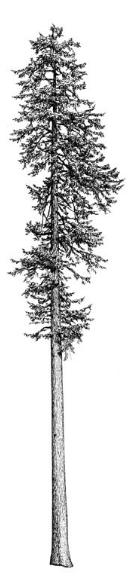
\includegraphics[width=.092\textwidth,angle=-1]{DougFir.png}};
							\draw   [thin,color=second](0,220) coordinate[label=above:$T$]--(90,70) coordinate[label=right:$P$]--(0,0) coordinate[label=below:$B$]--cycle;
        					\addplot[variable=\t, domain=30:90, samples=50,thin, color=third]({22*cos(t)}, {30*sin(t)});
        					\draw   (1,15)coordinate[label=right:\footnotesize$\ang{52}$];
        					\addplot[variable=\t, domain=127:210, samples=50,thin, color=third]({22*cos(t)+90}, {30*sin(t)+70});
        					\draw   (87,72)coordinate[label=left:\footnotesize$\ang{83}$];
        					\draw   (45,35)coordinate[label=below right:$115\text{ft}$];
					\end{axis}
				\end{tikzpicture}
			\end{center}
		\end{multicols}
		\vfill

		%======================================================
		\newpage
		%======================================================

		\item Imagine a triangle with sides $a=15$, $c=8$, and the angle $C=\ang{20}$, and length $b$, and angles $A$ and $B$ are unknown.
			\begin{enumerate}
				\item There are actually \emph{two} such triangles that exist. Draw pictures of both triangles.
				\vfill
				\item Write down the law of sines to solve for angle $A$ for each triangle, and compare the two equations.
				\vfill
				\item Solve for the angles and missing lengths in both triangles. Round your final answers for the angles and lengths to two digits behind the decimal place. \href{http://tiny.cc/ambiguous-triangles}{Check out this Desmos link} for a visual on these \say{ambiguous triangles}. \qrcode[height=1cm]{http://tiny.cc/ambiguous-triangles}
				\vfill
			\end{enumerate}
		\vfill
	\end{enumerate}
\end{myExit}
\exitlikert{the laws of sine and cosine}
\resetCounters
%============================================================
% MTH 112 Project - Polar Coordinates
% Updated 202504
%============================================================

\section{Polar Coordinates} \label{section-polar-coordinates}
In this section, we will learn a completely different way of organizing the coordinate plane: polar coordinates, where a polar point, $(r,\theta)$, has a radius $r$ from the origin and the angle from standard position, $\theta$. We will practice plotting points using polar coordinates, converting between polar coordinates and rectangular coordinates, transforming equations between polar and rectangular forms, and graphing polar equations.

\textbooks{\href{https://openstax.org/books/algebra-and-trigonometry-2e/pages/10-3-polar-coordinates}{10.3}}{\href{https://openstax.org/books/algebra-and-trigonometry-2e/pages/10-4-polar-coordinates-graphs}{10.4}}

\subsection*{Preparation Exercises} \label{preparation-exercises-section-polar-coordinates}

\begin{myPrep}
Answer the following without using a calculator. These questions are intended to check the prerequisite skills needed to complete the rest of the lab.
	\begin{multicols}{2}
		Thinking back to SOHCAHTOA, recall that for a triangle with legs $x$ and $y$ and hypotenuse $r$, as shown in Figure \ref{section-polar-coordinates-prep-triangle}, you know that $\cos(\theta)=\frac{x}{r}$, $\sin(\theta)=\frac{y}{r}$, and $\tan(\theta)=\frac{y}{x}$.
			\begin{center}\captionsetup{type=figure} \captionof{figure}{A right triangle}
				\begin{tikzpicture}[thin] \label{section-polar-coordinates-prep-triangle}
					\coordinate (O) at (0,0);
					\coordinate (A) at (3,0);
					\coordinate (B) at (0,2);
					\draw (O)--(A)--(B)--cycle;
					\footnotesize
					\tkzLabelSegment[below=2pt](O,A){$x$}
					\tkzLabelSegment[left=2pt](O,B){$y$}
					\tkzLabelSegment[above=2pt](A,B){$r$}
					\tkzMarkRightAngle[size=0.5](A,O,B)
					\tkzMarkAngle[size=0.8cm](B,A,O)
					\tkzLabelAngle[pos = 0.6](B,A,O){$\alpha$}
					\tkzMarkAngle[size=0.7cm](O,B,A)
					\tkzLabelAngle[pos = 0.5](O,B,A){$\beta$}
				\end{tikzpicture}
			\end{center}
		\columnbreak
			\begin{enumerate}[itemsep=1.5cm]
				\item Solve $\sin(\theta)=\frac{y}{r}$ for $y$.
				\item Solve $\cos(\theta)=\frac{x}{r}$ for $x$.
				\item What would the Pythagorean Theorem say about the triangle in Figure \ref{section-polar-coordinates-prep-triangle}?
			\end{enumerate}
	\end{multicols}
		% \begin{enumerate}\setcounter{enumi}{2}
		% \end{enumerate}
\end{myPrep}
\vfill

\begin{myPrep}
	What conditions would you need to put on $\theta$, $x$, and $y$ to make the solution to the equation $\tan(\theta)=\frac{y}{x}$ be $\theta=\tan^{-1}\left(\frac{y}{x}\right)$?
\end{myPrep}
\vfill
\vfill

\begin{myPrep}
	Which quadrant are the following angles in, when measured from the standard position.
		\begin{enumerate}
			\begin{multicols}{4}
				\item $\ang{400}$
				\item $\ang{-200}$
				\item $-\frac{7\pi}{6}$
				\item $\frac{17\pi}{3}$
			\end{multicols}
		\end{enumerate}
\end{myPrep}
\vfill

\begin{myPrep}
	Evaluate the expressions using your memorized values on the unit circle.
		\begin{enumerate}
			\begin{multicols}{4}
				\item $\sin(\ang{420})$
				\item $\cos(-\ang{210})$
				\item $\sin\left(-\frac{7\pi}{6}\right)$
				\item $\cos\left(\frac{17\pi}{3}\right)$
			\end{multicols}
		\end{enumerate}
\end{myPrep}
\vfill


%======================================================
\newpage
%======================================================

\subsection*{Practice Exercises} \label{practice-exercises-section-polar-coordinates}


\begin{myPractice}
	Practice plotting points written in polar form. For clarity, a small $_p$ will be written next to polar points to distinguish them from rectangular points, which will be written with a small $_r$ next to them. Label each point.
	\begin{multicols}{2}
		\begin{center}
			\captionsetup{type=figure} \captionof{figure}{A Polar Grid, with Standard Angles and Radii Shown}
			\begin{tikzpicture}
				\begin{axis}[
					xmin=-5,xmax=5,
					ymin=-5,ymax=5,
			       	xtick={1,2,3,4},
			       	ytick={1,2,3,4},
			       	clip=false,
					]
					\addplot[first,line width=1pt,opacity=0.2,samples=2] expression[domain=-5/sqrt(2):5/sqrt(2)]{x};
					\addplot[second,line width=1pt,opacity=0.2,samples=2] expression[domain=-2.5*sqrt(3):2.5*sqrt(3)]{1/sqrt(3)*x};
					\addplot[third,line width=1pt,opacity=0.2,samples=2] expression[domain=-2.5:2.5]{sqrt(3)*x};
					\addplot[first,line width=1pt,opacity=0.2,samples=2] expression[domain=-5/sqrt(2):5/sqrt(2)]{-x};
					\addplot[second,line width=1pt,opacity=0.2,samples=2] expression[domain=-2.5*sqrt(3):2.5*sqrt(3)]{-1/sqrt(3)*x};
					\addplot[third,line width=1pt,opacity=0.2,samples=2] expression[domain=-2.5:2.5]{-sqrt(3)*x};
					\draw[thin,opacity=0.2] (axis cs:0,0) circle [radius=1];
					\draw[thin,opacity=0.2] (axis cs:0,0) circle [radius=2];
					\draw[thin,opacity=0.2] (axis cs:0,0) circle [radius=3];
					\draw[thin,opacity=0.2] (axis cs:0,0) circle [radius=4];
					\draw[thin,opacity=0.2] (axis cs:0,0) circle [radius=5];
				\end{axis}
			\end{tikzpicture}
			\label{fig:section-polar-graph}
		\end{center}
			\columnbreak
			\begin{enumerate}[itemsep=0.3cm]
				\item $\left(4,\frac{\pi}{2}\right)_p$
				% \item $\left(2,\frac{4\pi}{3}\right)_p$
				\item $\left(3,-\frac{\pi}{4}\right)_p$
				\item $\left(-2,\frac{5\pi}{6}\right)_p$
				% \item $(1,\ang{120})_p$
				\item $(2.5,\ang{225})_p$
				\item $(3.5,-\ang{120})_p$
				\item $(-1.5,\ang{270})_p$
			\end{enumerate}
	\end{multicols}
\end{myPractice}

\begin{myPractice}
	Convert the polar points to rectangular form and the rectangular points to polar form. For clarity, a small $_p$ will be written next to polar points to distinguish them from rectangular points, which will be written with a small $_r$ next to them.
		\begin{enumerate}
			\item Find the rectangular coordinates of the polar points. Leave your answers in exact form rather than using your calculator to get a decimal value for the coordinates.
				\begin{enumerate}
					\begin{multicols}{2}
					\item $\left(4,\frac{\pi}{2}\right)_p$
					\vfill
					\item $\left(2,-\frac{4\pi}{3}\right)_p$
					\vfill
					% \item $(-1.5,\ang{270})_p$
					% \vfill
					\end{multicols}
				\end{enumerate}

	%======================================================
	\newpage
	%======================================================

		\item Find the polar coordinates of the rectangular points. 
			\begin{enumerate}
				\begin{multicols}{3}
				\item $(1,1)_r$. Leave your answers in exact form for both the radius and angle.
				\columnbreak
				% \item $\left(-3,\sqrt3\right)_r$. Leave your answers in exact form for both the radius and angle.
				\item $(2,3)_r$. Leave your radius in exact form, but use a calculator to find an approximation of the angle, accurate to three digits behind the decimal place.
				\columnbreak
				\item $(-2,-3)_r$. Leave your radius in exact form, but use a calculator to find an approximation of the angle, accurate to three digits behind the decimal place.
				\columnbreak
				\end{multicols}
			\end{enumerate}
		\end{enumerate}
\end{myPractice}
\vfill

\begin{myPractice}
	Convert equations between polar form and rectangular form. You can graph both the original equation and the polar form equation in Desmos to verify that you have converted correctly.
	\begin{enumerate}
		\item Convert the polar equations to rectangular form. You don't need to solve for a variable, necessarily. %https://www.desmos.com/calculator/abqlib6drm
			\begin{enumerate}
				\begin{multicols}{3}
					\item $r\cos(\theta)=5$ %solution $x=5$
					\item $r=3\sin(\theta)$ %solution $x^2+y^2=3y$
					\item $r=5$ %solution $x^2+y^2=25$
					% \item $r=\frac{3}{\cos(\theta)+2\sin(\theta)}$ %solution $x+2y=3$
				\end{multicols}
			\end{enumerate}
	\vfill
		\item Convert the rectangular equations to polar form. You don't need to solve for a variable, necessarily.
			\begin{enumerate}
				\begin{multicols}{3}
					\item $y=3$ %solution $r=\frac{3}{\sin(\theta)}$
					% \item $y=\frac{2}{x}$ %solution $r=\sqrt{\frac{2}{\sin(\theta)\cos(\theta)}}$
					\item $y=2x+1$ %solution $r=\frac{1}{\sin(\theta)-2\cos(\theta)}$
					\item $x^2+y^2=2x$ %solution $r=2\cos(\theta)$ or $r=0$
				\end{multicols}
			\end{enumerate}
	\vfill
	\end{enumerate}
\end{myPractice}

	%======================================================
	\newpage
	%======================================================

\begin{myPractice}
	Create a graph of the polar functions by filling in the tables and plotting points. Round the values of $r$ to the nearest tenth. Note that Desmos does have polar grid in the settings, and you can graph functions of the form $r=f(\theta)$, where the $\theta$ can be found in the \say{A B C} keyboard. A standardized Desmos template to create this table can be found in the link. \qrcode[height=1cm]{http://tiny.cc/PolarGraphTable}
	\begin{enumerate}
		\item
		\begin{multicols}{2}
			\begin{center}
				\renewcommand{\arraystretch}{1.5} 
				\begin{tabular}{|| c | P{3cm} ||}
					\hline
					$\theta$ & $r=2\sin(\theta)$ \\
					\hline
					$\ang{0}$ & \\ 
					\hline
					$\ang{30}$ & \\ 
					\hline
					$\ang{45}$ & \\ 
					\hline
					$\ang{60}$ & \\ 
					\hline
					$\ang{90}$ & \\ 
					\hline
					$\ang{120}$ & \\ 
					\hline
					$\ang{135}$ & \\ 
					\hline
					$\ang{150}$ & \\ 
					\hline
					$\ang{180}$ & \\
					\hline
				\end{tabular}
			\end{center}
		\columnbreak
			\begin{center}\captionsetup{type=figure} \captionof{figure}{A Polar Grid for the Graph of $r=2\sin(\theta)$}
				\begin{tikzpicture}
					\begin{axis}[
						height=8cm,
						width=8cm,
						xmin=-2.5,xmax=2.5,
						ymin=-2.5,ymax=2.5,
				       	xtick={1,1.5},
				       	ytick={1,1.5},
				       	clip=false,
						]
						\addplot[first,line width=1pt,opacity=0.2,samples=2] expression[domain=-2/sqrt(2):2/sqrt(2)]{x};
						\addplot[second,line width=1pt,opacity=0.2,samples=2] expression[domain=-sqrt(3):1*sqrt(3)]{1/sqrt(3)*x};
						\addplot[third,line width=1pt,opacity=0.2,samples=2] expression[domain=-1:1]{sqrt(3)*x};
						\addplot[first,line width=1pt,opacity=0.2,samples=2] expression[domain=-2/sqrt(2):2/sqrt(2)]{-x};
						\addplot[second,line width=1pt,opacity=0.2,samples=2] expression[domain=-sqrt(3):sqrt(3)]{-1/sqrt(3)*x};
						\addplot[third,line width=1pt,opacity=0.2,samples=2] expression[domain=-1:1]{-sqrt(3)*x};
						\draw[thin,opacity=0.2,dashed] (axis cs:0,0) circle [radius=0.5];
						\draw[thin,opacity=0.2] (axis cs:0,0) circle [radius=1];
						\draw[thin,opacity=0.2,dashed] (axis cs:0,0) circle [radius=1.5];
						\draw[thin,opacity=0.2] (axis cs:0,0) circle [radius=2];
						% \addplot[domain= 0:360] ({cos(x)},{sin(x)+1});
					\end{axis}
				\end{tikzpicture}\label{fig:section-polar-graph-of-2sin}
			\end{center}
		\end{multicols}
		\vfill

		\begin{multicols}{2}
			\item %Issue, fix this item numbering at top.
			\begin{center}
				\renewcommand{\arraystretch}{1.5} 
				\begin{tabular}{|| c | P{3cm} ||}
					\hline
					$\theta$ & $r=2\sin(3\theta)$ \\
					\hline
					$\ang{0}$ & \\ 
					\hline
					$\ang{30}$ & \\ 
					\hline
					$\ang{45}$ & \\ 
					\hline
					$\ang{60}$ & \\ 
					\hline
					$\ang{90}$ & \\ 
					\hline
					$\ang{120}$ & \\ 
					\hline
					$\ang{135}$ & \\ 
					\hline
					$\ang{150}$ & \\ 
					\hline
					$\ang{180}$ & \\
					\hline
				\end{tabular}
			\end{center}
		\columnbreak
			\begin{center}\captionsetup{type=figure} \captionof{figure}{A Polar Grid for a Graph of $r=2\sin(3\theta)$}
				\begin{tikzpicture}
					\begin{axis}[
						height=8cm,
						width=8cm,
						xmin=-2.5,xmax=2.5,
						ymin=-2.5,ymax=2.5,
				       	xtick={1,1.5},
				       	ytick={1,1.5},
				       	clip=false,
						]
						\addplot[first,line width=1pt,opacity=0.2,samples=2] expression[domain=-2/sqrt(2):2/sqrt(2)]{x};
						\addplot[second,line width=1pt,opacity=0.2,samples=2] expression[domain=-sqrt(3):1*sqrt(3)]{1/sqrt(3)*x};
						\addplot[third,line width=1pt,opacity=0.2,samples=2] expression[domain=-1:1]{sqrt(3)*x};
						\addplot[first,line width=1pt,opacity=0.2,samples=2] expression[domain=-2/sqrt(2):2/sqrt(2)]{-x};
						\addplot[second,line width=1pt,opacity=0.2,samples=2] expression[domain=-sqrt(3):sqrt(3)]{-1/sqrt(3)*x};
						\addplot[third,line width=1pt,opacity=0.2,samples=2] expression[domain=-1:1]{-sqrt(3)*x};
						\draw[thin,opacity=0.2,dashed] (axis cs:0,0) circle [radius=0.5];
						\draw[thin,opacity=0.2] (axis cs:0,0) circle [radius=1];
						\draw[thin,opacity=0.2,dashed] (axis cs:0,0) circle [radius=1.5];
						\draw[thin,opacity=0.2] (axis cs:0,0) circle [radius=2];
					\end{axis}
				\end{tikzpicture}\label{fig:section-polar-graph-of-2sin3}
			\end{center}
		\end{multicols}
		\vfill
		\item Visit \href{http://tiny.cc/polar-graphs}{this interactive Desmos graph} and change the values of $a$ and $b$. Find a particular graph that you like, write down it's equation, and discuss what you like about it with your neighbor. \qrcode[height=1cm]{http://tiny.cc/polar-graphs}
		\vfill
	\end{enumerate}
\end{myPractice}

%======================================================
\newpage
%======================================================

\subsection*{Definitions} \label{definitions-section-polar-coordinates}

\begin{myDefinition}[{Polar Functions}]~\\[0.5mm]
	A \textbf{polar function} is usually given in the form $r=f(\theta)$, where $\theta$ is the angle measured from the standard position along the positive $x$-axis, and $r$ is the radius measured from the origin.
\end{myDefinition}

\begin{myDefinition}[{Conversion formulas}]~\\[-0.5mm]
	\begin{itemize}
		\item To convert from rectangular form to polar form, use these two identities.
			\begin{enumerate}[itemsep=0.5cm]
				\item $r=\sqrt{x^2+y^2}$ or $r^2=x^2+y^2$
				\item $\tan(\theta)=\frac{y}{x}$
			\end{enumerate}
		\item To convert from polar form to rectangular form, use these two identities.
			\begin{enumerate}[itemsep=0.5cm]
				\item $x=r\cos(\theta)$
				\item $y=r\sin(\theta)$
			\end{enumerate}
	\end{itemize}
\end{myDefinition}

%======================================================
\newpage
%======================================================

\subsection*{Exit Exercises} \label{exit-exercises-section-polar-coordinates}

\begin{myExit}
	Which quadrant will the polar point $\left(-2,-\frac{7\pi}{6}\right)_p$ be in? Explain your answer.
\end{myExit}
\vfill

\begin{myExit}
	The graph of $r=2\cos(\theta)$ is a circle of radius 1 centered at $(1,0)_r$. Explain how $r$ \emph{is} a function of $\theta$ for this graph.
\end{myExit}
\vfill

\begin{myExit}
	A real-world machine used in fabrication uses polar coordinates. From a tripod setup, it has an extendable cord that comes out of a swiveling head on top of the unit that measures the distance to the end of the cord, and at what angle. This inputs a radius and angle into the computer. The machine then converts this polar point into a rectangular point and displays the resulting image on the screen. Fabrication can then begin. % https://www.desmos.com/calculator/lps0lwwoxq
		\begin{enumerate}
			\item The following polar coordinates were measured by the machine to form a new countertop. Convert them to rectangular coordinates and plot them in Desmos using the \say{polygon()} command. The units of measurement are in inches and degrees.
				\begin{enumerate}[itemsep=0.5cm]
					\item $(52,\ang{0})_p$
					\item  $(67.158,\ang{39.259})_p$
					\item $(42.5,\ang{90})_p$
					\item $(18.5,\ang{90})_p$
					\item  $(30.303,\ang{37.626})_p$
					\item $(24,\ang{0})_p$
				\end{enumerate}
			\vfill
			\item Find the total area of the countertop, in square feet. You can assume that the dimensions, as given, were intended to form right angles on the countertop.
			\vfill
		\end{enumerate}
\end{myExit}
\exitlikert{polar coordinates}
\resetCounters
%============================================================
% MTH 112 Project - Complex numbers
% Updated 202504
%============================================================

\section{Complex Numbers} \label{section-complex-numbers}
In this section, we will learn about complex numbers. We will learn how to plot complex numbers in the complex plane, convert complex numbers between polar, rectangular, and Euler forms, and how to arithmetic with complex numbers.

\textbooks{\href{https://openstax.org/books/algebra-and-trigonometry-2e/pages/10-5-polar-form-of-complex-numbers}{10.5}}{\href{https://openstax.org/books/algebra-and-trigonometry-2e/pages/2-4-complex-numbers}{2.4}}

\subsection*{Preparation Exercises} \label{preparation-exercises-section-complex-numbers}

Answer the following. These questions are intended to check the prerequisite skills needed to complete the rest of the lab.

\begin{myPrep}
	Convert the polar point $\left(4,\frac{7\pi}{6}\right)_p$ to rectangular form. Leave your components in exact form.
\end{myPrep}
\vfill

\begin{myPrep}
	Convert the rectangular point $(-5,2)_r$ to polar form. Use your calculator to find an angle in radians rounded to two digits behind the decimal place.
\end{myPrep}
\vfill

\begin{myPrep}
	\begin{multicols}{2}
		For the right triangle shown in Figure \ref{section-complex-numbers-triangle-solving}, find the missing length of $r$ and the missing angle $\theta$ using SOHCAHTOA. You can use a calculator to help get an approximation, accurate to 4 digits behind the decimal place.
			\columnbreak
			\begin{center}\captionsetup{type=figure} \captionof{figure}{A right triangle}
				\begin{tikzpicture}[thin] \label{section-complex-numbers-triangle-solving}
					\coordinate (O) at (0,0);
					\coordinate (A) at (5,0);
					\coordinate (B) at (5,2);
					\draw (O)--(A)--(B)--cycle;
					\footnotesize
					\tkzLabelSegment[below=2pt](O,A){$5\text{cm}$}
					\tkzLabelSegment[above=2pt](O,B){$r$}
					\tkzLabelSegment[right=2pt](A,B){$2\text{cm}$}
					\tkzMarkRightAngle[size=0.5](B,A,O)
					\tkzMarkAngle[size=1.3cm](A,O,B)
					\tkzLabelAngle[pos = 1](A,O,B){$\theta$}
				\end{tikzpicture}
			\end{center}
	\end{multicols}
\end{myPrep}
\vfill
\vfill

%======================================================
\newpage
%======================================================

\subsection*{Practice Exercises} \label{practice-exercises-section-complex-numbers}

\begin{myPractice}
		\begin{multicols}{2}
			Plot the complex numbers onto Figure \ref{section-complex-numbers-practice-plotting}.
				\begin{enumerate}[itemsep=.5cm]
					\item $2+3i$
					\item $-1+2i$
					\item $-3i$
					\item $3-i$
				\end{enumerate}
				\columnbreak
				\begin{center}\captionsetup{type=figure} \captionof{figure}{A complex plane}
					\begin{tikzpicture}[thin] \label{section-complex-numbers-practice-plotting}
 						\begin{axis}[
 							height=6cm,
 							width=6cm,
 							framed,
 							ylabel={$y_i$},
 							xmin=-4,xmax=4,
 							ymin=-4,ymax=4,
						    xtick={-3,-2,...,3},
						    ytick={-3,-2,...,3},
						    grid=both,
 							]
 						\end{axis}
					\end{tikzpicture}
				\end{center}
		\end{multicols}
\end{myPractice}

\begin{myPractice}
		Find the absolute value and argument of the complex numbers.
			\begin{enumerate}
				\begin{multicols}{2}
					\item $2+3i$
					\item $-1+2i$
				\end{multicols}
			\end{enumerate}
		\vfill
\end{myPractice}

\begin{myPractice}
	\begin{enumerate}
		\item Convert the standard form complex number $5-12i$ into polar form. Use radians and round your argument to two digits behind the decimal place.
		\vfill
		\item Convert the polar form complex number $7\left(\cos\left(\frac{5\pi}{6}\right)+i\sin\left(\frac{5\pi}{6}\right)\right)$ into standard form. Keep your values exact using your memorized values on the unit circle.
		\vfill
	\end{enumerate}
\end{myPractice}

%======================================================
\newpage
%======================================================

\begin{myPractice}
	Simplify the expressions completely.
	\begin{enumerate}[itemsep=3cm]
		\begin{multicols}{2}
			\item $(2i)^4$
			\item $(2i+3)-(4i-1)$
			\columnbreak
			\item $(2i+3)\cdot(4i-1)$
		\end{multicols}
	\end{enumerate}
\end{myPractice}
\vfill

\begin{myPractice}
	\begin{enumerate}
		\item Convert the standard form complex number $5-12i$ into Euler's form. Use radians and round your argument to two digits behind the decimal place.
		\vfill
		\item Convert the Euler's form complex number $7e^{\frac{4\pi i}{3}}$ into standard form. Keep your values exact using your memorized values on the unit circle.
		\vfill
	\end{enumerate}
\end{myPractice}

%======================================================
\newpage
%======================================================

\subsection*{Definitions} \label{definitions-section-complex-numbers}

\begin{myDefinition}[The Imaginary unit $i$]
The \textbf{imaginary unit $i$} is defined to be $i=\sqrt{-1}$. Since there is no real number that is multiplied by itself to create a negative number, $i$ must not be a real number. It fits into a new category of numbers called imaginary numbers which are any multiples of $i$. It's called a \say{unit} because its absolute value is $1$.
\newline For example, $4i$, $-2i$, and $\sqrt{-9}$ are all imaginary numbers.
\end{myDefinition}

\begin{myDefinition}[{Standard form of a Complex Number}]~\\[0.5mm]
A \textbf{complex number} is any real number plus any imaginary number. Any complex number can be written in standard form (also called rectangular form), which is the form $a+bi$, where both $a$ and $b$ are real numbers. 
\newline For example, $3+0i$, $0-2i$, and $1-\sqrt{5}i$ are all complex numbers.
\end{myDefinition}

\begin{myDefinition}[{The Complex plane}]~\\[0.5mm]
The \textbf{complex plane} is the two dimensional axes system to plot complex numbers. The horizontal axis, often just labeled $x$, measures the real part of a complex number. The vertical axis, often labeled $y_i$, measures the imaginary part of a complex number. 
\newline For example, the number $-3+4i$ would be plotted $3$ units to the left and $4$ units up from the origin at the same place that $(-3,4)$ would have been plotted in the regular two-dimensional real axes.
\end{myDefinition}

\begin{myDefinition}[{Absolute Value of a Complex number}]~\\[0.5mm]
The \textbf{absolute value of the complex number} is the distance from the origin to the number in the complex plane. The absolute value is written as usual, $\abs{z}$. To find the absolute value of $z=a+bi$, use the Pythagorean Theorem: $\abs{z}=\sqrt{a^2+b^2}$. 
\newline \emph{Note}: the $i$ is \emph{dropped} during this calculation! 
\newline \emph{Note}: the absolute value of a complex number is sometimes also called the magnitude or modulus.
\newline For Example, to find the absolute value of $z=-3+4i$, we would write that $\abs{z}=\sqrt{(-3)^2+4^2}=5$. 
\end{myDefinition}

\begin{multicols}{2}
	\begin{myDefinition}[{Argument of a Complex number}]~\\[0.5mm]
	The \textbf{argument of the complex number}, $z=a+bi$, is an angle, $\theta$ measured from the standard position to the number in the complex plane. To find this angle, $\theta$, use the formula $\tan(\theta)=\frac{b}{a}$ and solve for $\theta$ that is in the correct quadrant. 
	\newline \emph{Note}: the $i$ is \emph{dropped} during this calculation! 
	\newline For example, to find the argument of $z=-3+4i$, we would first note that $z$ is in the second quadrant, and we would write $\tan(\theta)=\frac{4}{-3}$. Next, we would take the inverse-tangent on both sides, \emph{however}, inverse-tangent does not give us angles in quadrant II, so we know that to find the correct argument of $z$ we should add $\pi$. So the argument of $z$ is $\theta=\tan^{-1}\left(\frac{4}{-3}\right)+\pi\approx2.21$, as shown in Figure \ref{section-complex-numbers-abs-val-and-argument}.
	\end{myDefinition}

	\begin{center}\captionsetup{type=figure} \captionof{figure}{A graph of $z=-3+4i$ showing the absolute value and argument of $z$}
		\begin{tikzpicture}[thin] \label{section-complex-numbers-abs-val-and-argument}
 			\begin{axis}[
 				framed,
 				ylabel={$y_i$},
 				xmin=-4,xmax=2,
 				ymin=-1,ymax=5,
			    xtick={-3,-2,-1,1},
			    ytick={1,2,3,4},
			    grid=both,
 				]
 				\draw 	(-3,4) node[above,color=first] {$-3+4i$};
 				\draw 	(1,1.3) node[color=third] {$\theta\approx2.21$};
				\addplot[only marks, mark=*,color=first] coordinates{(-3,4)(0,0)};
				\addplot[dashed,color=second,thin] coordinates{(-3,4)(0,0)};
				\addplot[domain= 0:126.87,third] ({cos(x)},{sin(x)});
				\draw 	(-1.5,2) node[above,color=second,rotate=-atan(4/3)] {$\abs{z}=5$};
 			\end{axis}
		\end{tikzpicture}
	\end{center}
\end{multicols}

\begin{myDefinition}[{Polar form of a Complex number}]~\\[0.5mm]
A complex number can be written in \textbf{polar form}, which is the form $r\left(\cos(\theta)+i\sin(\theta)\right)$, where $r=\abs{z}$ and and $\theta$ is the argument of the complex number. 
\newline For example, $z=-3+4i$ can be written as $z\approx5\left(\cos(2.21)+i\sin(2.21)\right)$. 
\newline \emph{Note}: We used the $\approx$ symbol here because the $2.21$ was an approximate value. 
\newline \emph{Note}: $\cos(\theta)+i\sin(\theta)$ is sometimes called $\text{cis}(\theta)$.
\end{myDefinition}

\begin{myDefinition}[{Euler's form of a Complex number}]~\\[0.5mm]
\textbf{Euler's form} of a complex number, $z$, is $z=re^{i\theta}$, where $r=\abs{z}$ and $\theta$ is the argument of $z$. 
\newline For example, $z=-3+4i$ can be written as $z\approx5e^{i\cdot2.21}$. 
\newline \emph{Note}: We used the $\approx$ symbol here because the $2.21$ was an approximate value.
\end{myDefinition}

%======================================================
\newpage
%======================================================

\subsection*{Exit Exercises} \label{exit-exercises-section-complex-numbers}

\begin{myExit}
	Describe the difference between the point $(5,8)$ in the two-dimensional real coordinate plane and the complex number $5+8i$ in the complex plane.
\end{myExit}

\begin{myExit}
	\begin{enumerate}
		\begin{multicols}{2}
			\item Plot the complex number $-6-4i$ onto Figure \ref{section-complex-numbers-exit-plotting}.
			\item Find the absolute value of the complex number $-6-4i$. Simplify the radical completely and leave your answer in exact form. Illustrate this value on Figure \ref{section-complex-numbers-exit-plotting}.
			\vfill
			\item Find the argument of the complex number \newline$-6-4i$. Use a calculator to round your answer to three digits behind the decimal place. Illustrate this value on Figure \ref{section-complex-numbers-exit-plotting}.
			\vfill
			\columnbreak
			\begin{center}\captionsetup{type=figure} \captionof{figure}{A complex plane to plot complex numbers}
				\begin{tikzpicture}[thin] \label{section-complex-numbers-exit-plotting}
 					\begin{axis}[
 						framed,
 						ylabel={$y_i$},
 						xmin=-7,xmax=7,
 						ymin=-7,ymax=7,
					    xtick={-6,-5,...,6},
					    ytick={-6,-5,...,6},
					    grid=both,
 						]
 					\end{axis}
				\end{tikzpicture}
			\end{center}
		\end{multicols}
	\end{enumerate}
	\begin{enumerate}\setcounter{enumi}{3}
		\vfill
		\item Write the complex number $-6-4i$ into polar form. 
		\vfill
		\item Write the complex number $-6-4i$ into Euler's form. 
		\vfill
	\end{enumerate}
\end{myExit}
\exitlikert{complex numbers}
\resetCounters
%============================================================
% MTH 112 Project - Vectors
% Updated 202504
%============================================================

\section{Vectors} \label{section-vectors}
In this section, we will learn about vectors, which are essentially a line segment with a specific length and that points in a particular direction. We will view vectors geometrically, find the magnitude and direction of vectors, find the component form of a vector, and do arithmetic with vectors. Then we will find the dot product of two vectors and work through some applications of vectors.

\textbook{\href{https://openstax.org/books/algebra-and-trigonometry-2e/pages/10-8-vectors}{10.8}}

\subsection*{Preparation Exercises} \label{preparation-exercises-section-vectors}

Answer the following without using a calculator. These questions are intended to check the prerequisite skills needed to complete the rest of the lab.

\begin{myPrep}
	\begin{multicols}{2}
		For the right triangle shown in Figure \ref{section-vectors-triangle-solving}, find the missing lengths of $x$ and $y$ using SOHCAHTOA. You can use a calculator to help get an approximation, accurate to 4 digits behind the decimal place.
		\columnbreak
		\begin{center}\captionsetup{type=figure} \captionof{figure}{A right triangle}
			\begin{tikzpicture}[thin] \label{section-vectors-triangle-solving}
				\coordinate (O) at (0,0);
				\coordinate (A) at (3,0);
				\coordinate (B) at (3,2);
				\draw (O)--(A)--(B)--cycle;
				\footnotesize
				\tkzLabelSegment[below=2pt](O,A){$x$}
				\tkzLabelSegment[above=2pt,rotate=atan(2/3)](O,B){$10\text{cm}$}
				\tkzLabelSegment[right=2pt](A,B){$y$}
				\tkzMarkRightAngle[size=0.5](B,A,O)
				\tkzMarkAngle[size=0.7cm](A,O,B)
				\tkzLabelAngle[pos = 1.1](A,O,B){$\ang{32}$}
			\end{tikzpicture}
		\end{center}
	\end{multicols}
\end{myPrep}
\vfill

\begin{myPrep}
	\begin{enumerate}
		\item Convert the polar point $\left(8,\frac{2\pi}{3}\right)_p$ to rectangular coordinates. Leave your coordinates in exact form using memorized values from the unit circle.
		\vfill
		\item Write the complex number $3+4i$ in Euler's form, $re^{i\theta}$. Write your angle in radians and round it to 2 digits behind the decimal place.
		\vfill
		\item Convert the rectangular point $(3,4)_r$ to polar form. Write your angle in radians and round it to 2 digits behind the decimal place.
		\vfill
	\end{enumerate}
\end{myPrep}
\vfill

%======================================================
\newpage
%======================================================

\subsection*{Practice Exercises} \label{practice-exercises-section-vectors}

\begin{myPractice}
	\begin{multicols}{2}
		\begin{enumerate}
			\item Draw a vector, $\vectr{g}$, onto Figure \ref{section-vectors-practice-plotting} that goes from point $(-3,2)$ to point $(2,-1)$.
			\vfill
			\item Draw another copy of $\vectr{g}$ onto Figure \ref{section-vectors-practice-plotting}, this one starting from the origin.
			\vfill
			\item Write $\vectr{g}$ in component form using the angled-bracket notation, $\vect{\ph{m}}{\ph{m}}$.
			\vfill
		\end{enumerate}
		\begin{center}\captionsetup{type=figure} \captionof{figure}{A grid to plot a vector}
			\begin{tikzpicture}[thin] \label{section-vectors-practice-plotting}
 				\begin{axis}[
 					framed,
					xmin=-5,xmax=5,
 					ymin=-5,ymax=5,
				    xtick={-4,-3,...,4},
				    ytick={-4,-3,...,4},
				    grid=both,
 					]
 				\end{axis}
			\end{tikzpicture}
		\end{center}
	\end{multicols}
	\begin{enumerate}\setcounter{enumi}{3}
		\item Write $\vectr{g}$ in component form using the $a\unitv{i}+b\unitv{j}$ notation.
		\vspace{1cm}
		\item Find $\norm{\vectr{g}}$, the magnitude of $\vectr{g}$.
		\vspace{1cm}
		\item Find $\theta$, the direction of $\vectr{g}$, measured in degrees from the standard position. Round your answer to two digits behind the decimal place.
		\vspace{2cm}
	\end{enumerate}
\end{myPractice}

\begin{myPractice}
	Perform the vector arithmetic.
	\begin{enumerate}
		\begin{multicols}{2}
			\item $\vect{-2}{6}+\vect{4}{-3}$
			\vspace{0.9cm}
			\item $\left(-5\unitv{i}-2\unitv{j}\right)-\left(6\unitv{i}-4\unitv{j}\right)$
			\vspace{0.9cm}
			\item $3\vect{4}{-7}$
			\item $5\left(2\unitv{i}-1\unitv{j}\right)-4\left(-4\unitv{i}+3\unitv{j}\right)$
			\vspace{0.9cm}
			\item $\left(-3\unitv{i}+5\unitv{j}\right)\cdot\left(4\unitv{i}+2\unitv{j}\right)$
			\vspace{0.9cm}
			\item $\vect{-6}{3}\cdot\vect{2}{9}$
		\end{multicols}
	\end{enumerate}
\end{myPractice}
\vfill
\newpage
\begin{myPractice}
	Are the vectors in the same direction, perpendicular, or skew? Consider using the dot product to show that vectors are perpendicular since two vectors are perpendicular if and only if their dot product is $0$.
	\begin{multicols}{2}
		\begin{enumerate}[itemsep=1cm]
			\item $\vect{6}{-6}$ and $\vect{1}{-1}$?
			\item $\vect{5}{-6}$ and $\vect{-5}{6}$?
			\item $\vect{-6}{2}$ and $\vect{3}{9}$?
			\item $\vect{6}{-1}$ and $\vect{1}{-4}$?
		\end{enumerate}
	\end{multicols}
\end{myPractice}
\vspace{1cm}
\begin{myPractice}
	% \begin{enumerate}
	% 	\item 
		Find a unit vector, $\unitv{u}_1$, in direction of $\vectr{v}=3\unitv{i}+4\unitv{j}$.
	% 	\vfill
	% 	\item Find a unit vector, $\unitv{u}_2$, in direction of $\vectr{w}=\vect{-2}{6}$. Simplify and rationalize the denominator of your answer.
		\vfill
	% \end{enumerate}
\end{myPractice}

\begin{myPractice}
	If a vector, $\vectr{p}$, has a magnitude $\norm{\vectr{p}}=16$ and a direction angle of $\theta=\ang{260}$, use a calculator to find the approximate components of $\vectr{p}$, rounded to two digits behind the decimal place.
\end{myPractice}
\vfill

%======================================================
\newpage
%======================================================

\begin{myPractice}
	Find the angle between the two vectors $\vectr{m}=\vect{-1}{4}$ and $\vectr{n}=\vect{2}{1}$ using the formula $\vectr{m}\cdot\vectr{n}=\norm{\vectr{m}}\norm{\vectr{n}}\cos(\theta)$
	\vfill
\end{myPractice}

\begin{myPractice}
	Jamal and Jenna did a dive in the Columbia River while taking an advanced SCUBA class. It was cold, dark, and muddy. They dove to the deepest part of the river, enjoyed a fast-paced drift dive, and started toward shore well below the surface to avoid boat traffic. They swam at a pace of $2\frac{ft}{s}$ (relative to the water around them) toward shore at a bearing of $\ang{310}$ on his compass. The river was pushing them at a pace of $8\frac{ft}{s}$ at a bearing of $\ang{230}$. They felt like they were spinning in circles, but managed to get to shore safely.
	\begin{enumerate}
		\item Find the component form of $\vectr{s}$, the vector that represents their swimming velocity, ignoring that the water around them is moving, assuming that the positive $x$-axis aligns with East.
		\vfill
		\item Find the component form of $\vectr{r}$, the vector that represents the river's velocity.
		\vfill
		\item Find the sum $\vectr{s}+\vectr{r}$, and interpret its meaning in terms of the divers and the river.
		\vfill
	\end{enumerate}
\end{myPractice}
%======================================================
\newpage
%======================================================

\subsection*{Definitions} \label{definitions-section-vectors}

\begin{multicols}{2}
	\begin{myDefinition}[{Vector}]~\\[0.5mm]
	A \textbf{vector} is a quantity drawn as a line segment with an arrowhead at one end. It has an initial point, where it begins, and a terminal point, where it ends. It is a line segment with a direction. Vectors are placement-independent in that two vectors that are the same length and parallel are considered the same vector, as shown in Figure \ref{section-vectors-definition-vector}. Vector notation is usually either \say{the vector $\overrightharp{\textbf{v}}$} or \say{the vector $\vectr{v}$}
	\end{myDefinition}

	\columnbreak

	\begin{center}\captionsetup{type=figure} \captionof{figure}{Two copies of the vector $\vectr{v}$}
		\begin{tikzpicture}[thin] \label{section-vectors-definition-vector}
	 		\begin{axis}[
	 			framed,
	 			height=5cm,
	 			width=5cm,
	 			xmin=-2,xmax=3,
	 			ymin=-2,ymax=3,
			    xtick=\empty,
			    ytick=\empty,
			    grid=both,
	 			]
				\addplot[ultra thick,->,color=first] coordinates{(0,0)(1,2)};
				\node[color=first] at (.8, 1) {$\vectr{v}$};
				\addplot[ultra thick,->,color=first] coordinates{(1,-1.5)(2,.5)};
				\node[color=first] at (1.8, -.5) {$\vectr{v}$};
	 		\end{axis}
		\end{tikzpicture}
	\end{center}
\end{multicols}

\begin{multicols}{2}
	\begin{myDefinition}[{The vectors $\unitv{i}$ and $\unitv{j}$}]~\\[0.5mm]
	The \textbf{vector $\unitv{i}$} (read \say{i hat}) is defined to be a vector of length $1$ pointed to the right (parallel to the positive $x$-axis) \textbf{and $\unitv{j}$} (read \say{j hat}) is defined to be a vector of length $1$ pointed up (parallel to the positive $y$-axis), as shown in Figure \ref{section-vectors-definition-ij}. We always use a \say{hat} on unit vectors instead of an arrow.
	\end{myDefinition}

	\columnbreak

	\begin{center}\captionsetup{type=figure} \captionof{figure}{The vectors $\unitv{i}$ and $\unitv{j}$}
		\begin{tikzpicture}[thin] \label{section-vectors-definition-ij}
	 		\begin{axis}[
	 			framed,
	 			height=5cm,
	 			width=5cm,
	 			xmin=-1,xmax=2,
	 			ymin=-1,ymax=2,
			    xtick={1},
			    ytick={1},
			    grid=both,
	 			]
				\addplot[ultra thick,->,color=first] coordinates{(0,0)(1,0)};
				\node[color=first] at (.5, -.25) {$\unitv{i}$};
				\addplot[ultra thick,->,color=second] coordinates{(0,0)(0,1)};
				\node[color=second] at (-.25, .5) {$\unitv{j}$};
	 		\end{axis}
		\end{tikzpicture}
	\end{center}
\end{multicols}

\begin{multicols}{2}
	\begin{myDefinition}[{The components of a vector}]~\\[0.5mm]
	If you take a vector, $\vectr{v}$, and create a right triangle where the vector is the hypotenuse and the legs of the triangle are horizontal and vertical, then \textbf{the components vector} $\vectr{v}$ are the vertical and horizontal vectors that add together to form $\vectr{v}$, as shown in Figure \ref{section-vectors-definition-components}. Since the components are horizontal and vertical, we measure them with $\unitv{i}$'s and $\unitv{j}$'s.
	\end{myDefinition}

	\begin{myDefinition}[{The magnitude of a vector}]~\\[0.5mm]
	The \textbf{magnitude of a vector}, $\vectr{v}=\vect{v_1}{v_2}$, is the length of the vector and is written $\norm{\vectr{v}}$ We use the Pythagorean theorem on the components of the vector to find a formula for the magnitude:
	\[\norm{\vectr{v}}=\sqrt{v_1^2+v_2^2}\]
	\end{myDefinition}

	\columnbreak

	\begin{center}\captionsetup{type=figure} \captionof{figure}{The vector $\vectr{v}=4\unitv{i}+3\unitv{j}$, its components, magnitude, and direction shown}
		\begin{tikzpicture}[thin] \label{section-vectors-definition-components}
	 		\begin{axis}[
	 			framed,
	 			xmin=-1,xmax=5,
	 			ymin=-1,ymax=5,
			    xtick={1,2,3,4},
			    ytick={1,2,3,4},
			    grid=both,
	 			]
	 			\addplot[ultra thick,->,color=third] coordinates{(0,0)(4,3)};
				\node[color=third] at (3.8, 3.3) {$\vectr{v}$};
				\node[color=third,rotate=atan(3/4)] at (2, 2) {$\norm{\vectr{v}}=5$};
				\addplot[very thick,->,color=first] coordinates{(0,0)(1,0)};
				\addplot[very thick,->,color=first] coordinates{(1,0)(2,0)};
				\addplot[very thick,->,color=first] coordinates{(2,0)(3,0)};
				\addplot[very thick,->,color=first] coordinates{(3,0)(4,0)};
				\node[color=first] at (0.5, -.25) {$\unitv{i}$};
				\node[color=first] at (1.5, -.25) {$\unitv{i}$};
				\node[color=first] at (2.5, -.25) {$\unitv{i}$};
				\node[color=first] at (3.5, -.25) {$\unitv{i}$};
				\addplot[very thick,->,color=second] coordinates{(4,0)(4,1)};
				\addplot[very thick,->,color=second] coordinates{(4,1)(4,2)};
				\addplot[very thick,->,color=second] coordinates{(4,2)(4,3)};
				\node[color=second] at (4.25, 0.5) {$\unitv{j}$};
				\node[color=second] at (4.25, 1.5) {$\unitv{j}$};
				\node[color=second] at (4.25, 2.5) {$\unitv{j}$};
				\addplot[thin,domain= 0:atan(3/4),color=fourth] ({cos(x)},{sin(x)});
				\node[color=fourth] at (1.2,0.4) {$\theta$};
	 		\end{axis}
		\end{tikzpicture}
	\end{center}
\end{multicols}

%======================================================
\newpage
%======================================================

\begin{myDefinition}[{The direction of a vector}]~\\[0.5mm]
	The \textbf{direction of a vector} is defined by an angle, $\theta$, relative to the standard position (unless otherwise specified), positioned at the initial point of the vector.
\end{myDefinition}

\begin{myDefinition}[{Graphically adding two vectors}]~\\[0.5mm]
	\begin{minipage}{0.9\textwidth}
        To graphically add two vectors, $\vectr{v}+\vectr{w}$, put the tail of vector $\vectr{w}$ at the head of $\vectr{v}$. The sum, $\vectr{v}+\vectr{w}$, is the vector from the tail of $\vectr{v}$ to the head of $\vectr{w}$. Check out \href{http://tiny.cc/vector-addition}{this Desmos link} for a visual on graphical vector addition.
    \end{minipage}
	\begin{minipage}{2cm}
        \qrcode[height=1cm]{http://tiny.cc/vector-addition}
    \end{minipage}
\end{myDefinition}

\begin{myDefinition}[{Graphically subtracting two vectors}]~\\[0.5mm]
	\begin{minipage}{0.9\textwidth}
    	To graphically subtract two vectors, $\vectr{v}-\vectr{w}$, first draw the opposite vector of $\vectr{w}$, which would be $-\vectr{w}$ drawn with the same length as $\vectr{w}$ but exactly $\ang{180}$ from $\vectr{w}$. Then put the tail of vector $-\vectr{w}$ at the head of $\vectr{v}$. The difference, $\vectr{v}-\vectr{w}$, is the vector from the tail of $\vectr{v}$ to the head of $-\vectr{w}$. This process really creates $\vectr{v}+(-\vectr{w})$. Check out \href{http://tiny.cc/vector-subtraction}{this Desmos link} for a visual on graphical vector subtraction.
	\end{minipage}
	\begin{minipage}{2cm}
    	\qrcode[height=1cm]{http://tiny.cc/vector-subtraction}
	\end{minipage}
\end{myDefinition}

\begin{myDefinition}[{A unit vector}]~\\[0.5mm]
	A \textbf{unit vector} is a vector of magnitude $1$. There is a formula that takes any vector, $\vectr{v}$, and will find a unit vector, $\unitv{u}$, in the same direction as $\vectr{v}$:
\[\unitv{u}=\frac{\vectr{v}}{\norm{\vectr{v}}}\]
\end{myDefinition}

\begin{myDefinition}[{The dot product of two vectors}]~\\[0.5mm]
	The \textbf{dot product} of two vectors, $\vectr{v}=\vect{v_1}{v_2}$ and $\vectr{w}=\vect{w_1}{w_2}$, is the sum of the product of the corresponding components of the vectors: 
		\[\vectr{v}\cdot\vectr{w}=v_1w_1+v_2w_2\] 
	This happens to tell you something about how far apart the vectors are, angle-wise. There is a relationship between the dot product and the angle, $\theta$, between the vectors: 
		\[\vectr{v}\cdot\vectr{w}=\norm{\vectr{v}}\norm{\vectr{w}}\cos(\theta)\]
	Note that this implies that two vectors are perpendicular if and only if their dot product is $0$ since cosine is only $0$ when the angle is a right angle. To be more specific, cosine is only $0$ when the angle is an odd multiple of $\frac{\pi}{2}$.
\end{myDefinition}

%======================================================
\newpage
%======================================================

\subsection*{Exit Exercises} \label{exit-exercises-section-vectors}

\begin{myExit}
	Answer the following where $\vectr{t}=\vect{-1}{-3}$ and $\vectr{s}=\vect{3}{2}$.
	\begin{enumerate}[itemsep=5mm]
		\begin{multicols}{2}\raggedcolumns
		\item Draw $\vectr{t}$ and $\vectr{s}$ onto Figure \ref{section-vectors-exit}.
		\item Draw $\vectr{t}+\vectr{s}$ onto Figure \ref{section-vectors-exit}.
		\item Evaluate $3\vectr{t}-2\vectr{s}$.
		\vspace{2cm}
		\item Evaluate $\vectr{t}\cdot\vectr{s}$.
		\columnbreak
		\begin{center}\captionsetup{type=figure} \captionof{figure}{A grid to draw $\vectr{t}$ and $\vectr{s}$}\label{section-vectors-exit}
			\begin{tikzpicture}[thin]
		 		\begin{axis}[
		 			framed,
		 			xmin=-5,xmax=5,
		 			ymin=-5,ymax=5,
				    xtick={-4,-3,...,4},
				    ytick={-4,-3,...,4},
				    grid=both,
		 			]
	 				% \addplot[ultra thick,->,color=first] coordinates{(0,0)(3,2)}; %solutions
	 				% \addplot[ultra thick,->,color=second] coordinates{(0,0)(-1,-3)}; %solutions
	 				% \addplot[ultra thick,->,color=second] coordinates{(3,2)(2,-1)}; %solutions
	 				% \addplot[ultra thick,->,color=third] coordinates{(0,0)(2,-1)}; %solutions
		 		\end{axis}
			\end{tikzpicture}
		\end{center}
	\end{multicols}
		\item Evaluate $\norm{\vectr{t}}$.
		\vfill
		\item What is the direction of $\vectr{t}$? Use degrees and round your answer to two digits behind the decimal place.
		\vfill
		\item Find the angle between $\vectr{t}$ and $\vectr{s}$ using the dot product.
		\vfill
	\end{enumerate}
\end{myExit}
\exitlikert{vectors}
% \resetCounters
% \include{112-chapter-supplement-applications-of-trig}

\end{document}

% Optional Topics
% \resetCounters
% \include{112-section-parametric-equations}